%%!TEX root = ./marylie.tex
%%--.----1----.----2----.----3----.----4----.----5----.----6----.----7----.-!

\chapter{Catalog of Advanced Commands}
     Because \Mary works with explicit representations of transfer maps, there are almost unlimited possibilities for commands to manipulate and analyze these maps.  Listed below are the advanced map analysis and manipulation commands, with their type-code mnemonics, that are currently available in \Mary 3.0.  Also listed are the subsections that describe them in detail.  It is expected that additional advanced commands will be added in the future.\index{commands} \index{advanced commands}

\begin{center}
\begin{tabular}{lll}
\multicolumn{1}{c}{\underline {Type Code}} &
\multicolumn{1}{c}{\underline{Command}}   &
\multicolumn{1}{c}{\underline{Subsection}} \\
\hspace{1.5em}cod     &   Compute off-momentum closed orbit data.  & \hspace{2em}8.1\\
\vspace{-3mm}& &\\
\hspace{1.5em}tasm    &           Twiss analyze static map.      &  \hspace{2em}8.2\\
\vspace{-3mm}& &\\
\hspace{1.5em}tadm    &           Twiss analyze dynamic map.     &  \hspace{2em}8.3\\
\vspace{-3mm}& &\\
\hspace{1.5em}rasm    &           Resonance analyze static map.  &  \hspace{2em}8.4\\
\vspace{-3mm}& &\\
\hspace{1.5em}radm    &           Resonance analyze dynamic map. &  \hspace{2em}8.5\\
\vspace{-3mm}& &\\
\hspace{1.5em}tbas    &           Translate basis.               &  \hspace{2em}8.6\\
\vspace{-3mm}& &\\
\hspace{1.5em}exp     &           Compute exponential.           &  \hspace{2em}8.7\\
\vspace{-3mm}& &\\
\hspace{1.5em}snor    &           Static normal form analysis.   &  \hspace{2em}8.8\\
\vspace{-3mm}& &\\
\hspace{1.5em}dnor    &           Dynamic normal form analysis.  &  \hspace{2em}8.9\\
\vspace{-3mm}& &\\
\hspace{1.5em}sia     &           Static invariant analysis.     &  \hspace{2em}8.10\\
\vspace{-3mm}& &\\
\hspace{1.5em}dia     &           Dynamic invariant analysis.    &  \hspace{2em}8.11\\
\vspace{-3mm}& &\\
\hspace{1.5em}psnf    &    Compute power of static normal form.&  \hspace{2em}8.12\\
\vspace{-3mm}& &\\
\hspace{1.5em}pdnf    &    Compute power of dynamic normal form.&  \hspace{2em}8.13\\
\vspace{-3mm}& &\\
\hspace{1.5em}gbuf    &           Get buffer contents.           &
\hspace{2em}8.14\\
\vspace{-3mm}& &\\
\hspace{1.5em}fasm    &           Fourier analyze static map.    &  \hspace{2em}8.15\\
\vspace{-3mm}& &\\
\hspace{1.5em}fadm    &           Fourier analyze dynamic map.   &  \hspace{2em}8.16
\end{tabular}

\begin{tabular}{lll}
\multicolumn{1}{c}{\underline{Type Code}} &
\multicolumn{1}{c}{\underline{Command}}   &
\multicolumn{1}{c}{\underline{Subsection}} \\
\hspace{1.5em}amap    &     Apply map to a function or moments.  &   \hspace{2em}8.17\\
\vspace{-3mm}& &\\
\hspace{1.5em}smul    &      Multiply a polynomial by a scalar.    & \hspace{2em}8.18\\
\vspace{-3mm}& &\\
\hspace{1.5em}padd    &           Add two polynomials.       &   \hspace{2em}8.19\\
\vspace{-3mm}& &\\
\hspace{1.5em}pmul    &           Multiply two polynomials.   &    \hspace{2em}8.20\\
\vspace{-3mm}& &\\
\hspace{1.5em}pb      &         Poisson bracket two polynomials  &  \hspace{2em}8.21\\
\vspace{-3mm}& &\\
\hspace{1.5em}pold    &           Polar decomposition of a map.  & \hspace{2em}8.22\\
\vspace{-3mm}& &\\
\hspace{1.5em}pval    &           Evaluate a polynomial.       &  \hspace{2em}8.23\\
\vspace{-3mm}& &\\
\hspace{1.5em}cxp    &           Compute Chromatic Expansion.   &  \hspace{2em}8.24\\
\vspace{-3mm}& &\\
\hspace{1.5em}tqm    &           Transfer quadratic moments.   &  \hspace{2em}8.25\\
\vspace{-3mm}& &\\
\hspace{1.5em}sq      &           Select quantities.       &      \hspace{2em}8.26\\
\vspace{-3mm}& &\\
\hspace{1.5em}wsq     &           Write selected quantities.  &    \hspace{2em}8.27\\
\vspace{-3mm}& &\\
\hspace{1.5em}ctr     &           Change tune range.         &   \hspace{2em}8.28\\
\vspace{-3mm}& &\\
\hspace{1.5em}asni    &           Apply script $N$ inverse.     &   \hspace{2em}8.29\\
\vspace{-3mm}& &\\
\hspace{1.5em}pnlp    &           Compute power of nonlinear part. & \hspace{2em}8.30\\
\vspace{-3mm}& &\\
\hspace{1.5em}csym    &           Check symplectic condition.   &   \hspace{2em}8.31\\
\vspace{-3mm}& &\\
\hspace{1.5em}psp    &           Polynomial scalar product. & \hspace{2em}8.32\\
\vspace{-3mm}& &\\
\hspace{1.5em}mn    &           Compute matrix norm. & \hspace{2em}8.33\\
\vspace{-3mm}& &\\
\hspace{1.5em}bgen  &           Generate beam. & \hspace{2em}8.34\\
\vspace{-3mm}& &\\
\hspace{1.5em}tic  &           Translate initial conditions. & \hspace{2em}8.35\\
\vspace{-3mm}& &\\
\hspace{1.5em}ppa  &           Principal planes analysis. & \hspace{2em}8.36\\
\vspace{-3mm}& &\\
\hspace{1.5em}moma  &           Moment analysis. & \hspace{2em}8.37\\
\vspace{-3mm}& &\\
\hspace{1.5em}geom   &          Compute geometry of a loop. & \hspace{2em}8.38\\
\vspace{-3mm}& &\\
\hspace{1.5em}fwa      &          Copy file to working array.   &
\hspace{2em}8.39\\
\vspace{-3mm}& &\\
\hspace{1.5em}merf      &        Merge files.   &
\hspace{2em}8.40\\
\vspace{-3mm}& &\\
\hspace{1.5em}lnf      &        Compute logarithm of normal form.   &
\hspace{2em}8.41
\end{tabular}
\end{center}
Note that the type codes are given in lower case.  If entries are made in
upper case, they are automatically converted to lower case by PREP and
\Maryend.

     The purpose of this section is to outline the use of these advanced
commands by \linebreak \Maryend, and to describe the parameters required to specify
these commands in the \#menu component of the Master Input File.

\newpage
\section{Closed Orbit Data}
\begin{quotation}
\noindent     Type Code:  cod \index{closed orbit} \index{orbit}
\vspace{5mm}

\noindent Required Parameters:
\begin{enumerate}
      \item  IOPT (controls meaning of the second parameter, EPSILON)

             = 1 if EPSILON = $P_\tau$.

             = 2 if EPSILON = $\delta$.  See section 4.1.2.

      \item  EPSILON (value of expansion parameter).

      \item  IDATA

             = 0 to not put out analysis data.

             = 1 to put out closed orbit information.

             = 2 to put out transfer matrix expansion.

             = 3 to put out closed orbit information and transfer matrix
			 expansion.

      \item  IPMAPS

             = 0 to not put out maps.

             = 1 to put out linear and nonlinear factors of closed-orbit
               transfer map.

             = 2 to put out transformation map ${\cal T}$.

             = 3 to put out factors and transformation map.

      \item  ISEND

             = 0 to do nothing.

             = 1 to write results at the terminal.

             = 2 to write results on file 12.

             = 3 to write results at the terminal and on file 12.

Note:  When ISEND = $-1$, $-2$, or $-3$, the result is the same as
             when ISEND = $+1$, $+2$, or $+3$, respectively, except that the
             printing or writing of determinants associated with various
             ``purifying'' routines is inhibited.  The sizes of these
             determinants are a measure of proximity to various resonances.  See section 7.3.6.


      \item  IWMAPS

             = 0 to not write out maps.

             = IFILE to write maps on file IFILE.
\end{enumerate}

\vspace{5mm}
\noindent Example:
\begin{verbatim}
         offporb    cod
         2 , .001 , 3 , 3 , 1 , 0
\end{verbatim}
\end{quotation}
This specifies a command with the user given name {\em offporb}.  It prints out closed orbit information, the transfer matrix expansion, and all maps.

\vspace{5mm}
     Description:
\vspace{2mm}

At any given location (Poincare surface of section) in a static (no RF)
ring, the closed orbit has an expansion of the form
\begin{equation}
X(\epsilon ) = \epsilon D^{(1)}_x + \epsilon^2 D^{(2)}_x +
\epsilon^3 D^{(3)}_x + \cdots ,
\end{equation}
\begin{equation}
P_x(\epsilon ) = \epsilon E^{(1)}_x + \epsilon^2 E^{(2)}_x +
\epsilon^3 E^{(3)}_x + \cdots ,
\end{equation}
\begin{equation}
Y (\epsilon ) = \epsilon D^{(1)}_y + \epsilon^2 D^{(2)}_y +
\epsilon^3 D^{(3)}_y + \cdots ,
\end{equation}
\begin{equation}
P_y(\epsilon ) = \epsilon E^{(1)}_y + \epsilon^2 E^{(2)}_y +
\epsilon^3 E^{(3)}_y + \cdots .
\end{equation}
The quantities $D^{(1)}$, $D^{(2)}$, $\cdots$ are first, second,
and third-order dispersion functions, etc.\index{Poincare surface} \index{dispersion function} \index{static}  The quantities
$E^{(1)}$, $E^{(2)}$, $\cdots$ are their momentum counterparts
(sometimes called ``D primed'').  Here the expansion parameter
$\epsilon$ is given by the relation
\begin{equation}
\epsilon = P_{\tau} \ {\rm if \ IOPT} \ = 1,
\end{equation}
\begin{equation}
\epsilon = \delta \ {\rm if \ IOPT} \ = 2.
\end{equation}

Similarly, the scaled {\em differential} time of flight for the closed orbit has
an expansion of the form\index{time of flight}
\begin{equation}
\tau (\epsilon ) = \epsilon \tau^{(1)} + \epsilon^2 \tau^{(2)} +
\epsilon^3 \tau^{(3)} + \cdots.
\end{equation}
Unlike the dispersion functions, the values of the quantities
$\tau^{(1)}$, $\tau^{(2)}$, $\cdots$ are independent of the ring location at
which they are computed.  Note that expansions of the form (8.1.1) through
(8.1.4) and (8.1.7) for the case IOPT=1 are related to those for
the case IOPT=2, and vice versa, as a result of (4.1.9) and (4.1.10).

The {\em actual} (as contrasted to
differential) time of flight for the {\em design} closed orbit can be found
using the {\em pli} command.  See section 7.43.  Let $\tau^{(0)}$ be the
scaled actual time of flight for the design closed orbit, and let $\tau_{\rm
tot} (\epsilon )$ be the scaled {\em total} time of flight for the general
closed orbit.  Then there is the relation
\begin{equation}
\tau_{\rm tot}(\epsilon) = \tau^{(0)} + \tau (\epsilon) = \tau^{(0)} +
\epsilon \tau^{(1)} + \epsilon^2 \tau^{(2)} + \epsilon^3 \tau^{(3)} +
\cdots .
\end{equation}
There is no standard terminology for the quantities $\tau^{(1)}$, $\tau^{(2)}$,
$\cdots$.  They are variously called {\em phase slip} factors or {\em temporal
dispersion} factors. \index{phase slip} \index{temporal dispersion}

There is an intimate relation between the phase slip factors and the so called momentum compaction factors.  Let $C(\epsilon )$ be the circumference of the general closed orbit.  \index{circumference}
Evidently there is the relation
\begin{equation}
C(\epsilon ) = v(\epsilon ) \tau_{\rm tot} (\epsilon ) (\ell /c).
\end{equation}
where $v (\epsilon )$ is the particle velocity on the general closed
orbit.  [Recall that $\tau_{\rm tot}$ is the {\em scaled} time of flight.  See
(4.1.8).]  The quantities $C(\epsilon )$ and $v(\epsilon )$ also have
$\epsilon$ expansions of the form
\begin{equation}
C(\epsilon ) = C^{(0)} + \epsilon C^{(1)} + \epsilon^2C^{(2)} + \cdots ,
\end{equation}
\begin{equation}
v(\epsilon ) = v^{(0)} + \epsilon v^{(1)} + \epsilon^2v^{(2)} + \cdots .
\end{equation}
Here $C^{(0)}$ and $v^{(0)}$ are the circumference of and velocity on the
design orbit, respectively.  The circumference of the design orbit can be
found using the {\em pli} command.  The velocity expansion coefficients
$v^{(0)}$, $v^{(1)}$, $\cdots$ can be obtained from (4.1.1) through
(4.1.8).  For $v$ as a function of $P_{\tau}$ one finds the expression\index{beta} \index{gamma} \index{velocity}
\begin{equation}
v = c \{ 1 - 1/[\gamma^2_0 (1 - P_{\tau}\beta_0)^2]\}^{1/2}.
\end{equation}
Correspondingly for $\epsilon = P_{\tau}$ (IOPT=1) the expansion
coefficients are
\begin{equation}
v^{(0)} = \beta_0c,
\end{equation}
\begin{equation}
v^{(1)} = -v^{(0)}/(\beta_0 \gamma_0^2),
\end{equation}
\begin{equation}
v^{(2)} = v^{(0)}(\beta_0^4 \gamma^2_0 + \beta^2_0 - 4\beta^2_0 \gamma^2_0
-1)/(2\beta^2_0 \gamma_0^4),
\end{equation}
\begin{equation}
v^{(3)} = v^{(0)}(\beta_0^2 - 4\beta^2_0 \gamma^2_0  + 5\beta^4_0
\gamma^2_0 - 8\beta^4_0 \gamma^4_0 + 4\beta^6_0 \gamma^4_0
-1)/(2\beta^3_0 \gamma_0^6), \ {\rm etc.}
\end{equation}
For $v$ as a function of $\delta$ one finds the expression
\begin{equation}
v = \beta_0 c(1 + \delta )(1 + 2 \beta^2_0\delta +
\beta^2_0\delta^2)^{-1/2}.
\end{equation}
Correspondingly for $\epsilon = \delta$ (IOPT=2) the expansion coefficients are
\begin{equation}
v^{(0)} = \beta_0c,
\end{equation}
\begin{equation}
v^{(1)} = v^{(0)} (1 - \beta_0^2) = v^{(0)}/\gamma^2_0,
\end{equation}
\begin{equation}
v^{(2)} = -3v^{(0)} \beta^2_0/(2\gamma^2_0),
\end{equation}
\begin{equation}
v^{(3)} = 5v^{(0)} \beta^6_0/(2\gamma^2_0) - 15v^{(0)}
\beta^4_0/(8\gamma^4_0), \ {\rm etc.}
\end{equation}
Note that $v^{(1)}$, $v^{(2)}$, $\cdots$ all vanish, as expected, in the
relativistic limit $\beta_0 \rightarrow 1$, $\gamma_0 \rightarrow
\infty$.  Inserting the expansions (8.1.8), (8.1.10), and (8.1.11) into (8.1.9),
and equating powers of $\epsilon$, give the relations
\begin{equation}
C^{(0)} = (\ell /c) v^{(0)} \tau^{(0)},
\end{equation}
\begin{equation}
C^{(1)} = (\ell /c) (v^{(0)} \tau^{(1)} + v^{(1)} \tau^{(0)}),
\end{equation}
\begin{equation}
C^{(2)} = (\ell /c)(v^{(0)} \tau^{(2)} + v^{(1)} \tau^{(1)} + v^{(2)}
\tau^{(0)}),
\end{equation}
\begin{equation}
C^{(3)} = (\ell /c)(v^{(0)} \tau^{(3)} + v^{(1)} \tau^{(2)} + v^{(2)}
\tau^{(1)} + v^{(3)} \tau^{(0)}), \ {\rm etc.}
\end{equation}
Thus, if the $\tau^{(i)}$ are known, the $C^{(i)}$ can be found.

In the case $\epsilon = \delta$ (IOPT=2), the coefficients $C^{(1)}$,
$C^{(2)}$, $\cdots$ may be called momentum compaction factors.  For
example, when $\epsilon = \delta$, $C^{(1)}$ is given by the relation
\begin{equation}
C^{(1)} = (\ell /c) (v^{(0)} \tau^{(1)} + v^{(1)} \tau^{(0)}) = (\ell /c) [v^{(0)} \tau^{(1)} +
(v^{(0)}/\gamma_0^2) \tau^{(0)}].
\end{equation}
This relation can be rewritten in the form
\begin{equation}
\tau^{(1)}/\tau^{(0)} = cC^{(1)}/(\ell v^{(0)} \tau^{(0)}) - 1/\gamma_0^2 =
C^{(1)}/C^{(0)} - 1/\gamma^2_0.
\end{equation}
Here use has been made of (8.1.22).  The quantity $C^{(1)}/C^{(0)}$ is
commonly called the (first order) {\em momentum compaction}.\index{momentum compaction}

Consider a ring.  Suppose $\gamma_0$ is varied (particles are accelerated
or decelerated) while at the same time the
strengths of all magnets are scaled in such a way that the design orbit
remains unchanged.  For many rings (but not all), the momentum compaction
$C^{(1)}/C^{(0)}$ is positive and largely unaffected by the changes in
$\gamma_0$ and magnet strengths just described.  In this case it is
useful to define a quantity $\gamma_t$, called the {\em transition} gamma, \index{transition gamma}
by the relation
\begin{equation}
\gamma_t^2 = C^{(0)}/C^{(1)}.
\end{equation}
With this definition (8.1.27) takes the form
\begin{equation}
\tau^{(1)}/\tau^{(0)} = 1/\gamma^2_t - 1/\gamma_0^2.
\end{equation}
Evidently for such a ring the phase slip factor $\tau^{(1)}/\tau^0$ is
negative for $\gamma_0 < \gamma_t$, zero when $\gamma_0 = \gamma_t$, and
positive when $\gamma_0 > \gamma_t$.  Since the sign of
$\tau^{(1)}/\tau^{(0)}$ affects the stability of synchrotron
oscillations, it is necessary for such rings to reverse the RF phase as
particles are accelerated through transition.  See sections 2.6 and
6.13.  Of course, (8.1.29) remains true even if $\gamma_t$ does change
with $\gamma_0$.  However, it is then no longer useful for estimating the
energy at which transition actually occurs.  We also note that it is possible to design a ring for which the momentum compaction is {\em negative}.  For such a ring transition never occurs.

Some codes do not have a provision for handling the full 6-dimensional phase space, but do compute the (first-order) momentum
compaction $C^{(1)}/C^{(0)}$; and from $C^{(1)}/C^{(0)}$ one can find the phase slip factor $\tau^{(1)}/\tau^{(0)}$ using (8.1.27).  For most purposes, such as computing time
of flight in spectrometers or synchrotron oscillations in dynamic
lattices with RF, it is more useful to have direct access to phase slip
information.  (See, for example, section 10.6.2, where a complete
third-order achromat is constructed.)  For this reason {\em cod}
calculates and displays the quantities $\tau^{(0)}$, $\tau^{(1)}$, $\tau^{(2)}$,
$\cdots$ directly.  However, as a convenience to the user, it also calculates and displays the
quantities $C^{(0)}$, $C^{(1)}$, $C^{(2)}$ $\cdots$.  Finally, for easy
comparison with other codes, {\em cod} also calculates the first-order
momentum compaction and the transition gamma.  Note that the momentum
compaction is given by $C^{(1)}/C^{(0)}$, and (1.28) holds, only in the
case $\epsilon = \delta$.

If desired {\em cod} also provides, for the {\em transverse} variables
$(X, P_x, Y, P_y)$, an $\epsilon$ expansion of the linear (matrix) part
of the transfer map about the closed orbit in the form
\begin{equation}
R_{Tr} (\epsilon ) = R^{(0)}_{Tr} + \epsilon R^{(1)}_{Tr} + \epsilon^2 R^{(2)}_{Tr} +
\cdots .
\end{equation}
Here the subscript $Tr$ stands for {\em transverse}, and indicates that
the matrices $R^{(i)}_{Tr}$ should be $4 \times 4$.  However, for
programming simplicity, $6 \times 6$ matrices are used with 0 entries
everywhere save for the upper left $4 \times 4$ blocks.\index{closed-orbit transfer matrix}

The computations associated with {\em cod} involve the determination of
various maps.  Some of these maps are placed in buffers where, if
desired, they can be used as input for the further computations.  These
maps and buffers are listed below:

\begin{enumerate}
           \item  Buffer 1 contains the total transfer map about the closed
                  orbit.

           \item  Buffer 2 contains ${\cal B}$, the betatron part of the map about
                  the closed orbit.\index{betatron}

           \item  Buffer 3 contains ${\cal C}$, the nonlinear part of the map about
                  the closed orbit.

           \item  Buffer 4 contains in its matrix part the matrix
		   $R_{Tr}(\epsilon )$ evaluated for the selected option and the specified
		   value of $\epsilon$.  The array part of buffer 4 is empty.

           \item  Buffer 5 contains the transforming map ${\cal T}$ to the closed
                  orbit.

		   \item  Buffer 6 contains ${\cal N}$, the normal form for ${\cal M}$.
\end{enumerate}

\vspace{5mm}
Terminology:
\vspace{2mm}

     Let ${\cal M}$ be a static transfer map. Then ${\cal M}$ can be written in the form
\begin{equation}
{\cal M}= {\cal T}^{-1}{\cal BCT}.
\end{equation}
The map ${\cal T}$ (strictly speaking, ${\cal T}^{-1}$) is the transforming map to the closed
orbit. It is contained in buffer 5.  The product ${\cal BC}$ is the total transfer
map about the closed orbit, and is contained in buffer 1.  The maps ${\cal B}$ and ${\cal C}$
(contained in buffers 2 and 3) are the betatron and nonlinear parts, respectively, of the transfer map about the closed orbit.  Specifically, the
maps ${\cal T}$, ${\cal B}$, and ${\cal C}$ have the following properties:
\begin{itemize}
\item  The map ${\cal T}$ is of the form
\begin{equation}
{\cal T}= e^{:t_2:} e^{:t_3:} e^{:t_4:}.
\end{equation}
Here $t_2$  is linear in $P_\tau$  (and linear in the ``geometric''
coordinates $X$,
      $P_x$, etc.); $t_3$  is quadratic in $P_\tau$  (and linear in the geometric
      coordinates); and $t_4$  is cubic in $P_\tau$  (and linear in the geometric
      coordinates).  All transverse closed-orbit  dispersion information is derived
	  from ${\cal T}$.  This map is placed in buffer 5.\index{geometric coordinates}

\item  The map ${\cal B}$ is of the form
\begin{equation}
{\cal B}= e^{:b_2:} e^{:b_3:} e^{:b_4:}.
\end{equation}
      Here $b_2$ contains only terms that are quadratic in the geometric
      coordinates or terms that are quadratic in $P_\tau$; $b_3$  contains only terms
      that are linear in $P_\tau$  (and quadratic in the geometric coordinates) or
      terms that are cubic in $P_\tau$; $b_4$  contains only terms that are quadratic
      in $P_\tau$  (and quadratic in the geometric coordinates) or terms that are
      quartic in $P_\tau$.  The map ${\cal B}$ evidently describes (since the geometric
      dependence of the $b_n$ is purely quadratic) infinitesimal betatron
      oscillations about the closed orbit.  The transverse
	  transfer-matrix expansion $R_{Tr}(\epsilon )$ is derived from ${\cal B}$.

\item  The map ${\cal C}$ is of the form
\begin{equation}
{\cal C}=  e^{:c_3:} e^{:c_4:}.
\end{equation}
      Here $c_3$  is independent of $P_\tau$  (contains only geometric coordinates);
      and $c_4$  contains only terms that are quartic in the geometric coordinates or
      terms that are linear in $P_\tau$  and cubic in the geometric
      coordinates.
\end{itemize}
The static transfer map ${\cal M}$ can also be written in the normal
form factorization
\begin{equation}
	  {\cal M} = {\cal A}^{-1} {\cal N} {\cal A}
\end{equation}
where ${\cal A}$ is the normalizing map and ${\cal N}$ is the normal
form.\index{normalizing map} \index{normal form}  The normal form ${\cal N}$ contains, among other things,
time-of-flight (phase-slip) information for the closed orbit.  This map
is placed in buffer 6.  For
further discussion, see sections 8.2 and 8.8.

Note: \ All quantities computed by {\em cod} are available for fitting or optimization or scanning, etc., except for the closed orbit transfer matrix expansion (1.30).  The (first order) momentum compaction and the transition gamma are placed in the first and second entries, respectively, of the extra array EX.  See section 7.44.  The other quantities are placed in specially reserved locations.  See section 9.5.  Finally, if desired, the closed orbit transfer matrix expansion can be made available for fitting etc. by the subsequent use of a {\em cxp} command.  See section 8.24.

The \Mary run shown in the Exhibit below illustrates the use of the {\em cod} command for both choices of IOPT, and demonstrates that the closed orbit claimed by {\em cod} does indeed close and have the predicted scaled time-of-flight deviation when raytraced.

\vspace{5mm}
\begin{footnotesize}
\begin{verbatim}
#comment
  Exhibit 8.1.
  This is a test of the type code cod using the
  small static storage ring of Exhibit 2.5.1.
  It tests both cod options. Finally, it raytraces
  the closed orbit claimed by ecod, and verifies that
  the orbit does close and has the predicted time of
  flight deviation.
#beam
   4.86914813175970
  0.849425847892200
   1.00000000000000
   1.00000000000000
#menu
  drvs     drft
   0.300000000000000
  drs      drft
   0.450000000000000
  drml     drft
    1.48646000000000
  drl      drft
    2.28646000000000
  bend     pbnd
    36.0000000000000      0.000000000000000E+00  0.500000000000000
    1.20000000000000
  hfq      quad
   0.500000000000000       2.72000000000000      0.000000000000000E+00
   0.000000000000000E+00
  hdq      quad
   0.500000000000000      -1.92000000000000      0.000000000000000E+00
   0.000000000000000E+00
  hcs      sext
   0.500000000000000      0.000000000000000E+00
  vcs      sext
   0.500000000000000      0.000000000000000E+00
  fileout  pmif
    1.00000000000000       12.0000000000000       3.00000000000000
  mapout   ptm
    3.00000000000000       3.00000000000000      0.000000000000000E+00
   0.000000000000000E+00   1.00000000000000
  rt       rt
   -1.00000000000000       14.0000000000000       4.00000000000000
   0.000000000000000E+00   1.00000000000000       2.00000000000000
  coddata  ps1
  -3.882975000000000E-03  4.088627100000000E-04  0.000000000000000E+00
   0.000000000000000E+00  0.000000000000000E+00  1.000000000000000E-03
  clear    iden
  ecod     cod
    1.00000000000000      1.000000000000000E-03   3.00000000000000
   0.000000000000000E+00   1.00000000000000      0.000000000000000E+00
  mcod     cod
    2.00000000000000     -1.188970448993132E-03   3.00000000000000
   0.000000000000000E+00   1.00000000000000      0.000000000000000E+00
  fin      end
#lines
  nsex
      1*drl         1*hdq         1*drs         1*bend        1*drs      &
      1*hfq         1*drl
  tsex
      1*drl         1*hdq         1*drs         1*bend        1*drs      &
      1*hfq         1*drvs        1*hcs         1*drml
  lsex
      1*drml        1*vcs         1*drvs        1*hdq         1*drs      &
      1*bend        1*drs         1*hfq         1*drl
  half
      1*nsex        1*tsex        1*lsex        1*nsex        1*nsex
  ring
      2*half
#lumps
#loops
#labor
     1*fileout
     1*ring
     1*mcod
     1*ecod
     1*coddata
     1*rt
     1*fin

closed orbit analysis for static map
  P sub tau =   9.999999999999534E-004
  delta =  -1.188970448993132E-003

closed orbit data for epsilon defined in terms of momentum deviation:

location of closed orbit (x,px,y,py):

linear in epsilon expansion coefficients
  0.32666874D+01  -0.34410094D+00   0.00000000D+00   0.00000000D+00

quadratic in epsilon expansion coefficients
  0.72077913D+00  -0.18610788D+00   0.00000000D+00   0.00000000D+00

cubic in epsilon expansion coefficients
-0.47754332D+00   0.23372737D-01   0.00000000D+00   0.00000000D+00

location of closed orbit when epsilon = -0.11889704D-02
-0.38829750D-02   0.40886271D-03   0.00000000D+00   0.00000000D+00

time of flight and path length data:

transition gamma =  0.21863909D+01

first order momentum compaction =  0.20919167D+00

order by order scaled time of flight expansion coefficients:
        0th              1st              2nd              3rd
  0.10725501D+03  -0.89208118D+01   0.50849003D+02  -0.61731843D+02

order by order time of flight expansion coefficients:
        0th              1st              2nd              3rd
  0.35776420D-06  -0.29756625D-07   0.16961402D-06  -0.20591526D-06

order by order path length expansion coefficients:
        0th              1st              2nd              3rd
  0.90224000D+02   0.18874109D+02   0.12581320D+02  -0.13405701D+02

deviation values when epsilon = -0.11889704D-02
   scaled t-o-f        t-o-f          path length
  0.10678568D-01   0.35619869D-10  -0.22422950D-01

total values when epsilon = -0.11889704D-02
   scaled t-o-f        t-o-f          path length
  0.10726569D+03   0.35779982D-06   0.90201577D+02


twiss matrix for epsilon defined in terms of momentum deviation:

on energy/momentum betatron matrix

matrix for map is :

  8.79899E-01  6.43546E+00  0.00000E+00  0.00000E+00  0.00000E+00    0.00000E+00
 -2.82743E-01 -9.31451E-01  0.00000E+00  0.00000E+00  0.00000E+00   -1.11022E-16
  0.00000E+00  0.00000E+00 -9.04734E-01  6.22828E+00  0.00000E+00    0.00000E+00
  0.00000E+00  0.00000E+00 -2.82058E-01  8.36415E-01  0.00000E+00    0.00000E+00
  1.66533E-16  4.44089E-15  0.00000E+00  0.00000E+00  1.00000E+00    1.06047E+01
  0.00000E+00  0.00000E+00  0.00000E+00  0.00000E+00  0.00000E+00    1.00000E+00


matrix for epsilon correction

matrix for map is :

  5.98462E+00 -1.05160E+00  0.00000E+00  0.00000E+00  0.00000E+00   4.37861E-15
 -1.36443E-01  5.67524E+00  0.00000E+00  0.00000E+00  0.00000E+00  -6.51891E-16
  0.00000E+00  0.00000E+00  1.27183E+01  4.29923E+00  0.00000E+00   0.00000E+00
  0.00000E+00  0.00000E+00 -1.01638E-01  1.37979E+01  0.00000E+00   0.00000E+00
  0.00000E+00  0.00000E+00  0.00000E+00  0.00000E+00  0.00000E+00   0.00000E+00
  0.00000E+00  0.00000E+00  0.00000E+00  0.00000E+00  0.00000E+00   0.00000E+00


matrix for epsilon**2 correction

matrix for map is :

 -2.12574E+01 -1.07902E+02  0.00000E+00  0.00000E+00  0.00000E+00  -4.64722E-15
  4.82183E+00  8.99909E+00  0.00000E+00  0.00000E+00  0.00000E+00   2.56599E-15
  0.00000E+00  0.00000E+00  6.38093E+01 -5.52205E+02  0.00000E+00   0.00000E+00
  0.00000E+00  0.00000E+00  2.48175E+01 -8.95622E+01  0.00000E+00   0.00000E+00
  0.00000E+00  0.00000E+00  0.00000E+00  0.00000E+00  0.00000E+00   0.00000E+00
  0.00000E+00  0.00000E+00  0.00000E+00  0.00000E+00  0.00000E+00   0.00000E+00


value of betatron matrix when epsilon= -0.11889704D-02

matrix for map is :

  8.72754E-01  6.43655E+00  0.00000E+00  0.00000E+00  0.00000E+00  -5.21261E-18
 -2.82574E-01 -9.38186E-01  0.00000E+00  0.00000E+00  0.00000E+00  -1.10244E-16
  0.00000E+00  0.00000E+00 -9.19765E-01  6.22238E+00  0.00000E+00   0.00000E+00
  0.00000E+00  0.00000E+00 -2.81902E-01  8.19883E-01  0.00000E+00   0.00000E+00
  1.66533E-16  4.44089E-15  0.00000E+00  0.00000E+00  1.00000E+00   1.06047E+01
  0.00000E+00  0.00000E+00  0.00000E+00  0.00000E+00  0.00000E+00   1.00000E+00

closed orbit analysis for static map
  P sub tau =   1.000000000000000E-003
  delta =  -1.188970448993188E-003

closed orbit data for epsilon defined in terms of P sub tau:

location of closed orbit (x,px,y,py):

linear in epsilon expansion coefficients
-0.38833191D+01   0.40905468D+00   0.00000000D+00   0.00000000D+00

quadratic in epsilon expansion coefficients
  0.34374492D+00  -0.19191582D+00   0.00000000D+00   0.00000000D+00

cubic in epsilon expansion coefficients
  0.35402618D+00  -0.46168413D-01   0.00000000D+00   0.00000000D+00

location of closed orbit when epsilon =  0.10000000D-02
-0.38829750D-02   0.40886271D-03   0.00000000D+00   0.00000000D+00

time of flight and path length data:

transition gamma =  0.21863909D+01

first order momentum compaction =  0.20919167D+00

order by order scaled time of flight expansion coefficients:
        0th              1st              2nd              3rd
  0.10725501D+03   0.10604737D+02   0.73700580D+02   0.13086918D+03

order by order time of flight expansion coefficients:
        0th              1st              2nd              3rd
  0.35776420D-06   0.35373594D-07   0.24583867D-06   0.43653261D-06

order by order path length expansion coefficients:
        0th              1st              2nd              3rd
  0.90224000D+02  -0.22436855D+02   0.13880402D+02   0.24064698D+02

deviation values when epsilon =  0.10000000D-02
   scaled t-o-f        t-o-f          path length
  0.10678568D-01   0.35619869D-10  -0.22422950D-01

total values when epsilon =  0.10000000D-02
   scaled t-o-f        t-o-f          path length
  0.10726569D+03   0.35779982D-06   0.90201577D+02


twiss matrix for epsilon defined in terms of P sub tau:

on energy/momentum betatron matrix

matrix for map is :

  8.79899E-01  6.43546E+00  0.00000E+00  0.00000E+00  0.00000E+00   0.00000E+00
 -2.82743E-01 -9.31451E-01  0.00000E+00  0.00000E+00  0.00000E+00  -1.11022E-16
  0.00000E+00  0.00000E+00 -9.04734E-01  6.22828E+00  0.00000E+00   0.00000E+00
  0.00000E+00  0.00000E+00 -2.82058E-01  8.36415E-01  0.00000E+00   0.00000E+00
  1.66533E-16  4.44089E-15  0.00000E+00  0.00000E+00  1.00000E+00   1.06047E+01
  0.00000E+00  0.00000E+00  0.00000E+00  0.00000E+00  0.00000E+00   1.00000E+00


matrix for epsilon correction

matrix for map is :

 -7.11429E+00  1.25010E+00  0.00000E+00  0.00000E+00  0.00000E+00  -5.20514E-15
  1.62198E-01 -6.74652E+00  0.00000E+00  0.00000E+00  0.00000E+00   7.74944E-16
  0.00000E+00  0.00000E+00 -1.51190E+01 -5.11077E+00  0.00000E+00   0.00000E+00
  0.00000E+00  0.00000E+00  1.20823E-01 -1.64024E+01  0.00000E+00   0.00000E+00
  0.00000E+00  0.00000E+00  0.00000E+00  0.00000E+00  0.00000E+00   0.00000E+00
  0.00000E+00  0.00000E+00  0.00000E+00  0.00000E+00  0.00000E+00   0.00000E+00


matrix for epsilon**2 correction

matrix for map is :

 -3.12764E+01 -1.52265E+02  0.00000E+00  0.00000E+00  0.00000E+00  -7.47179E-15
  6.84220E+00  1.15447E+01  0.00000E+00  0.00000E+00  0.00000E+00   3.76082E-15
  0.00000E+00  0.00000E+00  8.75454E+01 -7.81241E+02  0.00000E+00   0.00000E+00
  0.00000E+00  0.00000E+00  3.50921E+01 -1.29416E+02  0.00000E+00   0.00000E+00
  0.00000E+00  0.00000E+00  0.00000E+00  0.00000E+00  0.00000E+00   0.00000E+00
  0.00000E+00  0.00000E+00  0.00000E+00  0.00000E+00  0.00000E+00   0.00000E+00


value of betatron matrix when epsilon=  0.10000000D-02

matrix for map is :

  8.72754E-01  6.43655E+00  0.00000E+00  0.00000E+00  0.00000E+00  -5.21261E-18
 -2.82574E-01 -9.38186E-01  0.00000E+00  0.00000E+00  0.00000E+00  -1.10244E-16
  0.00000E+00  0.00000E+00 -9.19765E-01  6.22238E+00  0.00000E+00   0.00000E+00
  0.00000E+00  0.00000E+00 -2.81902E-01  8.19883E-01  0.00000E+00   0.00000E+00
  1.66533E-16  4.44089E-15  0.00000E+00  0.00000E+00  1.00000E+00   1.06047E+01
  0.00000E+00  0.00000E+00  0.00000E+00  0.00000E+00  0.00000E+00   1.00000E+00

lengthy ray trace data

i = 1
rmat = -.388425170946838D-02
rf3 = 0.127366180805828D-05
rf4 = 0.497771285645497D-08
rf3^2/2 = -.193414162933386D-08
rf3^3/6 = -.101712468595459D-10
rf3f4 = -.561194977342628D-11

i = 2
rmat = 0.409136190557491D-03
rf3 = -.272133492428854D-06
rf4 = -.978203860541615D-09
rf3^2/2 = -.361182373079016D-09
rf3^3/6 = 0.214279953122663D-11
rf3f4 = -.127069182114673D-11

i = 3
rmat = 0.000000000000000D+00
rf3 = 0.000000000000000D+00
rf4 = 0.000000000000000D+00
rf3^2/2 = 0.000000000000000D+00
rf3^3/6 = 0.000000000000000D+00
rf3f4 = 0.000000000000000D+00

i = 4
rmat = 0.000000000000000D+00
rf3 = 0.000000000000000D+00
rf4 = 0.000000000000000D+00
rf3^2/2 = 0.000000000000000D+00
rf3^3/6 = 0.000000000000000D+00
rf3f4 = 0.000000000000000D+00

i = 5
rmat = 0.106041968397807D-01
rf3 = 0.742360623935188D-04
rf4 = 0.132932068635130D-06
rf3^2/2 = 0.219425058828633D-08
rf3^3/6 = -.449053718580645D-11
rf3f4 = 0.690563417159232D-11

i = 6
rmat = 0.100000000000000D-02
rf3 = 0.000000000000000D+00
rf4 = 0.000000000000000D+00
rf3^2/2 = 0.000000000000000D+00
rf3^3/6 = 0.000000000000000D+00
rf3f4 = 0.000000000000000D+00

initial conditions are: (dimensionless form)
-3.882975000000000E-003  4.088627100000000E-004
  0.000000000000000E+000  0.000000000000000E+000
  0.000000000000000E+000  1.000000000000000E-003

final conditions are: (dimensionless form)
-3.882975019872296E-003  4.088627185509358E-004
  0.000000000000000E+000  0.000000000000000E+000
  1.067856803090855E-002  1.000000000000000E-003

end of MARYLIE run
\end{verbatim}
\end{footnotesize}

\newpage
\section{Twiss Analyze Static Map}
\begin{quotation}
\noindent     Type Code:  tasm\index{Twiss analyze} \index{static map}
\vspace{5mm}

\noindent Required Parameters:
\begin{enumerate}
      \item  IOPT (controls meaning of the sixth parameter, EPSILON, in
	  the parameter set IPSET).

             = 1 if EPSILON = $P_\tau$.

             = 2 if EPSILON = $\delta$.  See section 4.1.2.

	  \item  IPSET (may = 0, in which case the net effect is the same as
	  using a pset with all zero entries).

      \item  IDATA

             =   0 to not compute analysis data.

             =   1 to compute tunes, tune expansions (chromaticities),
			 squared betatron
                 \hspace*{1em}amplitudes, and anharmonicities.

             =   2 to compute Twiss parameter expansions, envelope coefficients, and en-\hspace*{1em}velopes.

             =   3 to compute eigenvector expansions.

             =  12 to compute items 1 and 2 above.

             =  13 to compute items 1 and 3 above.

             =  23 to compute items 2 and 3 above.

             = 123 to compute items 1, 2, and 3 above.

      \item  IPMAPS

             = 0 to not print maps.

             = 1 to print ${\cal A}_c$  and ${\cal N}$, the normalizing map with
             respect to
               the closed \hspace*{1em}orbit and the normal form for the current
               transfer map.

             = 2 to print ${\cal B}$ and ${\cal A}_b$ , the betatron factor for the current
               transfer map \hspace*{1em}and the transforming map for the betatron
               factor.

             = 3 to do both items 1 and 2 above.

      \item  ISEND

             = 0 to print nothing.

             = 1 to write results at the terminal.

             = 2 to write results on file 12.

             = 3 to write results at the terminal and on file 12.

             Note:  When ISEND = $-1$, $-2$, or $-3$, the result is the same as
             when ISEND = $+1$, $+2$, or $+3$, respectively, except that the
             printing or writing of determinants associated with various
             ``purifying'' routines is inhibited.  The sizes of these
             determinants are a measure of proximity to various resonances.  See section 7.3.6.

      \item  IWMAPS

             = 0 to not write out maps.

             = IFILE to write maps ${\cal N}$ and the contents of all six
			 buffers on file IFILE.
\end{enumerate}

\vspace{5mm}
This command also requires additional parameters whose values are
specified by the parameter set IPSET.  Its contents are listed below.

\noindent Contents of  IPSET:
\begin{enumerate}
\item $X$
\item $P_X$
\item $Y$
\item $P_Y$
\item $0$
\item EPSILON
\end{enumerate}
The quantities $X$, $P_X$, $Y$, $P_Y$ specify the transverse
coordinates of a phase-space point, and EPSILON specifies an energy or
momentum deviation depending on the value of IOPT.

\vspace{5mm}
\noindent     Example:
\begin{verbatim}
         twissdat    tasm
           1 ,  1 ,  1 , 0 , 1 , 0
\end{verbatim}
\end{quotation}
This specifies a command with the user given name {\em twissdat}. When invoked it computes tunes, chromaticities, squared betatron amplitudes, and anharmonicities.  It does so using $P_{\tau}$ as the expansion parameter and the contents of pset 1 as phase-space coordinates.  Results are to be written at the terminal.

\vspace{5mm}
     Description:
\vspace{2mm}

     The expansion for each tune is given in the form\index{tune} \index{tune expansions}
\begin{equation}
T(\epsilon ) = T^{(0)} + \epsilon T^{(1)} + \epsilon^2
T^{(2)} + \cdots.
\end{equation}
Here the expansion parameter $\epsilon$ is given by the relations
\begin{equation}
\epsilon = P_{\tau} \ {\rm if \ IOPT} = 1,
\end{equation}
\begin{equation}
\epsilon = \delta \ {\rm if \ IOPT} = 2.
\end{equation}
The quantity $T^{(0)}$ is the fractional part of the tune for the design closed orbit, and lies in the range $0 < T^{(0)} < 1$ unless set otherwise by a command with the type code {\em ctr}.  See section 8.28.\index{fractional part of tune}  Note that since the computation of tunes is based on the total transfer map, and
not what went into it, the integer part of the tune must be determined by other means.  See section 10.10.  If the energy (momentum) of a particle differs slightly from the design value, there is a unique off energy closed orbit for such a particle [assuming that the tunes $T^{(0)}$ do not have integer values].  See section 8.1.  Consider a particle whose energy is slightly different
from the design energy and whose initial conditions are near those for the corresponding off-energy closed orbit.  Such a particle will make betatron oscillations about the off-energy closed orbit.  The tunes of such particles are given by the expansion (8.2.1).  The quantities $T^{(1)}$ and $T^{(2)}$ are called the first- and second-order {\em chromaticities}, respectively.  \index{chromaticity}

The above discussion refers to the case of infinitesimal betatron oscillation amplitudes about the (energy dependent) closed orbit.  If the betatron amplitudes are finite, there are amplitude dependent corrections described by the {\em anharmonicities}.\index{anharmonicity}  The map ${\cal M}$ can be written in the normal form factorization
\begin{equation}
{\cal M} = {\cal A}^{-1} {\cal N} {\cal A}.
\end{equation}
Let $\mbox{\boldmath $z$}^{\rm in}$ denote the coordinates of the
phase-space point stored in the parameter set IPSET.  Let $\mbox{\boldmath
$z$}^{\rm tr}$ be the transformed point given by the relation
\begin{equation}
\mbox{\boldmath $z$}^{\rm tr} = {\cal A}^{-1} \mbox{\boldmath $z$}^{\rm in}.
\end{equation}
[When IOPT = 2, in which case $\epsilon = \delta$, $P_{\tau}$ is first
computed using (4.1.9), and $z^{in}_6$ is then set to $z^{in}_6 =
P_{\tau}$.]  The {\em horizontal} and {\em vertical} squared betatron
eigen amplitudes (about the closed orbit) are given the relations \index{betatron amplitude}
\begin{equation}
ha2 = (z^{\rm tr}_1)^2 + (z^{\rm tr}_2)^2,
\end{equation}
\begin{equation}
va2 = (z^{\rm tr}_3)^2 + (z^{\rm tr}_4)^2.
\end{equation}
If anharmonicities are taken into account, the {\em finite} betatron {\em
amplitude} fractional {\em horizontal} and {\em vertical} tunes are given by the
relations
\begin{equation}
T^{fa}_h(\epsilon) = T^{(0)}_h + \epsilon T^{(1)}_h + \epsilon^2
T^{(2)}_h + (hh) (ha2) + (hv)(va2),
\end{equation}
\begin{equation}
T^{fa}_v(\epsilon) = T^{(0)}_v + \epsilon T^{(1)}_v + \epsilon^2
T^{(2)}_v + (hv) (ha2) + (vv)(va2).
\end{equation}
Here the quantities $hh$, $vv$, and $hv$ are the anharmonicities.\index{amplitude}

The twiss parameters are computed as follows: \ Let ${\cal A}^{-1}_b$ be the inverse of the normalizing map for the betatron factor ${\cal B}$.  (See the definitions below.)  When this map acts on the quantity $(P_x^2 + X^2)$ the result is a polynomial of the form
\begin{equation}
I_x = {\cal A}^{-1}_b (P^2_x + X^2) = \beta P_x^2 + 2\alpha XP_x +\gamma X^2 + \ {\rm additional \ terms}
\end{equation}
where $\alpha$, $\beta$, $\gamma$ are the horizontal twiss parameters.\index{Twiss parameters}  Analogous results hold for the vertical plane.  The additional terms describe chromatic corrections to the twiss parameters and possible effects of coupling between the horizontal and vertical planes.  In fact, the quantities $I_x$ and $I_y$, which \Mary calls Twiss invariants, are generalizations of the usual Courant-Snyder invariants that take into account chromatic and coupling effects.\index{Courant-Snyder invariants} \index{Twiss invariants}  That is, there are the relations
\begin{equation}
{\cal B} I_{x,y} = I_{x,y}.
\end{equation}
When a command with type code {\em tasm} is invoked, twiss parameters are computed and made available for fitting, and $I_x$ and $I_y$ are placed in buffers 5 and 6.  When IDATA $= 2$ (or 23 or 123) the twiss parameters and these invariants are written out.

More specifically, in the absence of coupling between the horizontal and vertical planes, $I_x$ is of the form
\begin{equation}
I_x = (\beta_0 + \epsilon \beta_1 + \epsilon^2 \beta_2) X^2 + 2 (\alpha_0 + \epsilon \alpha_1 + \epsilon^2 \alpha_2) XP_x + (\gamma_0 + \epsilon \gamma_1 + \epsilon^2 \gamma_2) Y^2,
\end{equation}
where, in the canonical coordinates employed,
\begin{equation}
\epsilon = P_{\tau}.
\end{equation}

There is a similar expression for $I_y$.  Thus, the Twiss parameters have expansions of the form
\begin{equation}
\beta (\epsilon ) = \beta_0 + \epsilon \beta_1 + \epsilon \beta_2 + \cdots ,
\end{equation}
and {\em tasm} provides such expansions for either
\begin{equation}
\epsilon = P_{\tau} \ {\rm or} \ \epsilon = \delta .
\end{equation}
These expansions are also evaluated for the specified value of $\epsilon$.\index{Twiss parameter expansions}  In addition, for fitting, writing, etc., the quantities $\alpha_0$, $\beta_0$, $\gamma_0$ and $\alpha$, $\beta$, $\gamma$ evaluated for the specified value of $\epsilon$ are placed in the array {\em tp}.  See Section 9.5.

Section 8.1 described the $\epsilon$ expansion of $R_{Tr} (\epsilon)$, the matrix part of the transfer map about the closed orbit.  See
(8.1.30).  On the assumption that the eigenvalues of $R_{Tr}(\epsilon
)$ lie on the unit circle and are distinct, there is a normalizing matrix
$A_{Tr}(\epsilon)$ associated with ${\cal A}_b$ and a normal form matrix $N_{Tr}(\epsilon)$
associated with ${\cal N}_b$ such that
\begin{equation}
R_{Tr}(\epsilon) A_{Tr}(\epsilon) = A_{Tr}(\epsilon) N_{Tr}(\epsilon).
\end{equation}
The normal form matrix consists of $2 \times 2$ blocks on the diagonal of
the form (6.15.1) with $\alpha = 0$ and $\beta = \gamma = 1$.  The phase advances
$\phi (\epsilon)$ for these matrices have an $\epsilon$ expansion given
by the relation
\begin{equation}
\phi (\epsilon) = 2\pi T(\epsilon)
\end{equation}
and (8.2.1).

Consider betatron oscillations about the closed orbit, and suppose nonlinear effects for these oscillations are neglected.  That is, only the effect of ${\cal B}$ is taken into account, and the effect of ${\cal C}$ is ignored.  The map ${\cal N}_b$ produces motion on a torus with radii $ha = \sqrt{ha2}$ and $va = \sqrt{va2}$.  The map ${\cal A}_b$ transforms this motion to the motion produced by ${\cal B}$.  Let $z^b$ denote phase-space coordinates describing  deviations from (betatron oscillations about) the closed orbit.  This is the motion produced  by ${\cal B}$.  Then, turn by turn, there are relations of the form
\begin{eqnarray}
z^b_i (\chi_h,\chi_v) &=& ha \{ [A_{\rm Tr} (\epsilon )]_{i1} \cos \chi_h + [A_{\rm Tr}(\epsilon )]_{i2} \sin \chi_h\} \nonumber \\
&+& va \{ [A_{\rm Tr} (\epsilon )]_{i3} \cos \chi_v + [A_{\rm Tr}(\epsilon )]_{i4} \sin \chi_v\}
\end{eqnarray}
where $\chi_h$, $\chi_v$ are phase factors that vary from turn to turn.

Evidently a term of the form
\[
[A_{\rm Tr}(\epsilon)]_{i1} \cos \chi_h + [A_{\rm Tr}(\epsilon)]_{i2} \sin \chi_h
\]
may be viewed as the scalar product of a vector with entries $[A_{\rm Tr}(\epsilon)]_{i1}$, $[A_{\rm Tr}(\epsilon)]_{i2}$ and a vector with entries $\cos \chi_h$, $\sin \chi_h$.  Therefore, by Schwarz's inequality, there is the result
\begin{equation}
|[A_{\rm Tr} (\epsilon )]_{i1} \cos \chi_h + [A_{\rm Tr}(\epsilon )]_{i2} \sin \chi_h| \leq \sqrt{\{ [A_{\rm Tr} (\epsilon )]_{i1}\}^2 + \{ [A_{\rm Tr} (\epsilon )]_{i2}\}^2}.
\end{equation}
Define what will be called {\em envelope coefficients} \index{envelope coefficients} by the relations
\begin{equation}
xehc = \sqrt{\{ [A_{\rm Tr} (\epsilon )]_{11}\}^2 + \{ [A_{\rm Tr} (\epsilon )]_{12}\}^2},
\end{equation}
\begin{equation}
xevc = \sqrt{\{ [A_{\rm Tr} (\epsilon )]_{13}\}^2 + \{ [A_{\rm Tr} (\epsilon )]_{14}\}^2},
\end{equation}
\begin{equation}
pxehc = \sqrt{\{ [A_{\rm Tr} (\epsilon )]_{21}\}^2 + \{ [A_{\rm Tr} (\epsilon )]_{22}\}^2},
\end{equation}
\begin{equation}
pxevc = \sqrt{\{ [A_{\rm Tr} (\epsilon )]_{23}\}^2 + \{ [A_{\rm Tr} (\epsilon )]_{24}\}^2}, \ {\rm etc.}
\end{equation}
Then there are the inequalities
\begin{equation}
|X^b| \leq xe = xehc \ ha + xevc \ va ,
\end{equation}
\begin{equation}
|P_x^b| \leq pxe = pxehc \ ha + pxevc \ va ,
\end{equation}
\begin{equation}
|Y^b| \leq ye = yehc \ ha + yevc \  va ,
\end{equation}
\begin{equation}
|P_y^b| \leq pye = pyehc \ ha + pyevc \ va .
\end{equation}
With some thought it becomes evident that, if the tunes are not resonant (irrational and incommensurate) so that all phases in (8.2.18) are ergodic, the inequalities (8.2.24) through (8.2.27) can be saturated.  Thus these relations provide bounds (envelopes) on the betatron motion that are met but never exceeded.\index{envelopes}  For the quantities $xe, \cdots pye$ we will use the term {\em envelopes}.  The envelope coefficients $xehc, \cdots pyevc$ and the envelopes $xe, \cdots pye$ are also printed out when IDATA $= 2$.  Evidently the envelope coefficients can be viewed as generalizations of the $\beta$ and $\gamma$ functions that take into account chromatic and coupling effects.  Indeed, in the absence of such effects there are the relations
\begin{equation}
xehc = \sqrt{\beta_0},
\end{equation}
\begin{equation}
pxehc = \sqrt{\gamma_0} , \ {\rm etc.},
\end{equation}
where $\beta_0$, $\gamma_0$ are the horizontal on energy/momentum twiss parameters, etc.

It can be shown that the colunns of $A_{Tr}(\epsilon)$ are composed of the real and imaginary parts of the eigenvectors of $R_{Tr}(\epsilon)$.\index{eigenvectors}  Consequently, an expansion of the form
\begin{equation}
A_{Tr}(\epsilon) = A_{Tr}^{(0)} + \epsilon A_{Tr}^{(1)} +
\epsilon^2 A_{Tr}^{(2)} + \cdots
\end{equation}
provides an $\epsilon$ expansion of the eigenvectors of $R_{Tr}(\epsilon)$.  It is this expansion that is provided when IDATA = 3.

Finally we remark that \Mary takes into account any coupling between
horizontal and vertical planes that might be present.  Thus, what are
referred to as tunes, chromaticities, betatron amplitudes, and anharmonicities are in fact
eigentunes, eigenchromaticities, eigen betatron amplitudes, and eigenanharmonicities.  The labels
``horizontal'' and ``vertical'' are assigned in such a way that the various
quantities go over properly and continuously to their appropriately
named quantities in the limit of vanishing coupling.

     When a command with type code {\em tasm } is executed, the following maps
are put in the following buffers:
\begin{enumerate}
           \item  Buffer 1 contains ${\cal A}_c$, the normalizing map with respect to
                  the closed orbit.

           \item  Buffer 2 contains ${\cal B}$, the betatron factor of the current
                  transfer map.

           \item  Buffer 3 contains ${\cal A}_b$ , the normalizing map for the betatron
                  factor.

           \item  Buffer 4 contains ${\cal A}$, the full normalizing map.\index{normalizing map}

           \item  Buffer 5 contains the identity matrix in its matrix part,
                  and the $x$ quadratic betatron (twiss) invariant in its polynomial part.

           \item  Buffer 6 contains the identity matrix in its matrix part,
                  and the $y$ quadratic betatron (twiss) invariant in its polynomial part.


\end{enumerate}

\vspace{5mm}
Terminology:
\vspace{2mm}

     For a definition of the maps ${\cal T}$, ${\cal B}$, and ${\cal C}$, see section 8.1.  The maps
${\cal N}$, ${\cal A}_c$, and ${\cal A}_b$  are described below:
\begin{itemize}
\item The map ${\cal M}$ can be written in the normal form factorization:\index{normal form}
\[   {\cal M}={\cal A}^{-1} {\cal N A}   .\]
The type code {\em tasm } can be used to compute the normal form map ${\cal N}$ and
      to print it out and/or write it to an external file.  It is not
      placed in a buffer by {\em tasm}, but is so available in{ \em snor } and {\em sia}.
      The full normalizing map ${\cal A}$ is available from {\em
	  tasm} in buffer 4.  It is also available
      from {\em rasm}, {\em snor,} and {\em sia}.  See sections 8.4, 8.8, and 8.10.

\item  The product ${\cal BC}$ (the transfer map about the closed orbit) can be
      written in the normal form factorization
\[  {\cal BC} = {\cal A}_c^{-1} {\cal NA}_c   .\]
The map ${\cal A}_c$  is the normalizing map with respect to the closed orbit.
      Evidently one has the relation
\[  {\cal A}={\cal A}_c {\cal T}  .\]

\item  The betatron factor ${\cal B}$ can itself be written in a normal form factorization\index{betatron factor}
\[  {\cal B}={\cal A}_b^{-1} {\cal N}_b {\cal A}_b  \]
The normal form factor ${\cal N}_b$  is similar to ${\cal N}$ except that it contains no
      anharmonicity terms.  (Recall that ${\cal B}$ describes only infinitesimal
      oscillations about the closed orbit.)  The map ${\cal A}_b$  is the normalizing
      map for the betatron factor.  It is used internally by {\em tasm } to compute twiss
      parameters and eigenvector expansions.  The map ${\cal N}_b$ is not
      directly available from {\em tasm}, but can be computed from ${\cal A}_b$  and
      ${\cal B}$, which are available in buffers.
\end{itemize}

Note: \ All quantities computed by {\em tasm} are available for fitting or optimizing or scanning, etc. except for the eigenvector expansion (2.26).  However, if desired, it can be made so available by the subsequent use of a {\em cxp} command.  See section 8.24.

The \Mary run shown in the Exhibit below illustrates the use of a {\em tasm} command.  Several  types of data are displayed.

\vspace{5mm}
\begin{footnotesize}
\begin{verbatim}
#comment
  Exhibit 8.2.
  This is a test of the type code tasm.  A command with type
  code tasm is first applied to a map produced with a twsm command
  to demonstrate consistency.  Then it is applied to the one-turn
  map for the small static storage ring of Exhibit 2.5.1.  Both
  tasm options are illustrated.  Note that the relations (2.24),(2.25),
etc.
  hold for the case of the simple map produced by the twsm command.
#beam
   4.86914813175970
  0.849425847892200
   1.00000000000000
   1.00000000000000
#menu
  arot     arot
    5.00000000000000
  twsx     twsm
    1.00000000000000       60.0000000000000       1.00000000000000
    2.00000000000000
  twsy     twsm
    2.00000000000000       72.0000000000000       3.00000000000000
    4.00000000000000
  drvs     drft
   0.300000000000000
  drs      drft
   0.450000000000000
  drml     drft
    1.48646000000000
  drl      drft
    2.28646000000000
  bend     pbnd
    36.0000000000000      0.000000000000000E+00  0.500000000000000
    1.20000000000000
  hfq      quad
   0.500000000000000       2.72000000000000      0.000000000000000E+00
   0.000000000000000E+00
  hdq      quad
   0.500000000000000      -1.92000000000000      0.000000000000000E+00
   0.000000000000000E+00
  hcs      sext
   0.500000000000000      0.000000000000000E+00
  vcs      sext
   0.500000000000000      0.000000000000000E+00
  fileout  pmif
    1.00000000000000       12.0000000000000       3.00000000000000
  mapout   ptm
    3.00000000000000       3.00000000000000      0.000000000000000E+00
   0.000000000000000E+00   1.00000000000000
  tasmpt   tasm
    1.00000000000000       1.00000000000000       123.000000000000
   0.000000000000000E+00   3.00000000000000      0.000000000000000E+00
  tasmd    tasm
    2.00000000000000       1.00000000000000       123.000000000000
   0.000000000000000E+00   3.00000000000000      0.000000000000000E+00
  ptdata   ps1
   1.000000000000000E-02  0.000000000000000E+00  1.000000000000000E-02
   0.000000000000000E+00  0.000000000000000E+00  1.000000000000000E-03
  ddata    ps1
   1.000000000000000E-02  0.000000000000000E+00  1.000000000000000E-02
   0.000000000000000E+00  0.000000000000000E+00 -1.188970448993188E-03
  clear    iden
  zer      zer
   0.000000000000000E+00  1.000000000000000E-10  1.000000000000000E-10
   0.000000000000000E+00
  fin      end
#lines
  nsex
      1*drl         1*hdq         1*drs         1*bend        1*drs      &
      1*hfq         1*drl
  tsex
      1*drl         1*hdq         1*drs         1*bend        1*drs      &
      1*hfq         1*drvs        1*hcs         1*drml
  lsex
      1*drml        1*vcs         1*drvs        1*hdq         1*drs      &
      1*bend        1*drs         1*hfq         1*drl
  half
      1*nsex        1*tsex        1*lsex        1*nsex        1*nsex
  ring
      2*half
#lumps
#loops
#labor
     1*fileout
     1*zer
     1*twsx
     1*twsy
     1*ptdata
     1*tasmpt
     1*clear
     1*ring
     1*tasmpt
     1*ddata
     1*tasmd
     1*fin

twiss analysis of static map
  P sub tau =   1.000000000000000E-003
  delta =  -1.188970448993188E-003

tunes, chromaticities, etc. for epsilon defined in terms of P sub tau:

horizontal tune =  0.166666666666667
first order horizontal chromaticity =  0.000000000000000E+000
second order horizontal chromaticity =  0.000000000000000E+000
horizontal tune when epsilon =  1.000000000000000E-003
  0.166666666666667

vertical tune =  0.200000000000000
first order vertical chromaticity =  0.000000000000000E+000
second order vertical chromaticity =  0.000000000000000E+000
vertical tune when epsilon =  1.000000000000000E-003
  0.200000000000000

tune separation when epsilon =  1.000000000000000E-003
-3.333333333333341E-002

anharmonicities
  hh=  0.000000000000000E+000
  hv=  0.000000000000000E+000
  vv=  0.000000000000000E+000

squared betatron amplitudes
  ha2=   9.999999999999998E-005
  va2=   2.499999999999999E-004
finite amplitude horizontal tune =   0.166666666666667
finite amplitude vertical tune =   0.200000000000000
finite amplitude tune separation =  -3.333333333333341E-002

twiss parameters, invariants, and envelopes

horizontal parameters

full twiss invariant written as a map

nonzero elements in generating polynomial are :

  f(  7)=f( 20 00 00 )=  1.0000000000000
  f(  8)=f( 11 00 00 )=  2.0000000000000
  f( 13)=f( 02 00 00 )=  2.0000000000000

diagonal terms (alpha,beta,gamma)

on energy terms
   1.00000000000000        2.00000000000000        1.00000000000000

linear in epsilon expansion coefficients
  0.000000000000000E+000  0.000000000000000E+000  0.000000000000000E+000

quadratic in epsilon expansion coefficients
  0.000000000000000E+000  0.000000000000000E+000  0.000000000000000E+000

diagonal terms when epsilon =   1.000000000000000E-003
   1.00000000000000        2.00000000000000        1.00000000000000

vertical parameters

full twiss invariant written as a map

nonzero elements in generating polynomial are :

  f( 18)=f( 00 20 00 )=  2.5000000000000
  f( 19)=f( 00 11 00 )=  6.0000000000000
  f( 22)=f( 00 02 00 )=  4.0000000000000

diagonal terms (alpha,beta,gamma)

on energy terms
   3.00000000000000        4.00000000000000        2.50000000000000

linear in epsilon expansion coefficients
  0.000000000000000E+000  0.000000000000000E+000  0.000000000000000E+000

quadratic in epsilon expansion coefficients
  0.000000000000000E+000  0.000000000000000E+000  0.000000000000000E+000

diagonal terms when epsilon =   1.000000000000000E-003
   3.00000000000000        4.00000000000000        2.50000000000000

envelopes when epsilon =  1.000000000000000E-003

horizontal envelope coefficients (xehc,xevc;pxehc,pxevc)
   1.41421356237310       0.000000000000000E+000
   1.00000000000000       0.000000000000000E+000

vertical envelope coefficients (yehc,yevc;pyehc,pyevc)
  0.000000000000000E+000   2.00000000000000
  0.000000000000000E+000   1.58113883008419

betatron amplitudes
  ha=   9.999999999999998E-003
  va=   1.581138830084189E-002

finite amplitude envelopes (xe,pxe;ye,pye)
  1.414213562373095E-002  9.999999999999997E-003
  3.162277660168377E-002  2.499999999999999E-002

eigenvector expansion when epsilon =  1.000000000000000E-003

on energy matrix of eigenvectors

matrix for map is :

  1.41421E+00  0.00000E+00  0.00000E+00  0.00000E+00  0.00000E+00  0.00000E+00
 -7.07107E-01  7.07107E-01  0.00000E+00  0.00000E+00  0.00000E+00  0.00000E+00
  0.00000E+00  0.00000E+00  2.00000E+00  0.00000E+00  0.00000E+00  0.00000E+00
  0.00000E+00  0.00000E+00 -1.50000E+00  5.00000E-01  0.00000E+00  0.00000E+00
  0.00000E+00  0.00000E+00  0.00000E+00  0.00000E+00  1.00000E+00  0.00000E+00
  0.00000E+00  0.00000E+00  0.00000E+00  0.00000E+00  0.00000E+00  1.00000E+00


epsilon correction

matrix for map is :

  0.00000E+00  0.00000E+00  0.00000E+00  0.00000E+00  0.00000E+00  0.00000E+00
  0.00000E+00  0.00000E+00  0.00000E+00  0.00000E+00  0.00000E+00  0.00000E+00
  0.00000E+00  0.00000E+00  0.00000E+00  0.00000E+00  0.00000E+00  0.00000E+00
  0.00000E+00  0.00000E+00  0.00000E+00  0.00000E+00  0.00000E+00  0.00000E+00
  0.00000E+00  0.00000E+00  0.00000E+00  0.00000E+00  0.00000E+00  0.00000E+00
  0.00000E+00  0.00000E+00  0.00000E+00  0.00000E+00  0.00000E+00  0.00000E+00


epsilon**2 correction

matrix for map is :

  0.00000E+00  0.00000E+00  0.00000E+00  0.00000E+00  0.00000E+00  0.00000E+00
  0.00000E+00  0.00000E+00  0.00000E+00  0.00000E+00  0.00000E+00  0.00000E+00
  0.00000E+00  0.00000E+00  0.00000E+00  0.00000E+00  0.00000E+00  0.00000E+00
  0.00000E+00  0.00000E+00  0.00000E+00  0.00000E+00  0.00000E+00  0.00000E+00
  0.00000E+00  0.00000E+00  0.00000E+00  0.00000E+00  0.00000E+00  0.00000E+00
  0.00000E+00  0.00000E+00  0.00000E+00  0.00000E+00  0.00000E+00  0.00000E+00

matrix of eigenvectors when epsilon=  1.000000000000000E-003

matrix for map is :

  1.41421E+00  0.00000E+00  0.00000E+00  0.00000E+00  0.00000E+00  0.00000E+00
 -7.07107E-01  7.07107E-01  0.00000E+00  0.00000E+00  0.00000E+00  0.00000E+00
  0.00000E+00  0.00000E+00  2.00000E+00  0.00000E+00  0.00000E+00  0.00000E+00
  0.00000E+00  0.00000E+00 -1.50000E+00  5.00000E-01  0.00000E+00  0.00000E+00
  0.00000E+00  0.00000E+00  0.00000E+00  0.00000E+00  1.00000E+00  0.00000E+00
  0.00000E+00  0.00000E+00  0.00000E+00  0.00000E+00  0.00000E+00  1.00000E+00

twiss analysis of static map
  P sub tau =   1.000000000000000E-003
  delta =  -1.188970448993188E-003

tunes, chromaticities, etc. for epsilon defined in terms of P sub tau:

horizontal tune =  0.254102811747596
first order horizontal chromaticity =   1.10337520026811
second order horizontal chromaticity =   1.66933106836440
horizontal tune when epsilon =  1.000000000000000E-003
  0.255207856278933

vertical tune =  0.255437705851761
first order vertical chromaticity =   2.50986502239160
second order vertical chromaticity =   4.01031685515868
vertical tune when epsilon =  1.000000000000000E-003
  0.257951581191008

tune separation when epsilon =  1.000000000000000E-003
-2.743724912075307E-003

anharmonicities
  hh=  7.695357766309278E-002
  hv=  0.267563462613096
  vv=  0.180267510644177

squared betatron amplitudes
  ha2=   4.547438572252656E-005
  va2=   2.851973842113647E-005
finite amplitude horizontal tune =   0.255218986535571
finite amplitude vertical tune =   0.257968889657362
finite amplitude tune separation =  -2.749903121790687E-003

twiss parameters, invariants, and envelopes

horizontal parameters

full twiss invariant written as a map

nonzero elements in generating polynomial are :

  f(  7)=f( 20 00 00 )= 0.28283741725472
  f(  8)=f( 11 00 00 )=  1.8119521227272
  f( 13)=f( 02 00 00 )=  6.4375945779623
  f( 33)=f( 20 00 01 )=-0.11169297025730
  f( 38)=f( 11 00 01 )=-4.39995277499051E-02
  f( 53)=f( 02 00 01 )=  2.4012789660730
  f(104)=f( 20 00 02 )= 8.98597094751910E-03
  f(119)=f( 11 00 02 )=  1.1902837331380
  f(154)=f( 02 00 02 )=  4.5581327706390

diagonal terms (alpha,beta,gamma)

on energy terms
  0.905976061363577        6.43759457796235       0.282837417254720

linear in epsilon expansion coefficients
-2.199976387495256E-002   2.40127896607300      -0.111692970257297

quadratic in epsilon expansion coefficients
  0.595141866569002        4.55813277063904       8.985970947519101E-003

diagonal terms when epsilon =   1.000000000000000E-003
  0.905954656741569        6.44000041506119       0.282725733270434

vertical parameters

full twiss invariant written as a map

nonzero elements in generating polynomial are :

  f( 18)=f( 00 20 00 )= 0.28222227408050
  f( 19)=f( 00 11 00 )= -1.7421650477668
  f( 22)=f( 00 02 00 )=  6.2319133709247
  f( 67)=f( 00 20 01 )= 3.12262681415022E-02
  f( 70)=f( 00 11 01 )= 0.34510852165303
  f( 76)=f( 00 02 01 )= -1.7547070004441
  f(184)=f( 00 20 02 )= 0.24044077217539
  f(190)=f( 00 11 02 )=-0.85695095068877
  f(200)=f( 00 02 02 )= -2.3646721152833

diagonal terms (alpha,beta,gamma)

on energy terms
-0.871082523883395        6.23191337092474       0.282222274080502

linear in epsilon expansion coefficients
  0.172554260826516       -1.75470700044406       3.122626814150218E-002

quadratic in epsilon expansion coefficients
-0.428475475344385       -2.36467211528335       0.240440772175391

diagonal terms when epsilon =   1.000000000000000E-003
-0.870910398098044        6.23015629925218       0.282253740789415

envelopes when epsilon =  1.000000000000000E-003

horizontal envelope coefficients (xehc,xevc;pxehc,pxevc)
   2.53771559003073       0.000000000000000E+000
  0.531719600258752       0.000000000000000E+000

vertical envelope coefficients (yehc,yevc;pyehc,pyevc)
  0.000000000000000E+000   2.49602810476500
  0.000000000000000E+000  0.531275578974176

betatron amplitudes
  ha=   6.743469857760659E-003
  va=   5.340387478557756E-003

finite amplitude envelopes (xe,pxe;ye,pye)
  1.711300858894151E-002  3.585635097125439E-003
  1.332975723681525E-002  2.837217449617210E-003

eigenvector expansion when epsilon =  1.000000000000000E-003

on energy matrix of eigenvectors

matrix for map is :

  2.53724E+00  0.00000E+00  0.00000E+00  0.00000E+00  0.00000E+00  0.00000E+00
 -3.57071E-01  3.94129E-01  0.00000E+00  0.00000E+00  0.00000E+00  0.00000E+00
  0.00000E+00  0.00000E+00  2.49638E+00  0.00000E+00  0.00000E+00  0.00000E+00
  0.00000E+00  0.00000E+00  3.48938E-01  4.00580E-01  0.00000E+00  0.00000E+00
  0.00000E+00  0.00000E+00  0.00000E+00  0.00000E+00  1.00000E+00  0.00000E+00
  0.00000E+00  0.00000E+00  0.00000E+00  0.00000E+00  0.00000E+00  1.00000E+00


epsilon correction

matrix for map is :

  4.73207E-01  4.56623E-01  0.00000E+00  0.00000E+00  0.00000E+00  0.00000E+00
  4.33537E-03 -1.37768E-01  0.00000E+00  0.00000E+00  0.00000E+00  0.00000E+00
  0.00000E+00  0.00000E+00 -3.51450E-01  9.07617E-02  0.00000E+00  0.00000E+00
  0.00000E+00  0.00000E+00 -3.45609E-02  6.90817E-02  0.00000E+00  0.00000E+00
  0.00000E+00  0.00000E+00  0.00000E+00  0.00000E+00  0.00000E+00  0.00000E+00
  0.00000E+00  0.00000E+00  0.00000E+00  0.00000E+00  0.00000E+00  0.00000E+00


epsilon**2 correction

matrix for map is :

  8.13029E-01  5.87798E-02  0.00000E+00  0.00000E+00  0.00000E+00  0.00000E+00
 -1.05289E-01 -1.08092E-01  0.00000E+00  0.00000E+00  0.00000E+00  0.00000E+00
  0.00000E+00  0.00000E+00 -5.00009E-01  9.47381E-01  0.00000E+00  0.00000E+00
  0.00000E+00  0.00000E+00  8.21307E-02  2.21126E-01  0.00000E+00  0.00000E+00
  0.00000E+00  0.00000E+00  0.00000E+00  0.00000E+00  0.00000E+00  0.00000E+00
  0.00000E+00  0.00000E+00  0.00000E+00  0.00000E+00  0.00000E+00  0.00000E+00

matrix of eigenvectors when epsilon=  1.000000000000000E-003

matrix for map is :

  2.53772E+00  4.56682E-04  0.00000E+00  0.00000E+00  0.00000E+00  0.00000E+00
 -3.57067E-01  3.93991E-01  0.00000E+00  0.00000E+00  0.00000E+00  0.00000E+00
  0.00000E+00  0.00000E+00  2.49603E+00  9.17091E-05  0.00000E+00  0.00000E+00
  0.00000E+00  0.00000E+00  3.48904E-01  4.00649E-01  0.00000E+00  0.00000E+00
  0.00000E+00  0.00000E+00  0.00000E+00  0.00000E+00  1.00000E+00  0.00000E+00
  0.00000E+00  0.00000E+00  0.00000E+00  0.00000E+00  0.00000E+00  1.00000E+00

twiss analysis of static map
  P sub tau =   1.000000000000000E-003
  delta =  -1.188970448993188E-003

tunes, chromaticities, etc. for epsilon defined in terms of momentum
deviation:

horizontal tune =  0.254102811747596
first order horizontal chromaticity = -0.928170393454570
second order horizontal chromaticity =   1.04559371148684
horizontal tune when epsilon = -1.188970448993188E-003
  0.255207857021356

vertical tune =  0.255437705851761
first order vertical chromaticity =  -2.11132387676014
second order vertical chromaticity =   2.52919932812798
vertical tune when epsilon = -1.188970448993188E-003
  0.257951582953956

tune separation when epsilon = -1.188970448993188E-003
-2.743725932599583E-003

anharmonicities
  hh=  7.695357766309278E-002
  hv=  0.267563462613096
  vv=  0.180267510644177

squared betatron amplitudes
  ha2=   4.547438572252656E-005
  va2=   2.851973842113647E-005
finite amplitude horizontal tune =   0.255218987277994
finite amplitude vertical tune =   0.257968891420309
finite amplitude tune separation =  -2.749904142314963E-003

twiss parameters, invariants, and envelopes

horizontal parameters

full twiss invariant written as a map

nonzero elements in generating polynomial are :

  f(  7)=f( 20 00 00 )= 0.28283741725472
  f(  8)=f( 11 00 00 )=  1.8119521227272
  f( 13)=f( 02 00 00 )=  6.4375945779623
  f( 33)=f( 20 00 01 )=-0.11169297025730
  f( 38)=f( 11 00 01 )=-4.39995277499051E-02
  f( 53)=f( 02 00 01 )=  2.4012789660730
  f(104)=f( 20 00 02 )= 8.98597094751910E-03
  f(119)=f( 11 00 02 )=  1.1902837331380
  f(154)=f( 02 00 02 )=  4.5581327706390

diagonal terms (alpha,beta,gamma)

on momentum terms
  0.905976061363577        6.43759457796235       0.282837417254720

linear in epsilon expansion coefficients
  1.850642418531839E-002  -2.01998018642486       9.395725780734790E-002

quadratic in epsilon expansion coefficients
  0.423848225123026        2.93020563110399       2.009371416766704E-002

diagonal terms when epsilon =  -1.188970448993188E-003
  0.905954656945457        6.44000041699888       0.282725733257212

vertical parameters

full twiss invariant written as a map

nonzero elements in generating polynomial are :

  f( 18)=f( 00 20 00 )= 0.28222227408050
  f( 19)=f( 00 11 00 )= -1.7421650477668
  f( 22)=f( 00 02 00 )=  6.2319133709247
  f( 67)=f( 00 20 01 )= 3.12262681415022E-02
  f( 70)=f( 00 11 01 )= 0.34510852165303
  f( 76)=f( 00 02 01 )= -1.7547070004441
  f(184)=f( 00 20 02 )= 0.24044077217539
  f(190)=f( 00 11 02 )=-0.85695095068877
  f(200)=f( 00 02 02 )= -2.3646721152833

diagonal terms (alpha,beta,gamma)

on momentum terms
-0.871082523883395        6.23191337092474       0.282222274080502

linear in epsilon expansion coefficients
-0.145154391837601        1.47607730045400      -2.626785302041698E-002

quadratic in epsilon expansion coefficients
-0.324423089619911       -1.45754646723180       0.166304273397744

diagonal terms when epsilon =  -1.188970448993188E-003
-0.870910398221896        6.23015629817245       0.282253740877659

envelopes when epsilon = -1.188970448993188E-003

horizontal envelope coefficients (xehc,xevc;pxehc,pxevc)
   2.53771559038294       0.000000000000000E+000
  0.531719600240117       0.000000000000000E+000

vertical envelope coefficients (yehc,yevc;pyehc,pyevc)
  0.000000000000000E+000   2.49602810453957
  0.000000000000000E+000  0.531275579055280

betatron amplitudes
  ha=   6.743469857760659E-003
  va=   5.340387478557756E-003

finite amplitude envelopes (xe,pxe;ye,pye)
  1.711300859131663E-002  3.585635096999775E-003
  1.332975723561137E-002  2.837217450050337E-003

eigenvector expansion when epsilon = -1.188970448993188E-003

on momentum matrix of eigenvectors

matrix for map is :

  2.53724E+00  0.00000E+00  0.00000E+00  0.00000E+00  0.00000E+00  0.00000E+00
 -3.57071E-01  3.94129E-01  0.00000E+00  0.00000E+00  0.00000E+00  0.00000E+00
  0.00000E+00  0.00000E+00  2.49638E+00  0.00000E+00  0.00000E+00  0.00000E+00
  0.00000E+00  0.00000E+00  3.48938E-01  4.00580E-01  0.00000E+00  0.00000E+00
  0.00000E+00  0.00000E+00  0.00000E+00  0.00000E+00  1.00000E+00  0.00000E+00
  0.00000E+00  0.00000E+00  0.00000E+00  0.00000E+00  0.00000E+00  1.00000E+00


epsilon correction

matrix for map is :

 -3.98066E-01 -3.84116E-01  0.00000E+00  0.00000E+00  0.00000E+00  0.00000E+00
 -3.64696E-03  1.15892E-01  0.00000E+00  0.00000E+00  0.00000E+00  0.00000E+00
  0.00000E+00  0.00000E+00  2.95644E-01 -7.63497E-02  0.00000E+00  0.00000E+00
  0.00000E+00  0.00000E+00  2.90730E-02 -5.81122E-02  0.00000E+00  0.00000E+00
  0.00000E+00  0.00000E+00  0.00000E+00  0.00000E+00  0.00000E+00  0.00000E+00
  0.00000E+00  0.00000E+00  0.00000E+00  0.00000E+00  0.00000E+00  0.00000E+00


epsilon**2 correction

matrix for map is :

  5.17137E-01 -1.45565E-02  0.00000E+00  0.00000E+00  0.00000E+00  0.00000E+00
 -7.50390E-02 -5.95479E-02  0.00000E+00  0.00000E+00  0.00000E+00  0.00000E+00
  0.00000E+00  0.00000E+00 -3.10606E-01  6.59239E-01  0.00000E+00  0.00000E+00
  0.00000E+00  0.00000E+00  6.23685E-02  1.47981E-01  0.00000E+00  0.00000E+00
  0.00000E+00  0.00000E+00  0.00000E+00  0.00000E+00  0.00000E+00  0.00000E+00
  0.00000E+00  0.00000E+00  0.00000E+00  0.00000E+00  0.00000E+00  0.00000E+00

matrix of eigenvectors when epsilon= -1.188970448993188E-003

matrix for map is :

  2.53772E+00  4.56682E-04  0.00000E+00  0.00000E+00  0.00000E+00  0.00000E+00
 -3.57067E-01  3.93991E-01  0.00000E+00  0.00000E+00  0.00000E+00  0.00000E+00
  0.00000E+00  0.00000E+00  2.49603E+00  9.17094E-05  0.00000E+00  0.00000E+00
  0.00000E+00  0.00000E+00  3.48904E-01  4.00649E-01  0.00000E+00  0.00000E+00
  0.00000E+00  0.00000E+00  0.00000E+00  0.00000E+00  1.00000E+00  0.00000E+00
  0.00000E+00  0.00000E+00  0.00000E+00  0.00000E+00  0.00000E+00  1.00000E+00

end of MARYLIE run

\end{verbatim}
\end{footnotesize}

\newpage
\section{Twiss Analyze Dynamic Map} \index{Twiss analyze} \index{dynamic map}
\begin{quotation}
\noindent     Type Code:  tadm
\vspace{5mm}

\noindent Required Parameters:
\begin{enumerate}
      \item  IPSET (may = 0, in which case the net effect is the same as
	  using a pset with all zero entries).

      \item  IDATA

             = 0 to not compute analysis data.

             = 1 to compute tunes, squared betatron amplitudes, and anharmonicities.

             = 2 to compute Twiss parameters, envelope coefficients, and envelopes.

             = 3 to compute eigenvectors.

             = 12 to compute items 1 and 2 above.

             = 13 to compute items 1 and 3 above.

             = 23 to compute items 2 and 3 above.

             = 123 to compute items 1, 2, and 3 above.

      \item  IPMAPS

             = 0 to not print maps.

             = 1 to print the normalizing map ${\cal A}$.

             = 2 to print the normal form map ${\cal N}$.

             = 3 to print normalizing and normal form maps.

      \item  ISEND

             = 0 to print nothing.

             = 1 to write results at the terminal.

             = 2 to write results on file 12.

             = 3 to write results at the terminal and on file 12.

             Note:  When ISEND = $-1$, $-2$, or $-3$, the result is the same as
             when ISEND = $+1$, $+2$, or $+3$, respectively, except that the
             printing or writing of determinants associated with various
             ``purifying'' routines is inhibited.  The sizes of these
             determinants are a measure of proximity to various resonances.  See section 7.3.6.

      \item  IWMAPS

             = 0 to not write out maps.

             = IFILE to write maps on file IFILE.
\end{enumerate}

This  command also requires additional parameters whose values are
specified by the parameter set IPSET.  Its contents are listed below.

\noindent Contents of IPSET:
\begin{enumerate}
\item $X$
\item $P_X$
\item $Y$
\item $P_Y$
\item $\tau$
\item $P_{\tau}$
\end{enumerate}
These quantities specify the coordinates of a phase-space point.

\vspace{5mm}
\noindent     Example:
\begin{verbatim}
         syntune    tadm
          1 , 1 , 0 , 1 , 0
\end{verbatim}
\end{quotation}
This specifies a command with the user given name {\em syntune}.  When invoked it computes tunes, squared betatron amplitudes, and anharmonicities.\index{betatron amplitude} \index{tune} \index{anharmonicity} \index{normal form factorization}  Results are written at the terminal.

\vspace{5mm}
     Description:
\vspace{2mm}

The map ${\cal M}$ can be written in the normal form factorization
\begin{equation}
{\cal M} = {\cal A}^{-1} {\cal N} {\cal A}.
\end{equation}
Let $\mbox{\boldmath $z$}^{\rm in}$ denote the coordinates of the
phase-space point stored in the parameter set IPSET.  Let
$\mbox{\boldmath $z$}^{\rm tr}$ be the transformed point given by the
relation
\begin{equation}
\mbox{\boldmath $z$}^{\rm tr} = {\cal A}^{-1} \mbox{\boldmath $z$}^{\rm in}.
\end{equation}
The {\em horizontal}, {\em vertical}, and {\em temporal} squared eigen betatron
amplitudes are given by the relations
\begin{equation}
ha2 = (z^{\rm tr}_1)^2 + (z^{\rm tr}_2)^2,
\end{equation}
\begin{equation}
va2 = (z^{\rm tr}_3)^2 + (z^{\rm tr}_4)^2,
\end{equation}
\begin{equation}
ta2 = (z^{\rm tr}_5)^2 + (z^{\rm tr}_6)^2.
\end{equation}
If anharmonicities are taken into account, the {\em finite} betatron {\em
amplitude} fractional {\em horizontal}, {\em vertical}, and {\em
temporal} (synchrotron) tunes are given by the relations \index{synchrotron tune} \index{temporal tune} \index{betatron amplitude}
\begin{equation}
T^{fa}_h = T_h + (hh) (ha2) + (hv)(va2) + (ht)(ta2),
\end{equation}
\begin{equation}
T^{fa}_v = T_v + (hv) (ha2) + (vv)(va2) + (vt)(ta2),
\end{equation}
\begin{equation}
T^{fa}_t = T_t + (ht) (ha2) + (vt)(va2) + (tt)(ta2).
\end{equation}
Here the quantities $hh$, $vv$, $tt$, $hv$, $ht$, and $vt$ are the
anharmonicities.\index{amplitude} \index{fractional part of tune}

The Twiss parameters are computed as follows:\index{Twiss parameters} \ Let ${\cal A}^{-1}_2$ be the inverse of the linear part of the normalizing map ${\cal A}$.  When this map acts on the quantity $(P^2_x + X^2)$ the result is a quadratic polynomial of the form
\begin{equation}
I_x = {\cal A}_2^{-1} (P^2_x + X^2) = \beta P^2_x + 2\alpha XP_x + \gamma X^2 + \ {\rm additional \ terms}
\end{equation}
where $\alpha$, $\beta$, $\gamma$ are the horizontal Twiss parameters.  Analogous results hold for the vertical and temporal planes.  The additional terms describe possible effects of coupling between planes.  In fact, the quantities $I_x$, $I_y$, and $I_{\tau}$, which \Mary calls Twiss invariants, are generalizations of the usual Courant-Snyder invariants that take into account coupling effects.  That is, these are the relations
\begin{equation}
{\cal M}_2 I_{x,y,\tau}  = I_{x,y,\tau}
\end{equation}
where ${\cal M}_2$ is the linear part of ${\cal M}$.\index{Twiss invariants} \index{Courant-Snyder invariants}

When a command with type code {\em tadm} is invoked, Twiss parameters are computed and made available for fitting, and $I_x$, $I_y$, and $I_{\tau}$ are placed in buffers 4 through 6.  When IDATA $= 2$ (or 23 or 123) the Twiss parameters and these invariants are written out.

Suppose that nonlinear effects are neglected so that only the effects of ${\cal M}_2$ are taken into account.  This map is brought to normal form by the normalizing map ${\cal A}_2$.  Let $A$ be the matrix associated with ${\cal A}_2$.  In this case linear betatron oscillations about the design orbit are described by relations of the form
\begin{eqnarray}
z_i(\chi_h,\chi_v,\chi_{\tau}) &=& ha [A_{i1} \cos \chi_h + A_{i2} \sin \chi_h] \nonumber \\
&+& va [A_{i3} \cos \chi_v + A_{i4} \sin \chi_v] \nonumber \\
&+& ta [A_{i5} \cos \chi_{\tau} + A_{i6} \sin \chi_{\tau}]
\end{eqnarray}
where $\chi_h$, $\chi_v$, $\chi_{\tau}$ are phase factors that vary from turn to turn and $ha$, $va$, and $ta$ are the horizontal, vertical, and temporal betatron eigen amplitudes.  Correspondingly there are envelope coefficients such that\index{envelope coefficients} \index{envelopes}
\begin{equation}
|X| \leq xe = xehc \ ha + xevc \ va + xetc \ ta ,
\end{equation}
\begin{equation}
|P_x| \leq xe = pxehc \ ha + pxevc \ va + pxetc \ ta ,
\end{equation}
\begin{equation}
|Y| \leq ye = yehc \ ha + yevc \ va  + yetc \ ta ,
\end{equation}
\begin{equation}
|P_y| \leq pye = pyehc \ ha + pyevc \ va + pyetc \ ta ,
\end{equation}
\begin{equation}
|\tau | \leq te = tehc \ ha + tevc \ va + tetc \ ta ,
\end{equation}
\begin{equation}
|P_{\tau}| \leq pte = ptehc \ ha + ptevc \ va + ptetc \ ta .
\end{equation}
These relations provide bounds on the betatron motion about the closed orbit that are met but never exceeded.  (See section 8.2 for an analogous discussion of the static case.)  The envelope coefficients $xehc, \cdots ptetc$ and the envelopes $xe, \cdots pte$ are also printed out when IDATA $= 2$.  Evidently the envelope coefficients are generalizations of the $\beta$ and $\gamma$ functions that take into account coupling effects.  Indeed, in the absence of such effects there are the relations (2.24), (2.25), etc.

Finally, let $R$ be the matrix associated with ${\cal M}_2$.  It can be shown that the columns of $A$ are composed of the real and imaginary parts of the eigenvectors of $R$.  The matrix $A$ of eigenvectors is printed out when IDATA $= 3$.\index{eigenvectors}

We remark that \Mary takes into account any coupling between
horizontal, vertical, and temporal planes that might be present.  Thus,
what are referred to as tunes, betatron amplitudes, and anharmonicities
are in fact eigentunes, eigen betatron amplitudes, and
eigen-\\
anharmonicities.  The labels ``horizontal'', ``vertical'', and
``temporal'' are assigned in such a way that the various quantities go
over properly and continuously to their appropriately named quantities in
the limit of vanishing coupling.  Transverse tunes are taken to lie in the range $(0,1)$.  Finally, since the temporal tune is
usually near zero and can be negative, it is taken to lie in the range
$-(1/2) < T_t < (1/2)$.  These ranges can be changed by  using a command with type code {\em ctr}.  See section 8.28.

When a command with type code {\em tadm }is executed, the following maps
are put in the following buffers:
\begin{enumerate}
           \item  Buffer 1 contains ${\cal A}_2$, the linear part of the normalizing
                  map.

           \item  Buffer 2 contains the full normalizing map ${\cal A}$.\index{normalizing map}

		   \item  Buffer 3 contains ${\cal N}$.

           \item  Buffer 4 contains the identity matrix in its matrix part,
                  and the $x$ quadratic synchro-betatron (twiss) invariant in its
                  array part.

           \item  Buffer 5 contains the identity matrix in its matrix part,
                  and the $y$ quadratic synchro-betatron (twiss) invariant in its
                  array part.

           \item  Buffer 6 contains the identity matrix in its matrix part,
                  and the $\tau$ quadratic synchro-betatron (twiss) invariant in its
                  array part.
\end{enumerate}

The \Mary run shown in the Exhibit below illustrates the use of a {\em tadm} command.  Several types of data are displayed.


\vspace{5mm}
\begin{footnotesize}
\begin{verbatim}
#comment
 Exhibit 8.3.
 This is a test of the type code tadm.  A command with type
 code tadm is first applied to a map produced with a twsm command
 to demonstrate consistency.  Then it is applied to the one-turn
 map for the small dynamic storage ring of Exhibit 2.6.1.  Note that the
 relations (2.24),(2.25), etc. hold for the case of the simple map
 produced by the twsm command.
#beam
  4.78740000023600
  2807.64374771200
  1.00000000000000
  1.00000000000000
#menu
 dr1      drft
  0.750000000000000
 dr2      drft
  0.320000000000000
 dr3      drft
  0.350000000000000
 dr4      drft
  0.200000000000000
 bend     nbnd
   90.0000000000000      0.000000000000000E+00  0.500000000000000
   4.00000000000000       1.00000000000000       1.00000000000000
 hfq      quad
  0.300000000000000       11.6094450000000       1.00000000000000
   1.00000000000000
 hdq      quad
  0.300000000000000      -11.0110200000000       1.00000000000000
   1.00000000000000
 hcs      sext
  0.200000000000000       8.91000000000000
 vcs      sext
  0.200000000000000      -31.2000000000000
 cvty     srfc
  -350000.000000000       502000000.000000
 tadm     tadm
   1.00000000000000       123.000000000000      0.000000000000000E+00
   1.00000000000000      0.000000000000000E+00
 ps1      ps1
  1.000000000000000E-02  0.000000000000000E+00  1.000000000000000E-02
  0.000000000000000E+00  0.000000000000000E+00  5.000000000000000E-03
 fin      end
 mapout   ptm
   3.00000000000000       3.00000000000000      0.000000000000000E+00
  0.000000000000000E+00   1.00000000000000
 fileout  pmif
   1.00000000000000       12.0000000000000       3.00000000000000
 iden     iden
 twsx     twsm
   1.00000000000000       20.0000000000000       1.00000000000000
   2.00000000000000
 twsy     twsm
   2.00000000000000       30.0000000000000       3.00000000000000
   4.00000000000000
 twst     twsm
   3.00000000000000       72.0000000000000       5.00000000000000
   6.00000000000000
 zer      zer
  0.000000000000000E+00  1.000000000000000E-10  1.000000000000000E-10
  0.000000000000000E+00
#lines
 arc
     1*dr3         1*hcs         1*dr4         1*hfq         1*dr2      &
     1*hdq         1*dr4         1*vcs         1*dr3         1*bend     &
     1*dr1         1*hdq         1*dr2         1*hfq         1*dr1
 half
     1*arc         1*cvty        1*arc
 statring
     4*arc
 dynring
     2*half
 test
     1*twsx        1*twsy        1*twst
#lumps
#loops
#labor
    1*fileout
    1*zer
    1*test
    1*ps1
    1*tadm
    1*iden
    1*dynring
    1*tadm
    1*fin

twiss analysis of dynamic map

horizontal tune =  5.555555555555557E-002
vertical tune =  8.333333333333336E-002
temporal tune =  0.200000000000000

anharmonicities
 hh=  0.000000000000000E+000
 vv=  0.000000000000000E+000
 tt=  0.000000000000000E+000
 hv=  0.000000000000000E+000
 ht=  0.000000000000000E+000
 vt=  0.000000000000000E+000

squared betatron amplitudes and finite amplitude tunes
 ha2=   9.999999999999996E-005
 va2=   2.500000000000003E-004
 ta2=   1.500000000000000E-004
 finite amplitude horizontal tune =   5.555555555555557E-002
 finite amplitude vertical tune =   8.333333333333336E-002
 finite amplitude temporal tune =   0.200000000000000

horizontal twiss parameters

diagonal terms (alpha,beta,gamma)
 0.999999999999999        2.00000000000000        1.00000000000000

full twiss invariant written as a map

nonzero elements in generating polynomial are :

 f(  7)=f( 20 00 00 )=  1.0000000000000
 f(  8)=f( 11 00 00 )=  2.0000000000000
 f( 13)=f( 02 00 00 )=  2.0000000000000

vertical twiss parameters

diagonal terms (alpha,beta,gamma)
  3.00000000000000        4.00000000000000        2.50000000000000

full twiss invariant written as a map

nonzero elements in generating polynomial are :

 f( 18)=f( 00 20 00 )=  2.5000000000000
 f( 19)=f( 00 11 00 )=  6.0000000000000
 f( 22)=f( 00 02 00 )=  4.0000000000000

temporal twiss parameters

diagonal terms (alpha,beta,gamma)
  5.00000000000000        6.00000000000000        4.33333333333333

full twiss invariant written as a map

nonzero elements in generating polynomial are :

 f( 25)=f( 00 00 20 )=  4.3333333333333
 f( 26)=f( 00 00 11 )=  10.000000000000
 f( 27)=f( 00 00 02 )=  6.0000000000000

horizontal envelope coefficients (xehc,xevc,xetc;pxehc,pxevc,pxetc)
  1.41421356237309       0.000000000000000E+000  0.000000000000000E+000
  1.00000000000000       0.000000000000000E+000  0.000000000000000E+000

vertical envelope coefficients (yehc,yevc,yetc;pyehc,pyevc,pyetc)
 0.000000000000000E+000   2.00000000000000       0.000000000000000E+000
 0.000000000000000E+000   1.58113883008419       0.000000000000000E+000

temporal envelope coefficients (tehc,tevc,tetc;ptehc,ptevc,ptetc)
 0.000000000000000E+000  0.000000000000000E+000   2.44948974278318
 0.000000000000000E+000  0.000000000000000E+000   2.08166599946613

betatron amplitudes
 ha=   9.999999999999998E-003
 va=   1.581138830084191E-002
 ta=   1.224744871391589E-002

finite amplitude envelopes (xe,pxe;ye,pye;te,pte)
 1.414213562373095E-002  9.999999999999997E-003
 3.162277660168382E-002  2.500000000000003E-002
 3.000000000000000E-002  2.549509756796391E-002

matrix of eigenvectors

matrix for map is :

 1.41421E+00  0.00000E+00  0.00000E+00  0.00000E+00  0.00000E+00 0.00000E+00
-7.07107E-01  7.07107E-01  0.00000E+00  0.00000E+00  0.00000E+00 0.00000E+00
 0.00000E+00  0.00000E+00  2.00000E+00  0.00000E+00  0.00000E+00 0.00000E+00
 0.00000E+00  0.00000E+00 -1.50000E+00  5.00000E-01  0.00000E+00 0.00000E+00
 0.00000E+00  0.00000E+00  0.00000E+00  0.00000E+00  2.44949E+00 0.00000E+00
 0.00000E+00  0.00000E+00  0.00000E+00  0.00000E+00 -2.04124E+00 4.08248E-01

twiss analysis of dynamic map

horizontal tune =  0.176613318494107
vertical tune =  0.118740859382932
temporal tune = -1.731496642191732E-002

anharmonicities
 hh=   26.3223407503989
 vv=   68.6690650861266
 tt=   2.56408121701950
 hv=  -161.040347792620
 ht=  0.826493176425386
 vt=  0.594623320211105

squared betatron amplitudes and finite amplitude tunes
 ha2=   2.826871277148521E-005
 va2=   7.225033734487645E-005
 ta2=   5.362590351310147E-004
 finite amplitude horizontal tune =   0.166165412163433
 finite amplitude vertical tune =   0.119468691292155
 finite amplitude temporal tune =  -1.587362906879054E-002

horizontal twiss parameters

diagonal terms (alpha,beta,gamma)
 4.469108299671297E-016   8.48042374504464       0.117484536588254

full twiss invariant written as a map

nonzero elements in generating polynomial are :

 f(  7)=f( 20 00 00 )= 0.11748453658825
 f( 12)=f( 10 00 01 )= 0.42577475913485
 f( 13)=f( 02 00 00 )=  8.4804237450446
 f( 16)=f( 01 00 10 )=-1.72765145618715E-02
 f( 25)=f( 00 00 20 )= 8.79902833808772E-06
 f( 27)=f( 00 00 02 )= 0.38576171550066

vertical twiss parameters

diagonal terms (alpha,beta,gamma)
 6.498022550076755E-016   2.08033711122333       0.480691323826819

full twiss invariant written as a map

nonzero elements in generating polynomial are :

 f( 18)=f( 00 20 00 )= 0.48069132382682
 f( 22)=f( 00 02 00 )=  2.0803371112233

temporal twiss parameters

diagonal terms (alpha,beta,gamma)
 7.552500892933016E-015   21.0746881490542       4.727560601191217E-002

full twiss invariant written as a map

nonzero elements in generating polynomial are :

 f(  7)=f( 20 00 00 )= 2.18664519385818E-05
 f( 12)=f( 10 00 01 )=-4.29338400580191E-02
 f( 13)=f( 02 00 00 )= 0.15522995115863
 f( 16)=f( 01 00 10 )= 0.17133114150351
 f( 25)=f( 00 00 20 )= 4.72756060119122E-02
 f( 27)=f( 00 00 02 )=  21.074688149054

horizontal envelope coefficients (xehc,xevc,xetc;pxehc,pxevc,pxetc)
  2.91211671212619       5.380753593289051E-015  0.393992323730586
 0.342760173573673       4.499240444867006E-016  4.676157817972119E-003

vertical envelope coefficients (yehc,yevc,yetc;pyehc,pyevc,pyetc)
 1.137204921262785E-018   1.44233737773911       6.875296588310090E-016
 0.000000000000000E+000  0.693319063510314       0.000000000000000E+000

temporal envelope coefficients (tehc,tevc,tetc;ptehc,ptevc,ptetc)
 0.621097186840077       1.953904227786831E-015   4.59071760719979
 2.966315616735299E-003  5.925370506000332E-016  0.217429542638327

betatron amplitudes
 ha=   5.316832964414550E-003
 va=   8.500019843793099E-003
 ta=   2.315726743661727E-002

finite amplitude envelopes (xe,pxe;ye,pye;te,pte)
 2.460702373985856E-002  1.930685626911570E-003
 1.225989633222693E-002  5.893225797917717E-003
 0.109610745353010       5.050845472151043E-003

matrix of eigenvectors

matrix for map is :

 2.91212E+00  0.00000E+00  0.00000E+00  0.00000E+00  0.00000E+00 -3.93992E-01
 0.00000E+00  3.42760E-01  0.00000E+00  0.00000E+00  4.67616E-03  0.00000E+00
 0.00000E+00  0.00000E+00  1.44234E+00  0.00000E+00  0.00000E+00  0.00000E+00
 0.00000E+00  0.00000E+00  0.00000E+00  6.93319E-01  0.00000E+00  0.00000E+00
 0.00000E+00 -6.21097E-01  0.00000E+00  0.00000E+00  4.59072E+00  0.00000E+00
 2.96632E-03  0.00000E+00  0.00000E+00  0.00000E+00  0.00000E+00  2.17430E-01

end of MARYLIE run

\end{verbatim}
\end{footnotesize}

\newpage
\section{Resonance Analyze Static Map}\index{resonance analysis}
\begin{quotation}
\noindent Type Code:  rasm
\vspace{5mm}

\noindent Required Parameters:
\begin{enumerate}
      \item  IOPT

             = 0 to retain third order terms when computing fourth order terms.

             = 1 to remove third order terms when computing fourth order terms.

             Note:  When IOPT = $-1$, the result is the same as when IOPT =
             $+1$ except that the printing or writing of determinants
             associated with various ``purifying'' routines is inhibited.
             The sizes of these determinants are a measure of proximity to
             various resonances.  See section 7.3.6.

      \item  ITHIRD

             = 0 to not compute analysis data.

             = 1 to write analysis data for cubic terms at the terminal.

             = 2 to write analysis data for cubic terms on file 12.

             = 3 to write analysis data at the terminal and on file 12.

      \item  IFOURTH

             = 0 to not compute analysis data.

             = 1 to write analysis data for quartic terms at the terminal.

             = 2 to write analysis data for quartic terms on file 12.

             = 3 to write analysis data at the terminal and on file 12.

      \item  IWMAPS

             = 0 to not write out maps.

             = IFILE to write maps on file IFILE.
\end{enumerate}

\vspace{5mm}
\noindent Example:
\begin{verbatim}
         statres    rasm
          1 , 1 , 1 , 0
\end{verbatim}
\end{quotation}
This specifies a command with the user given name {\em statres}.  When invoked it removes third order ``nonresonant'' terms and analyzes the remaining third order and all the fourth order terms.

\vspace{5mm}
     Description:
\vspace{2mm}

Suppose ${\cal M}$ is the map to be analyzed and IOPT $= 0$.  Then this command finds a normalizing map
\[
{\cal A} = {\cal A}_2
\]
such that the purified map ${\cal N}$ has the form
\[
{\cal N} = {\cal A} {\cal M} {\cal A}^{-1} = {\cal N}_2 (\exp :g_3:)(\exp :g_4:).
\]
Here ${\cal N}_2$ is a linear map in static normal form, and $g_3$ and $g_4$ are displayed in a static resonance basis.  Thus, the components of $g_3$ and $g_4$ in this basis are a measure of the strengths of third order and fourth order resonance driving terms.

In the case that IOPT $= 1$, this command finds a normalizing map
\[
{\cal A} = {\cal A}_2 {\cal A}_3
\]
such that the purified map ${\cal N}$ has the form
\[
{\cal N} = {\cal A} {\cal M} {\cal A}^{-1} = {\cal N}_2 {\cal N}_3 \exp (:h_4:).
\]
Here ${\cal N}_2$ is the same linear map in static normal form and ${\cal N}_3$ has third order generators free of ``nonresonant'' terms.  The ${\cal N}_3$ generator and $h_4$ are displayed in a static resonance basis.

     When a command with type code {\em rasm } is executed, the following maps
are put in the following buffers:
\begin{enumerate}
           \item  Buffer 1 contains ${\cal A}$, the normalizing map.

           \item  Buffer 2 contains the purified map in the cartesian basis.

           \item  Buffer 3 contains the purified map in the static resonance basis.

           \item  Buffer 4 is empty.

           \item  Buffer 5 is empty.

		   \item  Buffer 6 is empty.
\end{enumerate}

The \Mary run shown in the Exhibit below illustrates the use of a {\em rasm} command with both options.

\vspace{5mm}
\begin{footnotesize}
\begin{verbatim}
#comment
  Exhibit 8.4.
  This MaryLie run illustrates the use of the type code rasm with
  both options for the small static storage ring of Exhibit 2.5.3.
#beam
   4.86914813175970
  0.849425847892200
   1.00000000000000
   1.00000000000000
#menu
  drvs     drft
   0.300000000000000
  drs      drft
   0.450000000000000
  drml     drft
    1.48646000000000
  drl      drft
    2.28646000000000
  bend     pbnd
    36.0000000000000      0.000000000000000E+00  0.500000000000000
    1.20000000000000
  hfq      quad
   0.500000000000000       3.13000000000000       1.00000000000000
    1.00000000000000
  hdq      quad
   0.500000000000000      -1.92000000000000       1.00000000000000
    1.00000000000000
  hcs      sext
   0.500000000000000       2.65000000000000
  vcs      sext
   0.500000000000000      -5.01000000000000
  fileout  pmif
    1.00000000000000       12.0000000000000       3.00000000000000
  mapout   ptm
    3.00000000000000       3.00000000000000      0.000000000000000E+00
   0.000000000000000E+00   1.00000000000000
  raysin   rt
    13.0000000000000       14.0000000000000      -1.00000000000000
   0.000000000000000E+00  0.000000000000000E+00  0.000000000000000E+00
  track    rt
    13.0000000000000       14.0000000000000       5.00000000000000
    500.000000000000       1.00000000000000      0.000000000000000E+00
  chrom    tasm
    2.00000000000000      1.000000000000000E-03   1.00000000000000
   0.000000000000000E+00   3.00000000000000      0.000000000000000E+00
  rasm0    rasm
   0.000000000000000E+00   1.00000000000000       1.00000000000000
   0.000000000000000E+00
  rasm1    rasm
    1.00000000000000       1.00000000000000       1.00000000000000
   0.000000000000000E+00
  zer      zer
   0.000000000000000E+00  1.000000000000000E-10  1.000000000000000E-10
   0.000000000000000E+00
  iden     iden
  fin      end
#lines
  nsex
      1*drl         1*hdq         1*drs         1*bend        1*drs      &
      1*hfq         1*drl
  tsex
      1*drl         1*hdq         1*drs         1*bend        1*drs      &
      1*hfq         1*drvs        1*hcs         1*drml
  lsex
      1*drml        1*vcs         1*drvs        1*hdq         1*drs      &
      1*bend        1*drs         1*hfq         1*drl
  half
      1*nsex        1*tsex        1*lsex        1*nsex        1*nsex
  ring
      2*half
#lumps
#loops
#labor
     1*fileout
     1*zer
     1*half
     1*rasm0
     1*rasm1
     1*fin

resonance analysis of static map

requested resonance driving terms written as a map

nonzero elements in generating polynomial in
the static resonance basis are :

f( 28)=f( R11001 )=-1.89854336896950E-03
f( 29)=f( R00111 )=-3.32599139784473E-03
f( 30)=f( R00003 )= -10.672804169663
f( 35)=f( R20001 )=-0.50816385804132
f( 36)=f( I20001 )=  4.5403556514585
f( 37)=f( R00201 )=  3.0179757220971
f( 38)=f( I00201 )= -4.9100782402997
f( 43)=f( R21000 )= -1.4320242663414
f( 44)=f( I21000 )= -1.0310688540970
f( 47)=f( R10110 )=  1.0469812603412
f( 48)=f( I10110 )= -3.3217267669329
f( 51)=f( R30000 )= 0.80065961817555
f( 52)=f( I30000 )=-0.25915966558953
f( 57)=f( R10200 )= -2.1145185575516
f( 58)=f( I10200 )= -1.5130583452011
f( 61)=f( R01200 )=  1.7109740059006
f( 62)=f( I01200 )= 0.23837483457704
f( 84)=f( R11002 )= -61.269826367022
f( 85)=f( R00112 )= -25.102617348091
f( 86)=f( R00004 )= -37.099234810374
f( 87)=f( R22000 )= -7.9191307679030
f( 88)=f( R00220 )= -3.9867993263574
f( 89)=f( R11110 )= -7.0641577051297
f( 94)=f( R20002 )=  26.584896743788
f( 95)=f( I20002 )=  5.0352314282145
f( 96)=f( R00202 )=  9.2911532199116
f( 97)=f( I00202 )= -4.7843049980817
f(102)=f( R21001 )=  8.6009141902677
f(103)=f( I21001 )=  19.178343034727
f(106)=f( R10111 )=  4.1850829799698
f(107)=f( I10111 )=  2.3309988940022
f(110)=f( R30001 )= -6.7835204606562
f(111)=f( I30001 )= -9.5166636493808
f(116)=f( R10201 )= -6.7840050457633
f(117)=f( I10201 )=  2.2717178534445
f(120)=f( R01201 )= -5.9188086053657
f(121)=f( I01201 )=  4.9610563446273
f(122)=f( R31000 )=  3.4194320637620
f(123)=f( I31000 )=-0.99837297049187
f(124)=f( R00310 )=  3.2504355552144
f(125)=f( I00310 )=  3.0853610888697
f(126)=f( R20110 )=  5.1240890496662
f(127)=f( I20110 )= 0.74149732959070
f(128)=f( R11200 )= -1.5843167123449
f(129)=f( I11200 )= -6.3971418446779
f(138)=f( R40000 )= 0.37082739835335
f(139)=f( I40000 )=  2.5633143287422
f(140)=f( R00400 )=  1.8038388937664
f(141)=f( I00400 )= -1.7139352046444
f(150)=f( R20200 )=  2.5856472940933
f(151)=f( I20200 )=  4.3355174398109
f(152)=f( R20020 )=-0.54685437008740
f(153)=f( I20020 )=  5.2769019327362

resonance analysis of static map

third order terms removed

requested resonance driving terms written as a map

nonzero elements in generating polynomial in
the static resonance basis are :

f( 28)=f( R11001 )=-1.89854336897493E-03
f( 29)=f( R00111 )=-3.32599139785283E-03
f( 30)=f( R00003 )= -10.672804169663
f( 84)=f( R11002 )= -72.776585838634
f( 85)=f( R00112 )=  54.065292108939
f( 86)=f( R00004 )= -37.099234810374
f( 87)=f( R22000 )= -60.235266277165
f( 88)=f( R00220 )=-0.96214038597164
f( 89)=f( R11110 )= -9.0080359795728
f( 94)=f( R20002 )=  26.583833038774
f( 95)=f( I20002 )=  5.0447354474265
f( 96)=f( R00202 )=  9.2433061848593
f( 97)=f( I00202 )= -4.7064605396411
f(102)=f( R21001 )=  15.580571180531
f(103)=f( I21001 )=  32.720123059056
f(106)=f( R10111 )=  36.819927586957
f(107)=f( I10111 )= -114.08629573700
f(110)=f( R30001 )= -9.6117592954547
f(111)=f( I30001 )= -6.2709199935098
f(116)=f( R10201 )= -37.047065817947
f(117)=f( I10201 )= -38.087341467052
f(120)=f( R01201 )=  43.690060641248
f(121)=f( I01201 )=  10.886726350108
f(122)=f( R31000 )=  47.087258484683
f(123)=f( I31000 )= -60.423298401693
f(124)=f( R00310 )=  5.0107234448523
f(125)=f( I00310 )= -1.1073191899229
f(126)=f( R20110 )= -32.266751697609
f(127)=f( I20110 )= -56.043259583345
f(128)=f( R11200 )= -3.5204349928703
f(129)=f( I11200 )= -6.3161500914910
f(138)=f( R40000 )=  36.726701635870
f(139)=f( I40000 )=  14.248730865804
f(140)=f( R00400 )= 0.59862092808745
f(141)=f( I00400 )= -2.8583375517423
f(150)=f( R20200 )= -30.679200951848
f(151)=f( I20200 )=  8.7374523668605
f(152)=f( R20020 )=  31.312931864786
f(153)=f( I20020 )= -37.043419620519

\end{verbatim}
\end{footnotesize}

\newpage
\section{Resonance Analyze Dynamic Map}\index{resonance analysis}
\begin{quotation}
\noindent     Type Code:  radm
\vspace{5mm}

\noindent Required Parameters:
\begin{enumerate}
      \item  IOPT

             = 0 to retain third order terms when computing fourth order terms.

             = 1 to remove third order terms when computing fourth order terms.

             Note:  When IOPT = $-1$, the result is the same as when IOPT =
             $+1$ except that the printing or writing of determinants
             associated with various ``purifying'' routines is inhibited.
             The sizes of these determinants are a measure of proximity to
             various resonances.  See section 7.3.6.

      \item  ITHIRD

             = 0 to not compute analysis data.

             = 1 to write analysis data for cubic terms at the terminal.

             = 2 to write analysis data for cubic terms on file 12.

             = 3 to write analysis data at the terminal and on file 12.

      \item  IFOURTH

             = 0 to not compute analysis data.

             = 1 to write analysis data for quartic terms at the terminal.

             = 2 to write analysis data for quartic terms on file 12.

             = 3 to write analysis data at the terminal and on file 12.

      \item  IWMAPS

             = 0 to not write out maps.

             = IFILE to write maps on file IFILE.
\end{enumerate}

\vspace{5mm}
\noindent Example:
\begin{verbatim}
         dynres    radm
          1 , 1 , 1 , 0
\end{verbatim}
\end{quotation}
This specifies a command with the user given name {\em dynres}.  When invoked it removes third order ``nonresonant'' terms and analyzes the remaining third order and all the fourth order terms.

\vspace{5mm}
     Description:
\vspace{2mm}

Suppose ${\cal M}$ is the map to be analyzed and IOPT $= 0$.  Then this command finds a normalizing map
\[
{\cal A} = {\cal A}_2
\]
such that the purified map ${\cal N}$ has the form
\[
{\cal N} = {\cal A} {\cal M} {\cal A}^{-1} = {\cal N}_2 (\exp :g_3:)(\exp :g_4:).
\]
Here ${\cal N}_2$ is a linear map in dynamic normal form, and $g_3$ and $g_4$ are displayed in a dynamic resonance basis.  Thus, the components of $g_3$ and $g_4$ in this basis are a measure of the strengths of third order and fourth order resonance driving terms.

In the case that IOPT $= 1$, this command finds a normalizing map
\[
{\cal A} = {\cal A}_2 {\cal A}_3
\]
such that the purified map ${\cal N}$ has the form
\[
{\cal N} = {\cal A} {\cal M} {\cal A}^{-1} = {\cal N}_2 {\cal N}_3 \exp (:h_4:).
\]
Here ${\cal N}_2$ is the same linear map in dynamic normal form and ${\cal N}_3$ has third order generators free of ``nonresonant'' terms.  The ${\cal N}_3$ generator and $h_4$ are displayed in a dynamic resonance basis.

     When a command with type code {\em radm } is executed, the following maps
are put in the following buffers:
\begin{enumerate}
           \item  Buffer 1 contains ${\cal A}$, the normalizing map.
           \item  Buffer 2 contains the purified map in the cartesian basis.
           \item  Buffer 3 contains the purified map in the dynamic resonance basis.
           \item  Buffer 4 is empty.
           \item  Buffer 5 is empty.
		   \item  Buffer 6 is empty.
\end{enumerate}

The \Mary run shown in the Exhibit below illustrates the use of a {\em radm} command with both options.

\vspace{5mm}
\begin{footnotesize}
\begin{verbatim}
#comment
 Exhibit 8.5.
 This MaryLie run illustrates the use of the type code radm with
 both options for the small dynamic storage ring of Exhibit 2.6.1.
#beam
  4.78740000023600
  2807.64374771200
  1.00000000000000
  1.00000000000000
#menu
 dr1      drft
  0.750000000000000
 dr2      drft
  0.320000000000000
 dr3      drft
  0.350000000000000
 dr4      drft
  0.200000000000000
 bend     nbnd
   90.0000000000000      0.000000000000000E+00  0.500000000000000
   4.00000000000000       1.00000000000000       1.00000000000000
 hfq      quad
  0.300000000000000       11.6094450000000       1.00000000000000
   1.00000000000000
 hdq      quad
  0.300000000000000      -11.0110200000000       1.00000000000000
   1.00000000000000
 hcs      sext
  0.200000000000000       8.91000000000000
 vcs      sext
  0.200000000000000      -31.2000000000000
 cvty     srfc
  -350000.000000000       502000000.000000
 tadm     tadm
   1.00000000000000       123.000000000000       3.00000000000000
   1.00000000000000      0.000000000000000E+00
 radm0    radm
  0.000000000000000E+00   1.00000000000000       1.00000000000000
  0.000000000000000E+00
 radm1    radm
   1.00000000000000       1.00000000000000       1.00000000000000
  0.000000000000000E+00
 ps1      ps1
  1.000000000000000E-02  0.000000000000000E+00  7.000000000000000E-03
  0.000000000000000E+00  2.000000000000000E-02  0.000000000000000E+00
 fin      end
 mapout   ptm
   3.00000000000000       3.00000000000000      0.000000000000000E+00
  0.000000000000000E+00   1.00000000000000
 fileout  pmif
   1.00000000000000       12.0000000000000       3.00000000000000
 iden     iden
 twsx     twsm
   1.00000000000000       20.0000000000000       1.00000000000000
   2.00000000000000
 twsy     twsm
   2.00000000000000       30.0000000000000       3.00000000000000
   4.00000000000000
 twst     twsm
   3.00000000000000       40.0000000000000       5.00000000000000
   6.00000000000000
 zer      zer
  0.000000000000000E+00  1.000000000000000E-10  1.000000000000000E-10
  0.000000000000000E+00
#lines
 arc
     1*dr3         1*hcs         1*dr4         1*hfq         1*dr2      &
     1*hdq         1*dr4         1*vcs         1*dr3         1*bend     &
     1*dr1         1*hdq         1*dr2         1*hfq         1*dr1
 half
     1*arc         1*cvty        1*arc
 statring
     4*arc
 dynring
     2*half
 test
     1*twsx        1*twsy        1*twst
#lumps
#loops
#labor
    1*fileout
    1*zer
    1*dynring
    1*radm0
    1*radm1
    1*fin

resonance analysis of dynamic map

requested resonance driving terms written as a map

nonzero elements in generating polynomial in
the dynamic resonance basis are :

f( 28)=f( R110010 )=-2.19978944080518E-02
f( 29)=f( I110010 )=-5.09138400608650E-04
f( 30)=f( R001110 )=-2.96825188048692E-02
f( 31)=f( I001110 )=-4.17347745361637E-03
f( 32)=f( R000030 )=-9.34191231733381E-04
f( 33)=f( I000030 )= 7.03845540004149E-03
f( 34)=f( R000021 )= 9.43941677616657E-04
f( 35)=f( I000021 )=-2.14121831789795E-02
f( 36)=f( R100011 )= 8.95384071260254E-03
f( 37)=f( I100011 )= 3.07199503455062E-02
f( 40)=f( R100020 )=-3.11239819497490E-04
f( 41)=f( I100020 )=-1.67344779116342E-02
f( 42)=f( R100002 )=-8.01293213911895E-03
f( 43)=f( I100002 )=-1.33666065665717E-02
f( 48)=f( R200010 )= 0.41108879852808
f( 49)=f( I200010 )=-0.18246081440543
f( 50)=f( R200001 )=-0.37740725948694
f( 51)=f( I200001 )= 0.22980078877788
f( 52)=f( R002010 )= 1.48751536754900E-02
f( 53)=f( I002010 )=-3.57544433030030E-02
f( 54)=f( R002001 )=-0.15114599503428
f( 55)=f( I002001 )=-1.65453775570663E-02
f( 64)=f( R210000 )= 0.55104196732507
f( 65)=f( I210000 )= 0.57936693933081
f( 68)=f( R101100 )=-0.20466033519870
f( 69)=f( I101100 )=  2.6432573016939
f( 72)=f( R300000 )= 0.56757237750316
f( 73)=f( I300000 )=-0.41146371681522
f( 78)=f( R102000 )= -6.7097552908067
f( 79)=f( I102000 )= -4.8168794964139
f( 82)=f( R100200 )= -7.4833147425705
f( 83)=f( I100200 )=  5.7220175717175
f( 84)=f( R220000 )= -42.022100162916
f( 85)=f( R002200 )=-0.80872037224564
f( 86)=f( R000022 )= -4.0212701553502
f( 87)=f( R111100 )=  26.366718018250
f( 88)=f( R110011 )= -2.8323490778510
f( 89)=f( R001111 )= -1.9552087459250
f( 90)=f( R110020 )=  2.2047093416394
f( 91)=f( I110020 )= 0.24401460453064
f( 92)=f( R001120 )=  1.9513707839233
f( 93)=f( I001120 )= 0.20936652582377
f( 94)=f( R000040 )= -1.3010466860427
f( 95)=f( I000040 )=-0.28767620389856
f( 96)=f( R000031 )= -5.2812233275056
f( 97)=f( I000031 )=-0.57677384279006
f( 98)=f( R100030 )=-0.27101008832195
f( 99)=f( I100030 )=-0.67471520221043
f(100)=f( R100003 )=-0.45295950895019
f(101)=f( I100003 )=-0.51001839825339
f(106)=f( R100021 )= -1.0308087531544
f(107)=f( I100021 )= -1.8440146050199
f(108)=f( R100012 )= -1.1973317106911
f(109)=f( I100012 )= -1.7475090204547
f(114)=f( R200011 )= -1.1209188570086
f(115)=f( I200011 )=  1.6721259213374
f(116)=f( R002011 )=-6.65611323781401E-02
f(117)=f( I002011 )= 0.23348184662992
f(118)=f( R200020 )= 0.82344475573375
f(119)=f( I200020 )= -1.0287039608324
f(120)=f( R200002 )= 0.52645811742143
f(121)=f( I200002 )= -1.0787281509191
f(122)=f( R002020 )= 3.51429623225890E-02
f(123)=f( I002020 )=-8.90361294716686E-02
f(124)=f( R002002 )= 3.05021551261502E-02
f(125)=f( I002002 )=-0.15195069460009
f(138)=f( R210010 )=-0.21875422062686
f(139)=f( I210010 )= 0.66047512266906
f(140)=f( R210001 )=-9.34496279974797E-02
f(141)=f( I210001 )=-0.53213602761745
f(146)=f( R101110 )=  2.1987473049335
f(147)=f( I101110 )= 0.58466970112729
f(148)=f( R101101 )= 0.75301564838345
f(149)=f( I101101 )=-6.06776606071731E-02
f(154)=f( R300010 )= 0.60605907986004
f(155)=f( I300010 )=-0.15606552400955
f(156)=f( R300001 )=-0.51984763345173
f(157)=f( I300001 )= 0.25846125448343
f(166)=f( R102010 )=  4.3592129309305
f(167)=f( I102010 )= 4.49920405965092E-02
f(168)=f( R102001 )= -3.0154536293288
f(169)=f( I102001 )=-0.57521031235161
f(174)=f( R100201 )=  4.9432735779290
f(175)=f( I100201 )= -9.7934519238561
f(176)=f( R100210 )= -5.4141208069259
f(177)=f( I100210 )=  10.314359775952
f(178)=f( R310000 )= -20.993401879515
f(179)=f( I310000 )=  40.949904788012
f(180)=f( R003100 )= -5.5744235907537
f(181)=f( I003100 )=  1.5597461909648
f(182)=f( R201100 )=  64.055773001312
f(183)=f( I201100 )=  44.662007307349
f(184)=f( R112000 )=  54.240703863451
f(185)=f( I112000 )= -45.972009756496
f(194)=f( R400000 )=  3.7275947891296
f(195)=f( I400000 )=  4.3600742354041
f(196)=f( R004000 )=  4.6943169683552
f(197)=f( I004000 )=  16.886776932036
f(206)=f( R202000 )=  26.288774532577
f(207)=f( I202000 )= -28.698163430731
f(208)=f( R200200 )=  17.482522799167
f(209)=f( I200200 )=  33.488531318382

resonance analysis of dynamic map

third order terms removed

requested resonance driving terms written as a map

nonzero elements in generating polynomial in
the dynamic resonance basis are :

f( 84)=f( R220000 )= -41.347036163370
f( 85)=f( R002200 )= -107.86511520173
f( 86)=f( R000022 )= -4.0276493572980
f( 87)=f( R111100 )=  505.92317355684
f( 88)=f( R110011 )= -2.5965048913001
f( 89)=f( R001111 )= -1.8680642544284
f( 90)=f( R110020 )=  1.9717279584754
f( 91)=f( I110020 )= 0.20843755891087
f( 92)=f( R001120 )=  1.8825233723552
f( 93)=f( I001120 )= 0.21221350378881
f( 94)=f( R000040 )= -1.2994748723816
f( 95)=f( I000040 )=-0.28732107608359
f( 96)=f( R000031 )= -5.2764937982982
f( 97)=f( I000031 )=-0.57650548887506
f( 98)=f( R100030 )=-0.27418097390425
f( 99)=f( I100030 )=-0.66670373378827
f(100)=f( R100003 )=-0.45675726095399
f(101)=f( I100003 )=-0.52057779889164
f(106)=f( R100021 )= -1.0441894977468
f(107)=f( I100021 )= -1.8686795010752
f(108)=f( R100012 )= -1.1787678797921
f(109)=f( I100012 )= -1.7242169893257
f(114)=f( R200011 )= -1.0520542561297
f(115)=f( I200011 )=  1.4100978467500
f(116)=f( R002011 )=-0.21813600089879
f(117)=f( I002011 )= 0.52777313213787
f(118)=f( R200020 )= 0.72858464469919
f(119)=f( I200020 )= -1.0126520789744
f(120)=f( R200002 )= 0.44611726645641
f(121)=f( I200002 )= -1.0403264576910
f(122)=f( R002020 )= 0.14207488449183
f(123)=f( I002020 )=-0.19292981820486
f(124)=f( R002002 )= 5.77755170179003E-02
f(125)=f( I002002 )=-0.37194309326294
f(138)=f( R210010 )=-0.17061005578537
f(139)=f( I210010 )=-0.13192162434174
f(140)=f( R210001 )= 2.54378083227571E-02
f(141)=f( I210001 )= 0.18151619596665
f(146)=f( R101110 )=  3.5689749423663
f(147)=f( I101110 )=  2.1687996210944
f(148)=f( R101101 )=  9.0679519047096
f(149)=f( I101101 )= -3.8551102004413
f(154)=f( R300010 )= 0.25905423680897
f(155)=f( I300010 )=-0.10572066160840
f(156)=f( R300001 )=-0.14922183803385
f(157)=f( I300001 )= 0.18218666060567
f(166)=f( R102010 )=  16.160573864816
f(167)=f( I102010 )=  4.4096337905211
f(168)=f( R102001 )= -15.500487666323
f(169)=f( I102001 )= -2.9935340668969
f(174)=f( R100201 )=  6.6886701471754
f(175)=f( I100201 )= -12.541033704758
f(176)=f( R100210 )= -7.2916232841087
f(177)=f( I100210 )=  11.659395190066
f(178)=f( R310000 )= -20.823644637169
f(179)=f( I310000 )=  39.687758221295
f(180)=f( R003100 )= -25.753235691739
f(181)=f( I003100 )=  26.921365547934
f(182)=f( R201100 )=  485.93713175751
f(183)=f( I201100 )=  30.267798554441
f(184)=f( R112000 )=  68.378545607683
f(185)=f( I112000 )= -46.870817166996
f(194)=f( R400000 )=  3.0179559837713
f(195)=f( I400000 )=  4.2348753104267
f(196)=f( R004000 )= -22.988250687191
f(197)=f( I004000 )= -74.095787091903
f(206)=f( R202000 )=  43.212497947728
f(207)=f( I202000 )= -14.650199008233
f(208)=f( R200200 )= -16.248121183108
f(209)=f( I200200 )= -34.750146505280
\end{verbatim}
\end{footnotesize}

\newpage
\section{Translate Basis}\index{bases} \index{resonance bases} \index{cartesian basis} \index{static resonance basis} \index{dynamic resonance basis}
\begin{quotation}
\noindent     Type Code:  tbas
\vspace{5mm}

\noindent Required Parameters:
\begin{enumerate}
      \item  IOPT

             = 1 to translate from cartesian to static resonance basis.

             = 2 to translate from cartesian to dynamic resonance basis.

             = 3 to translate from static resonance to cartesian basis.

             = 4 to translate from dynamic resonance to cartesian basis.
\end{enumerate}

\vspace{5mm}
\noindent Example:
\begin{verbatim}
         dresdat    tbas
           2
\end{verbatim}
\end{quotation}
This specifies a command with the user given name {\em dresdat}.  It
assumes the current transfer map is expressed in the cartesian basis.
Since IOPT = 2, afer this command is executed the current transfer map is
re-empressed in terms of the dynamic resonance basis.

\vspace{5mm}
     Description:
\vspace{2mm}

\Mary employs three different bases to describe polynomials: \ cartesian, static resonance, and dynamic resonance.  See chapter 14 and the tables in sections 14.1 through 14.3.  If a polynomial is to be printed out using a command with type code {\em ptm}, the parameter IBASIS should be set to value appropriate for the basis in which the polynomial is expressed.  See section 7.7.  Resonance bases are useful for examining the content of a polynomial, for filtering out various offensive terms with the use of {\em ftm} command (see section 7.22), for manufacturing special maps, and for fitting on various combinations of monomials (see section 10.6.1).  All map analysis or application routines assume that the map to be analyzed or applied is in a cartesian basis.  The basis in which a polynomial is expressed can be changed from cartesian to static resonance or dynamic resonance, or the reverse, by invoking a command with type code {\em tbas}.  If (for some peculiar reason) the user wants to pass from a static resonance basis to a dynamic resonance basis, or the reverse, this can be done with two successive {\em tbas} commands.  For example, to go from a static resonance basis to a dynamic resonance basis, the first command would have IOPT $= 3$ to go from a static resonance basis to a cartesian basis, and the second would have IOPT $= 2$ to go from a cartesian basis to a dynamic resonance basis.

\newpage
\section{Compute Exponential} \index{exponential}
\begin{quotation}
\noindent     Type Code:  exp
\vspace{5mm}

\noindent Required Parameters:
\begin{enumerate}
      \item  POWER

      \item  MAPIN

             = 0 to use current transfer map.

             = NMAP (with NMAP an integer from 1 to 9) to use map in
               storage location \hspace*{1em}NMAP.

      \item  MAPOUT

             = KMAP (with KMAP an integer from 1 to 9) to place resulting
               map in \hspace*{1em}storage location KMAP.

             = 0 to make the resulting map the current transfer map.

             = $-$KBUF (with KBUF an integer from 1 to 6) to place resulting
               map in \hspace*{1em}buffer number KBUF.
\end{enumerate}

\vspace{5mm}
\noindent Example:
\begin{verbatim}
         expf    exp
          2.5 , 1 , 0
\end{verbatim}
\end{quotation}
This specifies a command with the user given name {\em expf}.  Let $f$ be the polynomial part of the map stored in location 1.  When executed, this command computes the map ${\cal M} = \exp [(2.5):f:]$ and makes it the current transfer map.

\vspace{5mm}
     Description:
\vspace{2mm}

Given a polynomial $f$ and a parameter $\lambda$ it is often convenient to compute maps ${\cal M}$ of the form ${\cal M} = \exp (\lambda :f:)$.  Here it is presumed that $f$ has no terms of degree 1, or if present, they should be ignored.  With regard to a possible constant term $f_0$, for convenience the map ${\cal M}$ associated with $f$ is assigned a path length $\lambda f_0$.

\newpage
\section{Static Normal Form Analysis}\index{normal form}
\begin{quotation}
\noindent     Type Code:  snor
\vspace{5mm}

\noindent Required Parameters:
\begin{enumerate}
      \item  KEEP

             = 0 to keep only ``exactly resonant'' terms and remove all
               ``nonresonant'' \hspace*{1em}terms.

             = IPSET (with IPSET an integer J from 1 to 9) to read a
               ``filter'' from an \hspace*{1em}external file based on the parameter values
               in the parameter set IPSET.

      \item  IDATA

             = 0 to not put out analysis data.

             = 1 to put out normal form exponent.

             = 2 to put out complete pseudo hamiltonian.\index{pseudo hamiltonian}

             = 3 to put out normal form and pseudo hamiltonian.

      \item  IPMAPS

             = 0 to not put out maps.

             = 1 to put out normalizing map ${\cal A}$.\index{normalizing map}

             = 2 to put out normal form ${\cal N}$.

             = 3 to put out normalizing map and normal form.

      \item  ISEND

             = 0 to do nothing.

             = 1 to write results at the terminal.

             = 2 to write results on file 12.

             = 3 to write results at the terminal and on file 12.

             Note:  When ISEND = $-1$, $-2$, or $-3$, the result is the same as
             when ISEND = $+1$, $+2$, or $+3$, respectively, except that the
             printing or writing of determinants associated with various
             ``purifying'' routines is inhibited.  The sizes of these
             determinants are a measure of proximity to various resonances.  See section 7.3.6.


      \item  IWMAPS

             = 0 to not write out maps.

             = IFILE to write maps and pseudo hamiltonian on file IFILE.
\end{enumerate}
\end{quotation}
When KEEP $\neq 0$, the parameters P1\ldots P6 from the parameter set associated
with {\em psj } are used as follows (see section 7.22):
\begin{tabbing}
\indent \=P1 \= = \= IFILE\\
        \>P2 \> = \> NOPT\\
        \>P3 \> = \> NSKIP\\
        \>P4 \> = \> KIND\\
        \>P5 \> = \> 0 (not used, but must be present to satisfy format requirements)\\
        \>P6 \> = \> 0 (not used, but must be present to satisfy format requirements)
\end{tabbing}

\vspace{5mm}
\begin{quotation}
\noindent Example:
\begin{verbatim}
         norm    snor
         0 , 3 , 3 , 1 , 0
\end{verbatim}
\end{quotation}
This specifies a command with the user given name {\em norm}.  When invoked it puts out the normal form exponent, the pseudo hamiltonian, and the maps ${\cal A}$ and ${\cal N}$ on the assumption that the current map ${\cal M}$ is static and the transverse eigenvalues of its linear part lie on the unit circle and are not resonant.

\vspace{5mm}
     Description:
\vspace{2mm}

Let ${\cal M}$ be a static map, and assume the transverse eigenvalues of its linear part lie on the unit circle and are not resonant.  Then there is a normalizing map ${\cal A}$ such that the map ${\cal N}$ given by
\[
{\cal N} = {\cal A} {\cal M} {\cal A}^{-1}
\]
has static normal form.  See section 8.2.  The normal form exponent $g$ is defined by writing
\[
{\cal N} = \exp :g:.
\]
It follows that ${\cal M}$ can also be written in single exponent form,
\[
{\cal M} = {\cal A}^{-1} {\cal N} {\cal A} = {\cal A}^{-1} (\exp :g:) {\cal A} = \exp [{\cal A}^{-1} :g:{\cal A}] = \exp (:{\cal A}^{-1} g:) = \exp (:h:)
\]
where
\[
h = {\cal A}^{-1} g.
\]
The generator $h$ is called the pseudo hamiltonian.

     When a command with type code {\em snor } is executed, the following maps
are put in the following buffers:
\begin{enumerate}
           \item  Buffer 1 contains ${\cal A}$, the normalizing map.

           \item  Buffer 2 contains the normal form map ${\cal N}$.

		   \item  Buffer 3 contains the identity matrix in its matrix part and the
		          normal form exponent in its array part.

           \item  Buffer 4 contains the identity matrix in its matrix part,
                  and the pseudo hamiltonian in its array part.

           \item  Buffer 5 is empty.

		   \item  Buffer 6 is empty.
\end{enumerate}

The \Mary run shown in the Exhibit below illustrates the use of the {\em snor} command.

\vspace{5mm}
\begin{footnotesize}
\begin{verbatim}
#comment
  Exhibit 8.8.
  This MaryLie run illustrates the use of the type code
  snor for the small static storage ring of Exhibit 2.5.1.
#beam
   4.86914813175970
  0.849425847892200
   1.00000000000000
   1.00000000000000
#menu
  drvs     drft
   0.300000000000000
  drs      drft
   0.450000000000000
  drml     drft
    1.48646000000000
  drl      drft
    2.28646000000000
  bend     pbnd
    36.0000000000000      0.000000000000000E+00  0.500000000000000
    1.20000000000000
  hfq      quad
   0.500000000000000       2.72000000000000       1.00000000000000
    1.00000000000000
  hdq      quad
   0.500000000000000      -1.92000000000000       1.00000000000000
    1.00000000000000
  hcs      sext
   0.500000000000000      -1.62000000000000
  vcs      sext
   0.500000000000000       3.34000000000000
  fileout  pmif
    1.00000000000000       12.0000000000000       3.00000000000000
  mapout   ptm
    3.00000000000000       3.00000000000000      0.000000000000000E+00
   0.000000000000000E+00   1.00000000000000
  raysin   rt
    13.0000000000000       14.0000000000000      -1.00000000000000
   0.000000000000000E+00  0.000000000000000E+00  0.000000000000000E+00
  track    rt
    13.0000000000000       14.0000000000000       5.00000000000000
    500.000000000000       1.00000000000000      0.000000000000000E+00
  chrom    tasm
    2.00000000000000      1.000000000000000E-03   1.00000000000000
   0.000000000000000E+00   3.00000000000000      0.000000000000000E+00
  snor     snor
   0.000000000000000E+00   3.00000000000000       3.00000000000000
    1.00000000000000      0.000000000000000E+00
  iden     iden
  zer      zer
   0.000000000000000E+00  5.000000000000000E-10  5.000000000000000E-10
   0.000000000000000E+00
  fin      end
#lines
  nsex
      1*drl         1*hdq         1*drs         1*bend        1*drs      &
      1*hfq         1*drl
  tsex
      1*drl         1*hdq         1*drs         1*bend        1*drs      &
      1*hfq         1*drvs        1*hcs         1*drml
  lsex
      1*drml        1*vcs         1*drvs        1*hdq         1*drs      &
      1*bend        1*drs         1*hfq         1*drl
  half
      1*nsex        1*tsex        1*lsex        1*nsex        1*nsex
  ring
      2*half
#lumps
#loops
#labor
     1*fileout
     1*zer
     1*ring
     1*snor
     1*fin

static normal form analysis

exponent for normal form

nonzero elements in generating polynomial are :

  f(  7)=f( 20 00 00 )=-0.79828752664276
  f( 13)=f( 02 00 00 )=-0.79828752664276
  f( 18)=f( 00 20 00 )=-0.80248122015372
  f( 22)=f( 00 02 00 )=-0.80248122015372
  f( 27)=f( 00 00 02 )= -5.3023683040375
  f( 33)=f( 20 00 01 )= -6.9316102268115
  f( 53)=f( 02 00 01 )= -6.9316102268115
  f( 67)=f( 00 20 01 )= -15.779550156294
  f( 76)=f( 00 02 01 )= -15.779550156294
  f( 83)=f( 00 00 03 )= -28.010134513496
  f( 84)=f( 40 00 00 )= -6.5129435356557
  f( 90)=f( 22 00 00 )= -13.025887071311
  f( 95)=f( 20 20 00 )=-0.33642018654044
  f( 99)=f( 20 02 00 )=-0.33642018643167
  f(104)=f( 20 00 02 )= -121.63288412710
  f(140)=f( 04 00 00 )= -6.5129435356557
  f(145)=f( 02 20 00 )=-0.33642018643147
  f(149)=f( 02 02 00 )=-0.33642018654072
  f(154)=f( 02 00 02 )= -121.63288412710
  f(175)=f( 00 40 00 )= -1.4878351551883
  f(179)=f( 00 22 00 )= -2.9756703103767
  f(184)=f( 00 20 02 )= -18.880660741857
  f(195)=f( 00 04 00 )= -1.4878351551883
  f(200)=f( 00 02 02 )= -18.880660741858
  f(209)=f( 00 00 04 )= -100.13405799825

pseudo hamiltonian

nonzero elements in generating polynomial are :

  f(  7)=f( 20 00 00 )=-0.22578558226230
  f(  8)=f( 11 00 00 )= -1.4464587784470
  f( 12)=f( 10 00 01 )= -1.1619142004053
  f( 13)=f( 02 00 00 )= -5.1390514531704
  f( 17)=f( 01 00 01 )= -1.4127549494810
  f( 18)=f( 00 20 00 )=-0.22647807485868
  f( 19)=f( 00 11 00 )=  1.3980547332411
  f( 22)=f( 00 02 00 )= -5.0009934457920
  f( 27)=f( 00 00 02 )= -7.2694630964317
  f( 28)=f( 30 00 00 )=-6.50494239645407E-02
  f( 29)=f( 21 00 00 )= -1.4296836677323
  f( 33)=f( 20 00 01 )=-0.40869395506843
  f( 34)=f( 12 00 00 )= 0.55334461750424
  f( 38)=f( 11 00 01 )= -24.790343787318
  f( 39)=f( 10 20 00 )= -1.3275084402559
  f( 40)=f( 10 11 00 )=  6.9605355820113
  f( 43)=f( 10 02 00 )= -7.0840306681762
  f( 48)=f( 10 00 02 )=  9.7007786035018
  f( 49)=f( 03 00 00 )=  31.530925904754
  f( 53)=f( 02 00 01 )= -122.58526614797
  f( 54)=f( 01 20 00 )= 0.31290624872016
  f( 55)=f( 01 11 00 )=  14.741547167237
  f( 58)=f( 01 02 00 )= -43.575495252707
  f( 63)=f( 01 00 02 )=  44.015884671685
  f( 67)=f( 00 20 01 )= -12.115779219235
  f( 70)=f( 00 11 01 )=  47.519273230499
  f( 76)=f( 00 02 01 )= -52.485203074127
  f( 83)=f( 00 00 03 )= -17.836981057434
  f( 84)=f( 40 00 00 )=-0.73356773085699
  f( 85)=f( 31 00 00 )= -7.0544763343000
  f( 89)=f( 30 00 01 )= -6.2888672586137
  f( 90)=f( 22 00 00 )= -40.445426365101
  f( 94)=f( 21 00 01 )= -35.334465638042
  f( 95)=f( 20 20 00 )= -3.2120116456568
  f( 96)=f( 20 11 00 )=  12.876489268814
  f( 99)=f( 20 02 00 )= -26.780924888355
  f(104)=f( 20 00 02 )= -56.106294110038
  f(105)=f( 13 00 00 )= -171.23717153902
  f(109)=f( 12 00 01 )= -70.422880456703
  f(110)=f( 11 20 00 )= -11.859188988233
  f(111)=f( 11 11 00 )=  24.700180612381
  f(114)=f( 11 02 00 )= -91.363485403920
  f(119)=f( 11 00 02 )= -285.33759331255
  f(123)=f( 10 20 01 )= -31.703099130306
  f(126)=f( 10 11 01 )=  184.84623217230
  f(132)=f( 10 02 01 )= -292.07476551152
  f(139)=f( 10 00 03 )= -210.28624498273
  f(140)=f( 04 00 00 )= -481.69090842904
  f(144)=f( 03 00 01 )=  602.97081413949
  f(145)=f( 02 20 00 )= -57.844615084524
  f(146)=f( 02 11 00 )=  343.36463280866
  f(149)=f( 02 02 00 )= -702.54558355600
  f(154)=f( 02 00 02 )= -1955.6403607942
  f(158)=f( 01 20 01 )=  26.571107936173
  f(161)=f( 01 11 01 )= -202.99535807321
  f(167)=f( 01 02 01 )= -65.923662720770
  f(174)=f( 01 00 03 )=  649.54982847782
  f(175)=f( 00 40 00 )= -1.8585664452616
  f(176)=f( 00 31 00 )=  16.529026974099
  f(179)=f( 00 22 00 )= -66.378256434928
  f(184)=f( 00 20 02 )= -144.70816604931
  f(185)=f( 00 13 00 )=  166.63165037163
  f(190)=f( 00 11 02 )=  820.23250588993
  f(195)=f( 00 04 00 )= -250.40637641402
  f(200)=f( 00 02 02 )= -1098.0830036608
  f(209)=f( 00 00 04 )= -683.31338471679

normalizing map script A

matrix for map is :

  2.53724E+00  0.00000E+00  0.00000E+00  0.00000E+00  0.00000E+00 -3.88332E+00
 -3.57071E-01  3.94129E-01  0.00000E+00  0.00000E+00  0.00000E+00  4.09055E-01
  0.00000E+00  0.00000E+00  2.49638E+00  0.00000E+00  0.00000E+00  0.00000E+00
  0.00000E+00  0.00000E+00  3.48938E-01  4.00580E-01  0.00000E+00  0.00000E+00
  3.48751E-01 -1.53053E+00  0.00000E+00  0.00000E+00  1.00000E+00  0.00000E+00
  0.00000E+00  0.00000E+00  0.00000E+00  0.00000E+00  0.00000E+00  1.00000E+00

nonzero elements in generating polynomial are :

  f( 28)=f( 30 00 00 )= 0.11524876175379
  f( 29)=f( 21 00 00 )=  1.2515351240181
  f( 33)=f( 20 00 01 )= 0.31146686998862
  f( 34)=f( 12 00 00 )=  7.5221737651877
  f( 38)=f( 11 00 01 )= -3.5797202887284
  f( 39)=f( 10 20 00 )= 0.19269224170971
  f( 40)=f( 10 11 00 )=-0.23874765194920
  f( 43)=f( 10 02 00 )=  6.5096974489741
  f( 48)=f( 10 00 02 )=  4.6338870765190
  f( 49)=f( 03 00 00 )=  10.550536896364
  f( 53)=f( 02 00 01 )=  5.1920485906365
  f( 54)=f( 01 20 00 )=  2.6033182213306
  f( 55)=f( 01 11 00 )= -20.702116048735
  f( 58)=f( 01 02 00 )=  71.558854955048
  f( 63)=f( 01 00 02 )= -17.821528349993
  f( 67)=f( 00 20 01 )= -1.0049839772826
  f( 70)=f( 00 11 01 )=  17.043323986621
  f( 76)=f( 00 02 01 )= -18.120490178280
  f( 83)=f( 00 00 03 )=  17.227231880558
  f( 84)=f( 40 00 00 )= 0.10703145055074
  f( 85)=f( 31 00 00 )=  2.1189451568260
  f( 89)=f( 30 00 01 )=-0.86409718199666
  f( 90)=f( 22 00 00 )=  10.241869643943
  f( 94)=f( 21 00 01 )=-0.87274305923961
  f( 95)=f( 20 20 00 )= -3.7961794506825
  f( 96)=f( 20 11 00 )=  266.23481653064
  f( 99)=f( 20 02 00 )= -741.12277022947
  f(104)=f( 20 00 02 )= -6.0589497741781
  f(105)=f( 13 00 00 )=  17.767501639493
  f(109)=f( 12 00 01 )= -1.6863417077846
  f(110)=f( 11 20 00 )= -265.29687606263
  f(111)=f( 11 11 00 )=  2971.9380326237
  f(114)=f( 11 02 00 )= -3283.6718164596
  f(119)=f( 11 00 02 )= -4.2385943045816
  f(123)=f( 10 20 01 )=  79.954563138599
  f(126)=f( 10 11 01 )=  872.17340524861
  f(132)=f( 10 02 01 )= -4746.8107726619
  f(139)=f( 10 00 03 )= -29.364772368317
  f(140)=f( 04 00 00 )=  8.1888122864298
  f(144)=f( 03 00 01 )=  13.179779492016
  f(145)=f( 02 20 00 )= -751.22804594571
  f(146)=f( 02 11 00 )=  3375.1778386752
  f(149)=f( 02 02 00 )=  6343.4134156609
  f(154)=f( 02 00 02 )= -99.703521616923
  f(158)=f( 01 20 01 )= -443.55059822109
  f(161)=f( 01 11 01 )=  9256.7920194779
  f(167)=f( 01 02 01 )= -19885.482739221
  f(174)=f( 01 00 03 )=  113.88619621872
  f(175)=f( 00 40 00 )=-3.64162370942615E-02
  f(176)=f( 00 31 00 )= 0.40974840871235
  f(179)=f( 00 22 00 )=  4.1392826612535
  f(184)=f( 00 20 02 )=  261.84971253562
  f(185)=f( 00 13 00 )= -40.404183016144
  f(190)=f( 00 11 02 )= -362.41946463192
  f(195)=f( 00 04 00 )=  57.781951346611
  f(200)=f( 00 02 02 )= -5367.3271317682
  f(209)=f( 00 00 04 )= -101.44675860192

normal form script N for transfer map

matrix for map is :

 -2.57759E-02  9.99668E-01  0.00000E+00  0.00000E+00  0.00000E+00  0.00000E+00
 -9.99668E-01 -2.57759E-02  0.00000E+00  0.00000E+00  0.00000E+00  0.00000E+00
  0.00000E+00  0.00000E+00 -3.41595E-02  9.99416E-01  0.00000E+00  0.00000E+00
  0.00000E+00  0.00000E+00 -9.99416E-01 -3.41595E-02  0.00000E+00  0.00000E+00
  0.00000E+00  0.00000E+00  0.00000E+00  0.00000E+00  1.00000E+00  1.06047E+01
  0.00000E+00  0.00000E+00  0.00000E+00  0.00000E+00  0.00000E+00  1.00000E+00

nonzero elements in generating polynomial are :

  f( 33)=f( 20 00 01 )= -6.9316102268115
  f( 53)=f( 02 00 01 )= -6.9316102268115
  f( 67)=f( 00 20 01 )= -15.779550156294
  f( 76)=f( 00 02 01 )= -15.779550156294
  f( 83)=f( 00 00 03 )= -28.010134513496
  f( 84)=f( 40 00 00 )= -6.5129435356557
  f( 90)=f( 22 00 00 )= -13.025887071311
  f( 95)=f( 20 20 00 )=-0.33642018654044
  f( 99)=f( 20 02 00 )=-0.33642018643167
  f(104)=f( 20 00 02 )= -121.63288412710
  f(140)=f( 04 00 00 )= -6.5129435356557
  f(145)=f( 02 20 00 )=-0.33642018643147
  f(149)=f( 02 02 00 )=-0.33642018654072
  f(154)=f( 02 00 02 )= -121.63288412710
  f(175)=f( 00 40 00 )= -1.4878351551883
  f(179)=f( 00 22 00 )= -2.9756703103767
  f(184)=f( 00 20 02 )= -18.880660741857
  f(195)=f( 00 04 00 )= -1.4878351551883
  f(200)=f( 00 02 02 )= -18.880660741858
  f(209)=f( 00 00 04 )= -100.13405799825
\end{verbatim}
\end{footnotesize}

\newpage
\section{Dynamic Normal Form Analysis}\index{normal form}
\begin{quotation}
\noindent     Type Code:  dnor
\vspace{5mm}

\noindent Required Parameters:
\begin{enumerate}
      \item  KEEP

             = 0 to keep only ``exactly resonant'' terms and remove all
               ``nonresonant'' \hspace*{1em}terms.

             = IPSET (with IPSET and integer J from 1 to 9) to read a
               ``filter'' from an \hspace*{1em}external file based on the parameter values
               in the parameter set IPSET.

      \item  IDATA

             = 0 to not put out analysis data.

             = 1 to put out normal form exponent.

             = 2 to put out complete pseudo hamiltonian.\index{pseudo hamiltonian}

             = 3 to put out normal form and pseudo hamiltonian.

      \item  IPMAPS

             = 0 to not put out maps.

             = 1 to put out normalizing map ${\cal A}$.\index{normalizing map}

             = 2 to put out normal form ${\cal N}$.

             = 3 to put out normalizing map and normal form.

      \item  ISEND

             = 0 to do nothing.

             = 1 to write results at the terminal.

             = 2 to write results on file 12.

             = 3 to write results at the terminal and on file 12.

             Note:  When ISEND = $-1$, $-2$, or $-3$, the result is the same as
             when ISEND = $+1$, $+2$, or $+3$, respectively, except that the
             printing or writing of determinants associated with various
             ``purifying'' routines is inhibited.  The sizes of these
             determinants are a measure of proximity to various resonances.  See section 7.3.6.


      \item  IWMAPS

             = 0 to not write out maps.

             = IFILE to write maps and pseudo hamiltonian on file IFILE.
\end{enumerate}
\end{quotation}
When KEEP $\neq 0$, the parameters P1$\cdots$P6 from the parameter set associated
with {\em psj } are used as follows (see section 7.22):
\begin{tabbing}
\indent \=P1 \= = \= IFILE\\
        \>P2 \> = \> NOPT\\
        \>P3 \> = \> NSKIP\\
        \>P4 \> = \> KIND\\
        \>P5 \> = \> 0 (not used, but must be present to satisfy format requirements)\\
        \>P6 \> = \> 0 (not used, but must be present to satisfy format requirements)
\end{tabbing}

\vspace{5mm}
\begin{quotation}
\noindent Example:
\begin{verbatim}
         dynnorm    dnor
         0 , 3 , 3 , 1 , 0
\end{verbatim}
\end{quotation}
This specifies a command with the user given name {\em dynnorm}.  When invoked it puts out the normal form exponent, the pseudo hamiltonian, and the maps ${\cal A}$ and ${\cal N}$ on the assumption that the current map ${\cal M}$ is dynamic and the eigenvalues of its linear part lie on the unit circle and are not resonant.

\vspace{5mm}
     Description:
\vspace{2mm}

Let ${\cal M}$ be a dynamic map, and assume the eigenvalues of its linear part lie on the unit circle and are not resonant.  Then there is a normalizing map ${\cal A}$ such that the map ${\cal N}$ given by
\[
{\cal N} = {\cal A} {\cal M} {\cal A}^{-1}
\]
has dynamic normal form.  See section 8.3.  The normal form exponent $g$ is defined by writing
\[
{\cal N} = \exp :g:.
\]
It follows that ${\cal M}$ can also be written in single exponent form,
\[
{\cal M} = {\cal A}^{-1} {\cal N} {\cal A} = {\cal A}^{-1} (\exp :g:) {\cal A} = \exp [{\cal A}^{-1} :g:{\cal A}] = \exp (:{\cal A}^{-1} g:) = \exp (:h:)
\]
where
\[
h = {\cal A}^{-1} g.
\]
The generator $h$ is called the pseudo hamiltonian.

     When a command with type code {\em dnor } is executed, the following maps
are put in the following buffers:
\begin{enumerate}
           \item  Buffer 1 contains ${\cal A}$, the normalizing map.

           \item  Buffer 2 contains the normal form map ${\cal N}$.

		   \item  Buffer 3 contains the identity matrix in its matrix part and the
		          normal form exponent in its array part.

           \item  Buffer 4 contains the identity matrix in its matrix part,
                  and the pseudo hamiltonian in its array part.

           \item  Buffer 5 is empty.

		   \item  Buffer 6 is empty.
\end{enumerate}

The \Mary run shown in the Exhibit below illustrates the use of the {\em dnor} command.  See also Exhibit 2.6.2.

\vspace{5mm}
\begin{footnotesize}
\begin{verbatim}
#comment
 Exhibit 8.9.
 This MaryLie run illustrates the use of the type code dnor
 for the small dynamic storage ring of Exhibit 2.6.1.
#beam
  4.78740000023600
  2807.64374771200
  1.00000000000000
  1.00000000000000
#menu
 dr1      drft
  0.750000000000000
 dr2      drft
  0.320000000000000
 dr3      drft
  0.350000000000000
 dr4      drft
  0.200000000000000
 bend     nbnd
   90.0000000000000      0.000000000000000E+00  0.500000000000000
   4.00000000000000       1.00000000000000       1.00000000000000
 hfq      quad
  0.300000000000000       11.6094450000000       1.00000000000000
   1.00000000000000
 hdq      quad
  0.300000000000000      -11.0110200000000       1.00000000000000
   1.00000000000000
 hcs      sext
  0.200000000000000       8.91000000000000
 vcs      sext
  0.200000000000000      -31.2000000000000
 cvty     srfc
  -350000.000000000       502000000.000000
 tadm     tadm
   1.00000000000000       123.000000000000       3.00000000000000
   1.00000000000000      0.000000000000000E+00
 radm0    radm
  0.000000000000000E+00   1.00000000000000       1.00000000000000
  0.000000000000000E+00
 radm1    radm
   1.00000000000000       1.00000000000000       1.00000000000000
  0.000000000000000E+00
 dnor     dnor
  0.000000000000000E+00   3.00000000000000       3.00000000000000
   1.00000000000000      0.000000000000000E+00
 ps1      ps1
  1.000000000000000E-02  0.000000000000000E+00  7.000000000000000E-03
  0.000000000000000E+00  2.000000000000000E-02  0.000000000000000E+00
 fin      end
 mapout   ptm
   3.00000000000000       3.00000000000000      0.000000000000000E+00
  0.000000000000000E+00   1.00000000000000
 fileout  pmif
   1.00000000000000       12.0000000000000       3.00000000000000
 iden     iden
 twsx     twsm
   1.00000000000000       20.0000000000000       1.00000000000000
   2.00000000000000
 twsy     twsm
   2.00000000000000       30.0000000000000       3.00000000000000
   4.00000000000000
 twst     twsm
   3.00000000000000       40.0000000000000       5.00000000000000
   6.00000000000000
 zer      zer
  0.000000000000000E+00  1.000000000000000E-10  1.000000000000000E-10
  0.000000000000000E+00
#lines
 arc
     1*dr3         1*hcs         1*dr4         1*hfq         1*dr2      &
     1*hdq         1*dr4         1*vcs         1*dr3         1*bend     &
     1*dr1         1*hdq         1*dr2         1*hfq         1*dr1
 half
     1*arc         1*cvty        1*arc
 statring
     4*arc
 dynring
     2*half
 test
     1*twsx        1*twsy        1*twst
#lumps
#loops
#labor
    1*fileout
    1*zer
    1*dynring
    1*dnor
    1*fin

dynamic normal form analysis

exponent for normal form

nonzero elements in generating polynomial are :

 f(  7)=f( 20 00 00 )=-0.55484710390720
 f( 13)=f( 02 00 00 )=-0.55484710390720
 f( 18)=f( 00 20 00 )=-0.37303541151836
 f( 22)=f( 00 02 00 )=-0.37303541151836
 f( 25)=f( 00 00 20 )= 5.43965713082494E-02
 f( 27)=f( 00 00 02 )= 5.43965713082494E-02
 f( 84)=f( 40 00 00 )= -41.347036163370
 f( 90)=f( 22 00 00 )= -82.694072326741
 f( 95)=f( 20 20 00 )=  505.92317355684
 f( 99)=f( 20 02 00 )=  505.92317355684
 f(102)=f( 20 00 20 )= -2.5965048913001
 f(104)=f( 20 00 02 )= -2.5965048913000
 f(140)=f( 04 00 00 )= -41.347036163370
 f(145)=f( 02 20 00 )=  505.92317355684
 f(149)=f( 02 02 00 )=  505.92317355684
 f(152)=f( 02 00 20 )= -2.5965048913001
 f(154)=f( 02 00 02 )= -2.5965048913001
 f(175)=f( 00 40 00 )= -107.86511520173
 f(179)=f( 00 22 00 )= -215.73023040346
 f(182)=f( 00 20 20 )= -1.8680642544285
 f(184)=f( 00 20 02 )= -1.8680642544283
 f(195)=f( 00 04 00 )= -107.86511520173
 f(198)=f( 00 02 20 )= -1.8680642544281
 f(200)=f( 00 02 02 )= -1.8680642544284
 f(205)=f( 00 00 40 )= -4.0276493572981
 f(207)=f( 00 00 22 )= -8.0552987145964
 f(209)=f( 00 00 04 )= -4.0276493572981

pseudo hamiltonian

nonzero elements in generating polynomial are :

 f(  7)=f( 20 00 00 )=-6.51847654198605E-02
 f( 12)=f( 10 00 01 )=-0.23857534571501
 f( 13)=f( 02 00 00 )= -4.6968945777365
 f( 16)=f( 01 00 10 )= 1.89056507263843E-02
 f( 18)=f( 00 20 00 )=-0.17931488579704
 f( 22)=f( 00 02 00 )=-0.77603941038211
 f( 25)=f( 00 00 20 )= 2.56674875817710E-03
 f( 27)=f( 00 00 02 )= 0.93235200605533
 f( 28)=f( 30 00 00 )= 3.05660888347550E-02
 f( 29)=f( 21 00 00 )=  1.3243095646355
 f( 32)=f( 20 00 10 )=-2.38325666567029E-03
 f( 33)=f( 20 00 01 )= 0.51738244135089
 f( 34)=f( 12 00 00 )= -4.6721648167129
 f( 37)=f( 11 00 10 )= 9.82520227127529E-03
 f( 38)=f( 11 00 01 )= -3.4258000702678
 f( 39)=f( 10 20 00 )=-0.67507958513373
 f( 40)=f( 10 11 00 )= -12.026391795995
 f( 43)=f( 10 02 00 )= 0.56883323882708
 f( 46)=f( 10 00 20 )=-1.65154120975919E-06
 f( 47)=f( 10 00 11 )= 3.76823656606002E-04
 f( 48)=f( 10 00 02 )=  1.4499394933109
 f( 49)=f( 03 00 00 )= -4.5744476841350
 f( 52)=f( 02 00 10 )= 7.32548275325167E-03
 f( 53)=f( 02 00 01 )= -33.799889823831
 f( 54)=f( 01 20 00 )= -1.5952253770015
 f( 55)=f( 01 11 00 )= -59.233494944063
 f( 58)=f( 01 02 00 )=  34.149622431586
 f( 61)=f( 01 00 20 )= 7.46179561712994E-06
 f( 62)=f( 01 00 11 )= 3.95865925100851E-02
 f( 63)=f( 01 00 02 )= -6.5670331456014
 f( 66)=f( 00 20 10 )=-8.51901922285355E-03
 f( 67)=f( 00 20 01 )=-0.97630739442548
 f( 69)=f( 00 11 10 )=-6.49961910273015E-03
 f( 70)=f( 00 11 01 )= -23.092152381539
 f( 75)=f( 00 02 10 )=-1.79654294466696E-02
 f( 76)=f( 00 02 01 )=-8.69627522899012E-02
 f( 80)=f( 00 00 30 )=-2.27608950105556E-10
 f( 81)=f( 00 00 21 )=-1.14358441552529E-05
 f( 82)=f( 00 00 12 )= 3.44602263275787E-04
 f( 83)=f( 00 00 03 )= -1.6691021501565
 f( 84)=f( 40 00 00 )= -1.6319887782438
 f( 85)=f( 31 00 00 )= 6.42884448291736E-02
 f( 88)=f( 30 00 10 )=-2.97866891859795E-03
 f( 89)=f( 30 00 01 )= -10.962400349340
 f( 90)=f( 22 00 00 )=  2.5244347957560
 f( 93)=f( 21 00 10 )= 1.68701629757525E-02
 f( 94)=f( 21 00 01 )= -3.8741288737795
 f( 95)=f( 20 20 00 )= 0.68217225014840
 f( 96)=f( 20 11 00 )=  7.6836123426788
 f( 99)=f( 20 02 00 )= -66.121981629793
 f(102)=f( 20 00 20 )= 1.09364252937803E-04
 f(103)=f( 20 00 11 )=-5.21607452496559E-03
 f(104)=f( 20 00 02 )= -55.820824526417
 f(105)=f( 13 00 00 )= -7.4140935756961
 f(108)=f( 12 00 10 )= 2.13868882107822E-02
 f(109)=f( 12 00 01 )= -24.482013851041
 f(110)=f( 11 20 00 )=  98.174762501672
 f(111)=f( 11 11 00 )= -55.135937405321
 f(114)=f( 11 02 00 )= -404.01822198314
 f(117)=f( 11 00 20 )=-3.70706513756391E-05
 f(118)=f( 11 00 11 )= 6.26752980506865E-02
 f(119)=f( 11 00 02 )= -39.489183823312
 f(122)=f( 10 20 10 )=-1.21263351409728E-02
 f(123)=f( 10 20 01 )=  24.391874260967
 f(125)=f( 10 11 10 )=-8.35499281588867E-02
 f(126)=f( 10 11 01 )=  6.8182020316210
 f(131)=f( 10 02 10 )=-1.70891066153328E-02
 f(132)=f( 10 02 01 )= -331.09088070773
 f(136)=f( 10 00 30 )= 2.73011671433880E-09
 f(137)=f( 10 00 21 )= 3.92476336414212E-03
 f(138)=f( 10 00 12 )= 1.97008369171889E-02
 f(139)=f( 10 00 03 )= -130.13121845361
 f(140)=f( 04 00 00 )= -33.891556870440
 f(143)=f( 03 00 10 )= -4.6793060846351
 f(144)=f( 03 00 01 )= -39.407390383280
 f(145)=f( 02 20 00 )=  273.59805097959
 f(146)=f( 02 11 00 )= -491.79881761011
 f(149)=f( 02 02 00 )= -1014.4297220519
 f(152)=f( 02 00 20 )= -1.9293126813240
 f(153)=f( 02 00 11 )= 2.59832559364861E-02
 f(154)=f( 02 00 02 )= -77.583791995084
 f(157)=f( 01 20 10 )= 5.79767940054812E-02
 f(158)=f( 01 20 01 )=  181.74299791586
 f(160)=f( 01 11 10 )= 1.33153297250469E-02
 f(161)=f( 01 11 01 )= -61.954309133107
 f(166)=f( 01 02 10 )=-9.11981107177066E-02
 f(167)=f( 01 02 01 )= -826.01391838102
 f(171)=f( 01 00 30 )=-0.34921099352855
 f(172)=f( 01 00 21 )=-1.39188082071072E-05
 f(173)=f( 01 00 12 )= 0.30109686957793
 f(174)=f( 01 00 03 )= -39.802397347070
 f(175)=f( 00 40 00 )= -4.3213491275024
 f(176)=f( 00 31 00 )= -4.8493855397512
 f(179)=f( 00 22 00 )= -24.607100198005
 f(182)=f( 00 20 20 )=-1.55996081826755E-04
 f(183)=f( 00 20 11 )=-1.06721025516105E-02
 f(184)=f( 00 20 02 )= -1.4137901700869
 f(185)=f( 00 13 00 )= -21.614944393373
 f(188)=f( 00 11 20 )=-3.10824531565144E-06
 f(189)=f( 00 11 11 )= 8.09607796236020E-02
 f(190)=f( 00 11 02 )= 0.49835864464763
 f(195)=f( 00 04 00 )= -89.096838535216
 f(198)=f( 00 02 20 )=-4.84459334867349E-05
 f(199)=f( 00 02 11 )=-6.18299023650477E-02
 f(200)=f( 00 02 02 )= -544.30960871861
 f(205)=f( 00 00 40 )=-2.37053577589241E-02
 f(206)=f( 00 00 31 )= 2.86151999046139E-09
 f(207)=f( 00 00 22 )= 2.23049977478240E-02
 f(208)=f( 00 00 13 )= 2.41714801520909E-02
 f(209)=f( 00 00 04 )= -118.72340862395

normalizing map script A

matrix for map is :

 2.91212E+00  0.00000E+00  0.00000E+00  0.00000E+00  0.00000E+00 -3.93992E-01
 0.00000E+00  3.42760E-01  0.00000E+00  0.00000E+00  4.67616E-03  0.00000E+00
 0.00000E+00  0.00000E+00  1.44234E+00  0.00000E+00  0.00000E+00  0.00000E+00
 0.00000E+00  0.00000E+00  0.00000E+00  6.93319E-01  0.00000E+00  0.00000E+00
 0.00000E+00 -6.21097E-01  0.00000E+00  0.00000E+00  4.59072E+00  0.00000E+00
 2.96632E-03  0.00000E+00  0.00000E+00  0.00000E+00  0.00000E+00  2.17430E-01

nonzero elements in generating polynomial are :

 f( 28)=f( 30 00 00 )= 4.24563094309178E-02
 f( 29)=f( 21 00 00 )=-0.23362179700584
 f( 32)=f( 20 00 10 )= 4.56563375582720E-04
 f( 33)=f( 20 00 01 )=-9.75890742675257E-02
 f( 34)=f( 12 00 00 )=-0.50107227049797
 f( 37)=f( 11 00 10 )=-4.07175935420772E-03
 f( 38)=f( 11 00 01 )= -3.5521666819433
 f( 39)=f( 10 20 00 )= -3.3786897291313
 f( 40)=f( 10 11 00 )=  10.274152915083
 f( 43)=f( 10 02 00 )=  17.522707805072
 f( 46)=f( 10 00 20 )=-1.07393332756529E-05
 f( 47)=f( 10 00 11 )=-2.50196794546159E-03
 f( 48)=f( 10 00 02 )=-0.33993980234456
 f( 49)=f( 03 00 00 )= 0.53759204610951
 f( 52)=f( 02 00 10 )=-2.33222724286306E-02
 f( 53)=f( 02 00 01 )=  7.0095220997548
 f( 54)=f( 01 20 00 )= -23.055922845211
 f( 55)=f( 01 11 00 )= -84.417256948179
 f( 58)=f( 01 02 00 )=  117.83376922949
 f( 61)=f( 01 00 20 )= 9.67252218481395E-03
 f( 62)=f( 01 00 11 )= 6.25580127135236E-03
 f( 63)=f( 01 00 02 )= -2.3883197693790
 f( 66)=f( 00 20 10 )= 1.57085959872146E-02
 f( 67)=f( 00 20 01 )= -6.9327429984476
 f( 69)=f( 00 11 10 )= 0.10262987377485
 f( 70)=f( 00 11 01 )=  17.978402203975
 f( 75)=f( 00 02 10 )=-6.50892505078353E-02
 f( 76)=f( 00 02 01 )=  30.003542446900
 f( 80)=f( 00 00 30 )= 1.80160797959117E-03
 f( 81)=f( 00 00 21 )=-3.95951672783498E-05
 f( 82)=f( 00 00 12 )=  1.2006711790575
 f( 83)=f( 00 00 03 )=-0.30761142712027
 f( 84)=f( 40 00 00 )=-8.93719151360201E-03
 f( 85)=f( 31 00 00 )=  7.3934647667393
 f( 88)=f( 30 00 10 )=-9.85506393337277E-03
 f( 89)=f( 30 00 01 )=-8.37787968503297E-02
 f( 90)=f( 22 00 00 )= 0.60218717588989
 f( 93)=f( 21 00 10 )= 1.66506667801550E-02
 f( 94)=f( 21 00 01 )=  43.327148574623
 f( 95)=f( 20 20 00 )=  12.965277177406
 f( 96)=f( 20 11 00 )= -15.068546134915
 f( 99)=f( 20 02 00 )=  66.289167380011
 f(102)=f( 20 00 20 )=-4.23488291946144E-04
 f(103)=f( 20 00 11 )=  2.0565827442989
 f(104)=f( 20 00 02 )=-0.97702215928762
 f(105)=f( 13 00 00 )=  312.30554494092
 f(108)=f( 12 00 10 )= -1.5325588535848
 f(109)=f( 12 00 01 )=  7.4091602058811
 f(110)=f( 11 20 00 )= -97.009628172142
 f(111)=f( 11 11 00 )= -311.45470328356
 f(114)=f( 11 02 00 )= -454.00490893284
 f(117)=f( 11 00 20 )=-0.12467262428162
 f(118)=f( 11 00 11 )= 2.57366306237254E-02
 f(119)=f( 11 00 02 )=  186.96854318158
 f(122)=f( 10 20 10 )=  1.1047750369854
 f(123)=f( 10 20 01 )=  30.916609264541
 f(125)=f( 10 11 10 )= -1.1184727940998
 f(126)=f( 10 11 01 )= -346.90281956655
 f(131)=f( 10 02 10 )= -2.2443985860602
 f(132)=f( 10 02 01 )=  350.75460910199
 f(136)=f( 10 00 30 )=-1.64906156413144E-02
 f(137)=f( 10 00 21 )= 7.52459446224435E-04
 f(138)=f( 10 00 12 )=  10.371250485781
 f(139)=f( 10 00 03 )= -1.5817798716743
 f(140)=f( 04 00 00 )=  34.309229666723
 f(142)=f( 03 01 00 )= 2.55242497880502E-10
 f(143)=f( 03 00 10 )= 0.75992561291716
 f(144)=f( 03 00 01 )=  901.55277833062
 f(145)=f( 02 20 00 )= -863.56566663938
 f(146)=f( 02 11 00 )= -891.84993361085
 f(149)=f( 02 02 00 )= -5151.5659566156
 f(152)=f( 02 00 20 )= 5.25654967164942E-02
 f(153)=f( 02 00 11 )=  128.93327171225
 f(154)=f( 02 00 02 )=  50.229620445406
 f(157)=f( 01 20 10 )=  1.2644045823879
 f(158)=f( 01 20 01 )=  205.72062820517
 f(160)=f( 01 11 10 )=  28.758219913498
 f(161)=f( 01 11 01 )= -1261.9432336499
 f(166)=f( 01 02 10 )= -15.371600405125
 f(167)=f( 01 02 01 )= -2453.4322901979
 f(171)=f( 01 00 30 )=-1.72934044107995E-05
 f(172)=f( 01 00 21 )= -15.230903930439
 f(173)=f( 01 00 12 )=-3.88627021873839E-02
 f(174)=f( 01 00 03 )= -1164.0826768022
 f(175)=f( 00 40 00 )= -2.9408447025029
 f(176)=f( 00 31 00 )= -43.158179318091
 f(179)=f( 00 22 00 )=  86.484838081922
 f(182)=f( 00 20 20 )=-1.43911542812581E-03
 f(183)=f( 00 20 11 )=  10.033672598524
 f(184)=f( 00 20 02 )=  17.505456809913
 f(185)=f( 00 13 00 )=  414.71957260645
 f(188)=f( 00 11 20 )=-3.04209386618690E-02
 f(189)=f( 00 11 11 )= -1.6112088367381
 f(190)=f( 00 11 02 )= -545.89925987384
 f(195)=f( 00 04 00 )= -69.681447335178
 f(198)=f( 00 02 20 )= 1.95736175913004E-02
 f(199)=f( 00 02 11 )=  33.880139296519
 f(200)=f( 00 02 02 )=  403.03147658488
 f(205)=f( 00 00 40 )= 1.98111795926177E-06
 f(206)=f( 00 00 31 )= -2.9247770467390
 f(207)=f( 00 00 22 )= 2.40613662410394E-03
 f(208)=f( 00 00 13 )= -761.25171020629
 f(209)=f( 00 00 04 )=-0.41113091998924

normal form script N for transfer map

matrix for map is :

 4.44935E-01  8.95563E-01  0.00000E+00  0.00000E+00  0.00000E+00  0.00000E+00
-8.95563E-01  4.44935E-01  0.00000E+00  0.00000E+00  0.00000E+00  0.00000E+00
 0.00000E+00  0.00000E+00  7.34361E-01  6.78759E-01  0.00000E+00  0.00000E+00
 0.00000E+00  0.00000E+00 -6.78759E-01  7.34361E-01  0.00000E+00  0.00000E+00
 0.00000E+00  0.00000E+00  0.00000E+00  0.00000E+00  9.94088E-01 -1.08579E-01
 0.00000E+00  0.00000E+00  0.00000E+00  0.00000E+00  1.08579E-01  9.94088E-01

nonzero elements in generating polynomial are :

 f( 84)=f( 40 00 00 )= -41.347036163370
 f( 90)=f( 22 00 00 )= -82.694072326741
 f( 95)=f( 20 20 00 )=  505.92317355684
 f( 99)=f( 20 02 00 )=  505.92317355684
 f(102)=f( 20 00 20 )= -2.5965048913001
 f(104)=f( 20 00 02 )= -2.5965048913000
 f(140)=f( 04 00 00 )= -41.347036163370
 f(145)=f( 02 20 00 )=  505.92317355684
 f(149)=f( 02 02 00 )=  505.92317355684
 f(152)=f( 02 00 20 )= -2.5965048913001
 f(154)=f( 02 00 02 )= -2.5965048913001
 f(175)=f( 00 40 00 )= -107.86511520173
 f(179)=f( 00 22 00 )= -215.73023040346
 f(182)=f( 00 20 20 )= -1.8680642544285
 f(184)=f( 00 20 02 )= -1.8680642544283
 f(195)=f( 00 04 00 )= -107.86511520173
 f(198)=f( 00 02 20 )= -1.8680642544281
 f(200)=f( 00 02 02 )= -1.8680642544284
 f(205)=f( 00 00 40 )= -4.0276493572981
 f(207)=f( 00 00 22 )= -8.0552987145964
 f(209)=f( 00 00 04 )= -4.0276493572981
\end{verbatim}
\end{footnotesize}

\newpage
\section{Static Invariant Analysis}\index{invariants} \index{mixed invariants}
\begin{quotation}
\noindent     Type Code:  sia
\vspace{5mm}

\noindent Required Parameters:
\begin{enumerate}
      \item  IOPT

             = 0 to compute regular invariants.

             = INFILE $\geq 1$ to read parameters for mixed invariant from an
               external file \hspace*{1em}with number INFILE.

             = $-$J (with J an integer from 1 to 9) to read parameters for
               mixed invariant \hspace*{1em}from the parameter set array associated with
               the type code {\em psj}.

      \item  IPINV

               = 0 to not put out invariants.

               = 1 to put out invariants.

      \item  IPMAPS

             = 0 to not put out maps.

             = 1 to put out normalizing map ${\cal A}$.

             = 2 to put out normal form ${\cal N}$.

             = 3 to put out normalizing map and normal form.

      \item  ISEND

             = 0 to do nothing.

             = 1 to write results at the terminal.

             = 2 to write results on file 12.

             = 3 to write results at the terminal and on file 12.

             Note:  When ISEND = $-1$, $-2$, or $-3$, the result is the same as
             when ISEND = $+1$, $+2$, or $+3$, respectively, except that the
             printing or writing of determinants associated with various
             ``purifying'' routines is inhibited.  The sizes of these
             determinants are a measure of proximity to various resonances.  See section 7.3.6.

      \item  IWMAPS

             = 0 to not write out maps.

             = IFILE to write maps and invariant polynomials on file IFILE.
\end{enumerate}
When IOPT = INFILE $\geq$ 1, the file INFILE should contain the values ANX and
ANY written on one line in free format.  When IOPT = $-J < 0$, the contents
of the parameter set with index $J$ are as follows:
\begin{enumerate}
\item ANX
\item ANY
\item 0 (not used, but must be present)
\item 0 (not used, but must be present)
\item 0 (not used, but must be present)
\item 0 (not used, but must be present)
\end{enumerate}

\vspace{5mm}
\noindent     Example:
\begin{verbatim}
         invar    sia
          0 , 1 , 0 , 3, 0
\end{verbatim}
\end{quotation}
This specifies a command with the user given name {\em invar}.  When invoked it puts out the regular invariants at the terminal and on file 12 on the assumption that the current map ${\cal M}$ is static and the transverse eigenvalues of its linear part lie on the unit circle and are not resonant.

\vspace{5mm}
     Description:
\vspace{2mm}

Let ${\cal M}$ be a static map and assume the transverse eigenvalues of its linear part lie on the unit circle and are not resonant.  Then there is a normalizing map ${\cal A}$ such that the map given by
\[
{\cal N} = {\cal A} {\cal M} {\cal A}^{-1}
\]
has static normal form.  See section 8.8.  The ``regular'' invariants $I_x$ and $I_y$  are given by the relations
\[
I_x = {\cal A}^{-1} (P_x^2 + X^2),
\]
\[
I_y = {\cal A}^{-1} (P_y^2 + Y^2).
\]
These quantities are nonlinear generalizations of the Courant-Snyder invariants, and satisfy the relations \index{Courant-Snyder invariants}
\[
{\cal M} I_{x,y} = I_{x,y}.
\]
The {\em mixed} invariant $I_m$ is defined by the relation
\[
I_m = (ANX) I_x + (ANY) I_y.
\]
It is also invariant in the nonresonant case, and remains invariant in the resonant case providing the integers (ANX) and (ANY) are those {\em complementary} to the resonance.  For example, for the $(2 \nu_x - \nu_y)$ resonance, they should have the values $ANX = 1$ and $ANY = 2$.

When a command with type code {\em sia } is executed, the following maps
are put in the following buffers:
\begin{enumerate}
           \item  Buffer 1 contains ${\cal A}$, the normalizing map.

           \item  Buffer 2 contains the normal form map ${\cal N}$.

           \item  If IOPT = 0, buffer 3 contains the identity matrix in its
                  matrix part, and the $x$ invariant polynomial in its array
                  part.  Otherwise buffer 3 contains the mixed invariant.

           \item  If IOPT = 0, buffer 4 contains the identity matrix in its
                  matrix part, and the $y$ invariant polynomial in its array
                  part.  Otherwise buffer 4 is empty.

           \item  Buffer 5 is empty.

		   \item  Buffer 6 is empty.
\end{enumerate}

     The \Mary run shown in the Exhibit below illustrates the use of the {\em sia} command.  See also Exhibits 8.11 and 8.17.


\vspace{5mm}
\begin{footnotesize}
\begin{verbatim}
#comment
 Exhibit 8.10.
 This MaryLie run illustrates the use of the type code
 sia for the small static storage ring of Exhibit 2.5.1.
#beam
  4.86914813175970
 0.849425847892200
  1.00000000000000
  1.00000000000000
#menu
 drvs     drft
  0.300000000000000
 drs      drft
  0.450000000000000
 drml     drft
   1.48646000000000
 drl      drft
   2.28646000000000
 bend     pbnd
   36.0000000000000      0.000000000000000E+00  0.500000000000000
   1.20000000000000
 hfq      quad
  0.500000000000000       2.72000000000000       1.00000000000000
   1.00000000000000
 hdq      quad
  0.500000000000000      -1.92000000000000       1.00000000000000
   1.00000000000000
 hcs      sext
  0.500000000000000      -1.62000000000000
 vcs      sext
  0.500000000000000       3.34000000000000
 fileout  pmif
   1.00000000000000       12.0000000000000       3.00000000000000
 mapout   ptm
   3.00000000000000       3.00000000000000      0.000000000000000E+00
  0.000000000000000E+00   1.00000000000000
 raysin   rt
   13.0000000000000       14.0000000000000      -1.00000000000000
  0.000000000000000E+00  0.000000000000000E+00  0.000000000000000E+00
 track    rt
   13.0000000000000       14.0000000000000       5.00000000000000
   500.000000000000       1.00000000000000      0.000000000000000E+00
 chrom    tasm
   2.00000000000000      1.000000000000000E-03   1.00000000000000
  0.000000000000000E+00   3.00000000000000      0.000000000000000E+00
 snor     snor
  0.000000000000000E+00   3.00000000000000       3.00000000000000
   1.00000000000000      0.000000000000000E+00
 sia      sia
  0.000000000000000E+00   1.00000000000000      0.000000000000000E+00
   3.00000000000000      0.000000000000000E+00
 iden     iden
 zer      zer
  0.000000000000000E+00  5.000000000000000E-10  5.000000000000000E-10
  0.000000000000000E+00
 fin      end
#lines
 nsex
     1*drl         1*hdq         1*drs         1*bend        1*drs      &
     1*hfq         1*drl
 tsex
     1*drl         1*hdq         1*drs         1*bend        1*drs      &
     1*hfq         1*drvs        1*hcs         1*drml
 lsex
     1*drml        1*vcs         1*drvs        1*hdq         1*drs      &
     1*bend        1*drs         1*hfq         1*drl
 half
     1*nsex        1*tsex        1*lsex        1*nsex        1*nsex
 ring
     2*half
#lumps
#loops
#labor
    1*fileout
    1*zer
    1*ring
    1*sia
    1*fin

static invariant analysis

x invariant polynomial

nonzero elements in generating polynomial are :

 f(  7)=f( 20 00 00 )= 0.28283741725472
 f(  8)=f( 11 00 00 )=  1.8119521227272
 f( 12)=f( 10 00 01 )=  1.4555083997013
 f( 13)=f( 02 00 00 )=  6.4375945779623
 f( 17)=f( 01 00 01 )=  1.7697319603908
 f( 27)=f( 00 00 02 )=  2.4641432149979
 f( 28)=f( 30 00 00 )= 8.14862086573107E-02
 f( 29)=f( 21 00 00 )=  1.7909382522170
 f( 33)=f( 20 00 01 )= -1.9439421600706
 f( 34)=f( 12 00 00 )=-0.69316455416935
 f( 38)=f( 11 00 01 )=  15.321043502166
 f( 39)=f( 10 20 00 )=  1.1234824876277
 f( 40)=f( 10 11 00 )= -11.278066755118
 f( 43)=f( 10 02 00 )=  28.683783323401
 f( 48)=f( 10 00 02 )= -24.790310322533
 f( 49)=f( 03 00 00 )= -39.498206914693
 f( 53)=f( 02 00 01 )=  97.662016671074
 f( 54)=f( 01 20 00 )=  2.2361389163827
 f( 55)=f( 01 11 00 )= -34.437321940070
 f( 58)=f( 01 02 00 )=  45.847633132341
 f( 63)=f( 01 00 02 )= -70.504642686509
 f( 67)=f( 00 20 01 )=  3.4481379195691
 f( 70)=f( 00 11 01 )= -29.709584450401
 f( 76)=f( 00 02 01 )=  92.634094832153
 f( 83)=f( 00 00 03 )= -34.140122269086
 f( 84)=f( 40 00 00 )= 0.26625964929444
 f( 85)=f( 31 00 00 )= 0.47460012884628
 f( 89)=f( 30 00 01 )= 0.45302042859664
 f( 90)=f( 22 00 00 )= -5.8313785812592
 f( 94)=f( 21 00 01 )= -22.489395096546
 f( 95)=f( 20 20 00 )= -133.94768609570
 f( 96)=f( 20 11 00 )=  716.49307547164
 f( 99)=f( 20 02 00 )=  774.63973894177
 f(104)=f( 20 00 02 )=  15.411106871683
 f(105)=f( 13 00 00 )=  24.170787005918
 f(109)=f( 12 00 01 )= -110.98043731593
 f(110)=f( 11 20 00 )= -729.49630673371
 f(111)=f( 11 11 00 )= -3093.2302592337
 f(114)=f( 11 02 00 )=  26125.403574480
 f(119)=f( 11 00 02 )= -166.56546917394
 f(123)=f( 10 20 01 )= -765.01365459675
 f(126)=f( 10 11 01 )=  7138.4652828102
 f(132)=f( 10 02 01 )= -5514.3389878372
 f(139)=f( 10 00 03 )=  198.38331770005
 f(140)=f( 04 00 00 )=  265.28967521583
 f(144)=f( 03 00 01 )= -598.26336904547
 f(145)=f( 02 20 00 )=  756.61139263247
 f(146)=f( 02 11 00 )= -26007.556806726
 f(149)=f( 02 02 00 )=  64393.054340637
 f(154)=f( 02 00 02 )=  336.51063798049
 f(158)=f( 01 20 01 )= -3530.0340246697
 f(161)=f( 01 11 01 )=  9875.9553103357
 f(167)=f( 01 02 01 )=  49139.325361611
 f(174)=f( 01 00 03 )= -542.28702501823
 f(175)=f( 00 40 00 )=  1.2469479054074
 f(176)=f( 00 31 00 )= -22.724591921870
 f(179)=f( 00 22 00 )=  178.46754108576
 f(184)=f( 00 20 02 )= -798.84747137678
 f(185)=f( 00 13 00 )= -582.86899632005
 f(190)=f( 00 11 02 )=  12419.528107262
 f(195)=f( 00 04 00 )=  877.06223497910
 f(200)=f( 00 02 02 )= -22602.667052125
 f(209)=f( 00 00 04 )=  601.98597677505

y invariant polynomial

nonzero elements in generating polynomial are :

 f( 18)=f( 00 20 00 )= 0.28222227408050
 f( 19)=f( 00 11 00 )= -1.7421650477668
 f( 22)=f( 00 02 00 )=  6.2319133709247
 f( 39)=f( 10 20 00 )= 0.53664356643599
 f( 40)=f( 10 11 00 )=  2.5453610401654
 f( 43)=f( 10 02 00 )= -19.706225365361
 f( 54)=f( 01 20 00 )= -2.6143765122715
 f( 55)=f( 01 11 00 )=  15.887396574912
 f( 58)=f( 01 02 00 )=  8.6929156992971
 f( 67)=f( 00 20 01 )=  6.1183153892148
 f( 70)=f( 00 11 01 )=  4.5958685600997
 f( 76)=f( 00 02 01 )= -149.28726800044
 f( 95)=f( 20 20 00 )=  137.21682431703
 f( 96)=f( 20 11 00 )= -728.58802024760
 f( 99)=f( 20 02 00 )= -737.95782611400
 f(110)=f( 11 20 00 )=  740.24779668774
 f(111)=f( 11 11 00 )=  3047.6089348420
 f(114)=f( 11 02 00 )= -25879.757217720
 f(123)=f( 10 20 01 )=  780.09330458197
 f(126)=f( 10 11 01 )= -7283.0744155013
 f(132)=f( 10 02 01 )=  5985.4133761219
 f(145)=f( 02 20 00 )= -681.33686819601
 f(146)=f( 02 11 00 )=  25448.466733518
 f(149)=f( 02 02 00 )= -63197.894117966
 f(158)=f( 01 20 01 )=  3510.3583312332
 f(161)=f( 01 11 01 )= -9585.0333015133
 f(167)=f( 01 02 01 )= -49371.953367217
 f(175)=f( 00 40 00 )= 0.92791989651083
 f(176)=f( 00 31 00 )=  3.8316189898871
 f(179)=f( 00 22 00 )= -106.96761937402
 f(184)=f( 00 20 02 )=  817.97580713121
 f(185)=f( 00 13 00 )=  412.43621376403
 f(190)=f( 00 11 02 )= -13167.703659685
 f(195)=f( 00 04 00 )= -632.44363424370
 f(200)=f( 00 02 02 )=  25835.201289497

\end{verbatim}
\end{footnotesize}

\newpage
\section{Dynamic Invariant Analysis}\index{invariants}
\begin{quotation}
\noindent     Type Code:  dia
\vspace{5mm}

\noindent Required Parameters:
\begin{enumerate}
      \item  IOPT

             = 0 to compute regular invariants.

             = INFILE $\geq 1$ to read parameters for mixed invariant from an
               external file \hspace*{1em}with number INFILE.

             = $-$J (with J an integer from 1 to 9) to read parameters for
               mixed invariant \hspace*{1em}from the parameter set array associated with
               the type code {\em psj}.\index{mixed invariants}

      \item  IPINV

               = 0 to not put out invariants.

               = 1 to put out invariants.

      \item  IPMAPS

             = 0 to not put out maps.

             = 1 to put out normalizing map ${\cal A}$.

             = 2 to put out normal form ${\cal N}$.

             = 3 to put out normalizing map and normal form.

      \item  ISEND

             = 0 to do nothing.

             = 1 to write results at the terminal.

             = 2 to write results on file 12.

             = 3 to write results at the terminal and on file 12.

             Note:  When ISEND = $-1$, $-2$, or $-3$, the result is the same as
             when ISEND = $+1$, $+2$, or $+3$, respectively, except that the
             printing or writing of determinants associated with various
             ``purifying'' routines is inhibited.  The sizes of these
             determinants are a measure of proximity to various resonances.  See section 7.3.6.

      \item  IWMAPS

             = 0 to not write out maps.

             = IFILE to write maps and invariant polynomials on file IFILE.
\end{enumerate}
When IOPT = INFILE $\geq$ 1, the file INFILE should contain the values
ANX, ANY, and
ANT written on one line in free format.  When IOPT = $-J < 0$, the contents
of the parameter set with index $J$ are as follows:
\begin{enumerate}
\item ANX
\item ANY
\item ANT
\item 0 (not used, but must be present)
\item 0 (not used, but must be present)
\item 0 (not used, but must be present)
\end{enumerate}

\vspace{5mm}
\noindent Example:
\begin{verbatim}
         dyninv    dia
          0 , 1 , 0 , 3 , 0
\end{verbatim}
\end{quotation}
This specifies a command with the user given name {\em dyninv}.  When invoked it puts out the regular invariants at the terminal and on file 12 on the assumption that the current map ${\cal M}$ is dynamic and the eigenvalues of its linear part lie on the unit circle and are not resonant.

\vspace{5mm}
     Description:
\vspace{2mm}

Let ${\cal M}$ be a dynamic map and assume the eigenvalues of its linear part lie on the unit circle and are not resonant.  Then there is a normalizing map ${\cal A}$ such that the map given by
\[
{\cal N} = {\cal A} {\cal M} {\cal A}^{-1}
\]
has dynamic normal form.  See section 8.9.  The ``regular'' invariants $I_x$, $I_y$, and $I_{\tau}$  are given by the relations
\[
I_x = {\cal A}^{-1} (P_x^2 + X^2),
\]
\[
I_y = {\cal A}^{-1} (P_x^2 + Y^2),
\]
\[
I_{\tau} = {\cal A}^{-1} (P_{\tau}^2 + \tau^2).
\]
These quantities are nonlinear generalizations of the Courant-Snyder invariants, and satisfy the relations \index{Courant-Snyder invariants}
\[
{\cal M} I_{x,y,\tau} = I_{x,y,\tau}.
\]
The {\em mixed} invariant $I_m$ is defined by the relation
\[
I_m = (ANX) I_x + (ANY) I_y + (ANT) I_{\tau}.
\]
It is also invariant in the nonresonant case, and remains invariant in the resonant case providing the integers (ANX), (ANY), and (ANT) are those {\em complementary} to the resonance.  For example, for the $(2 \nu_x - \nu_y)$ resonance, they should have the values $ANX = 1$ and $ANY = 2$.

When a command with type code {\em dia } is executed, the following maps
are put in the following buffers:
\begin{enumerate}
           \item  Buffer 1 contains ${\cal A}$, the normalizing map.

           \item  Buffer 2 contains the normal form map ${\cal N}$.

           \item  If IOPT = 0, buffer 3 contains the identity matrix in its
                  matrix part, and the $x$ invariant polynomial in its array
                  part.  Otherwise buffer 3 contains the mixed invariant.

           \item  If IOPT = 0, buffer 4 contains the identity matrix in its
                  matrix part, and the $y$ invariant polynomial in its array
                  part.  Otherwise buffer 4 is empty.

           \item  If IOPT = 0, buffer 5 contains the identity matrix in its
                  matrix part, and the $\tau$ invariant polynomial in its array
                  part.  Otherwise buffer 5 is empty.

		   \item  Buffer 6 is empty.
\end{enumerate}

The \Mary run shown in the Exhibit below illustrates the use of the {\em dia} command.

\vspace{5mm}
\begin{footnotesize}
\begin{verbatim}
#comment
 Exhibit 8.11.
 This MaryLie run illustrates the use of the type code dia
 for the small dynamic storage ring of Exhibit 2.6.1.  It does
 three things:

 1. It generates tracking data by tracking a particle for 1000 turns.
 2. It computes the regular invariants.
 3. The value of the "x" invariant is computed for this turn by turn data,
    and written on an external file using a pval command.

#beam
  4.78740000023600
  2807.64374771200
  1.00000000000000
  1.00000000000000
#menu
 dr1      drft
  0.750000000000000
 dr2      drft
  0.320000000000000
 dr3      drft
  0.350000000000000
 dr4      drft
  0.200000000000000
 bend     nbnd
   90.0000000000000      0.000000000000000E+00  0.500000000000000
   4.00000000000000       1.00000000000000       1.00000000000000
 hfq      quad
  0.300000000000000       11.6094450000000       1.00000000000000
   1.00000000000000
 hdq      quad
  0.300000000000000      -11.0110200000000       1.00000000000000
   1.00000000000000
 hcs      sext
  0.200000000000000       8.91000000000000
 vcs      sext
  0.200000000000000      -31.2000000000000
 cvty     srfc
  -350000.000000000       502000000.000000
 tadm     tadm
   1.00000000000000       123.000000000000       3.00000000000000
   1.00000000000000      0.000000000000000E+00
 radm0    radm
  0.000000000000000E+00   1.00000000000000       1.00000000000000
  0.000000000000000E+00
 radm1    radm
   1.00000000000000       1.00000000000000       1.00000000000000
  0.000000000000000E+00
 dnor     dnor
  0.000000000000000E+00   3.00000000000000       3.00000000000000
   1.00000000000000      0.000000000000000E+00
 dia      dia
  0.000000000000000E+00   1.00000000000000      0.000000000000000E+00
   3.00000000000000      0.000000000000000E+00
 ps1      ps1
  2.000000000000000E-03  0.000000000000000E+00  2.000000000000000E-03
  0.000000000000000E+00  0.000000000000000E+00  4.000000000000000E-04
 fin      end
 mapout   ptm
   3.00000000000000       3.00000000000000      0.000000000000000E+00
  0.000000000000000E+00   1.00000000000000
 fileout  pmif
   1.00000000000000       12.0000000000000       3.00000000000000
 iden     iden
 twsx     twsm
   1.00000000000000       20.0000000000000       1.00000000000000
   2.00000000000000
 twsy     twsm
   2.00000000000000       30.0000000000000       3.00000000000000
   4.00000000000000
 twst     twsm
   3.00000000000000       40.0000000000000       5.00000000000000
   6.00000000000000
 zer      zer
  0.000000000000000E+00  1.000000000000000E-10  1.000000000000000E-10
  0.000000000000000E+00
 rayin    rt
  -1.00000000000000       14.0000000000000      0.000000000000000E+00
  0.000000000000000E+00  0.000000000000000E+00  0.000000000000000E+00
 track    rt
  0.000000000000000E+00   14.0000000000000       5.00000000000000
   1000.00000000000       1.00000000000000      0.000000000000000E+00
 gbuf3    gbuf
   2.00000000000000       3.00000000000000
 pval     pval
  0.000000000000000E+00   14.0000000000000       -1.0000000000000
   16.0000000000000
#lines
 arc
     1*dr3         1*hcs         1*dr4         1*hfq         1*dr2      &
     1*hdq         1*dr4         1*vcs         1*dr3         1*bend     &
     1*dr1         1*hdq         1*dr2         1*hfq         1*dr1
 half
     1*arc         1*cvty        1*arc
 statring
     4*arc
 dynring
     2*half
 test
     1*twsx        1*twsy        1*twst
 makedata
     1*ps1         1*rayin       1*track
#lumps
#loops
#labor
    1*fileout
    1*zer
    1*dynring
    1*makedata
    1*dia
    1*gbuf3
    1*mapout
    1*pval
    1*fin

dynamic invariant analysis

x invariant polynomial

nonzero elements in generating polynomial are :

 f(  7)=f( 20 00 00 )= 0.11748453658825
 f( 12)=f( 10 00 01 )= 0.42577475913485
 f( 13)=f( 02 00 00 )=  8.4804237450446
 f( 16)=f( 01 00 10 )=-1.72765145618715E-02
 f( 25)=f( 00 00 20 )= 8.79902833808772E-06
 f( 27)=f( 00 00 02 )= 0.38576171550066
 f( 28)=f( 30 00 00 )=-5.50882902775623E-02
 f( 29)=f( 21 00 00 )= -2.3923382903153
 f( 32)=f( 20 00 10 )= 1.25118131874185E-03
 f( 33)=f( 20 00 01 )=-0.93340655191617
 f( 34)=f( 12 00 00 )=  8.3750989475502
 f( 37)=f( 11 00 10 )=-4.27756873472307E-02
 f( 38)=f( 11 00 01 )=  6.1899646278779
 f( 39)=f( 10 20 00 )= -5.4241171458410
 f( 40)=f( 10 11 00 )= -19.879141835003
 f( 43)=f( 10 02 00 )=  27.715004904705
 f( 46)=f( 10 00 20 )=-1.27624198129861E-05
 f( 47)=f( 10 00 11 )=-3.59740667659051E-03
 f( 48)=f( 10 00 02 )= -2.5828893512412
 f( 49)=f( 03 00 00 )=  8.3775102508003
 f( 52)=f( 02 00 10 )= 6.04189825706330E-02
 f( 53)=f( 02 00 01 )=  61.034954085844
 f( 54)=f( 01 20 00 )=  57.425214847493
 f( 55)=f( 01 11 00 )= -174.56894481006
 f( 58)=f( 01 02 00 )= -297.71833133322
 f( 61)=f( 01 00 20 )= 1.12596540487675E-04
 f( 62)=f( 01 00 11 )=-9.52896733065691E-02
 f( 63)=f( 01 00 02 )=  11.745739173364
 f( 66)=f( 00 20 10 )=-5.84939851095901E-02
 f( 67)=f( 00 20 01 )= -9.8287495459235
 f( 69)=f( 00 11 10 )= 0.17781793738926
 f( 70)=f( 00 11 01 )= -36.021918596274
 f( 75)=f( 00 02 10 )= 0.30325932059822
 f( 76)=f( 00 02 01 )=  50.220862593510
 f( 80)=f( 00 00 30 )=-1.86235045719531E-07
 f( 81)=f( 00 00 21 )=-5.25988324609915E-05
 f( 82)=f( 00 00 12 )=-3.16455555721983E-03
 f( 83)=f( 00 00 03 )= -1.9432322221152
 f( 84)=f( 40 00 00 )=  1.9132431502147
 f( 85)=f( 31 00 00 )=-0.10368800849886
 f( 88)=f( 30 00 10 )= 7.50495883010115E-03
 f( 89)=f( 30 00 01 )=  12.344132438274
 f( 90)=f( 22 00 00 )= -153.08348376971
 f( 93)=f( 21 00 10 )= 0.23217193074577
 f( 94)=f( 21 00 01 )=  6.8945551533720
 f( 95)=f( 20 20 00 )= -151.31003235747
 f( 96)=f( 20 11 00 )= -42.752290560201
 f( 99)=f( 20 02 00 )= -711.89811709482
 f(102)=f( 20 00 20 )=-6.98583672404596E-03
 f(103)=f( 20 00 11 )= 5.53255475826037E-03
 f(104)=f( 20 00 02 )=  60.197043046966
 f(105)=f( 13 00 00 )=  13.320075294500
 f(108)=f( 12 00 10 )= 4.45681259236022E-02
 f(109)=f( 12 00 01 )= -485.94417845835
 f(110)=f( 11 20 00 )= -747.18921802317
 f(111)=f( 11 11 00 )=  170.17559872156
 f(114)=f( 11 02 00 )= -5184.9697144935
 f(117)=f( 11 00 20 )=-1.70678552714363E-04
 f(118)=f( 11 00 11 )=  3.8323215550997
 f(119)=f( 11 00 02 )=  70.945160683992
 f(122)=f( 10 20 10 )= 0.38606649050144
 f(123)=f( 10 20 01 )= -408.83768889409
 f(125)=f( 10 11 10 )=  6.3247364435349
 f(126)=f( 10 11 01 )= -308.47735274358
 f(131)=f( 10 02 10 )= -2.2808371710206
 f(132)=f( 10 02 01 )= -3267.1326492585
 f(136)=f( 10 00 30 )=-4.87739332784781E-07
 f(137)=f( 10 00 21 )= 0.21858294596590
 f(138)=f( 10 00 12 )=-4.89779715877232E-02
 f(139)=f( 10 00 03 )=  134.31486673222
 f(140)=f( 04 00 00 )= -5298.5687297520
 f(141)=f( 03 10 00 )=-1.35363746789461E-10
 f(142)=f( 03 01 00 )= 3.81334639038963E-10
 f(143)=f( 03 00 10 )=  28.438522352190
 f(144)=f( 03 00 01 )=  68.966599419430
 f(145)=f( 02 20 00 )= -7275.8014676874
 f(146)=f( 02 11 00 )=  4564.4939409789
 f(149)=f( 02 02 00 )= -37734.446026528
 f(152)=f( 02 00 20 )=  2.2313597119217
 f(153)=f( 02 00 11 )= 0.48071759591037
 f(154)=f( 02 00 02 )= -1839.9796519194
 f(157)=f( 01 20 10 )= -1.8746810810045
 f(158)=f( 01 20 01 )= -1240.8034835664
 f(160)=f( 01 11 10 )=  17.320549897559
 f(161)=f( 01 11 01 )=  3098.2374084437
 f(166)=f( 01 02 10 )=  112.74946095488
 f(167)=f( 01 02 01 )= -11269.107393673
 f(171)=f( 01 00 30 )= 0.32785514328880
 f(172)=f( 01 00 21 )=-1.43283339847053E-04
 f(173)=f( 01 00 12 )= 0.14755456095827
 f(174)=f( 01 00 03 )=  71.739716317321
 f(175)=f( 00 40 00 )=  159.81996481884
 f(176)=f( 00 31 00 )= -132.14925277272
 f(179)=f( 00 22 00 )=  91.508031217761
 f(182)=f( 00 20 20 )= 1.14448195880048E-02
 f(183)=f( 00 20 11 )= 0.67874638447693
 f(184)=f( 00 20 02 )= -274.74630889213
 f(185)=f( 00 13 00 )=  719.47692862941
 f(188)=f( 00 11 20 )=-2.10421722967605E-02
 f(189)=f( 00 11 11 )=  7.2477003996116
 f(190)=f( 00 11 02 )= -364.95567290012
 f(195)=f( 00 04 00 )=  4247.4812562524
 f(198)=f( 00 02 20 )=-8.59102881217631E-02
 f(199)=f( 00 02 11 )= -2.7260247497464
 f(200)=f( 00 02 02 )= -3423.7350675560
 f(205)=f( 00 00 40 )=-3.36289716508154E-04
 f(206)=f( 00 00 31 )=-1.76813792248603E-06
 f(207)=f( 00 00 22 )= 0.42679206614881
 f(208)=f( 00 00 13 )=-5.30841978498887E-02
 f(209)=f( 00 00 04 )=  100.26854952693

y invariant polynomial

nonzero elements in generating polynomial are :

 f( 18)=f( 00 20 00 )= 0.48069132382682
 f( 22)=f( 00 02 00 )=  2.0803371112233
 f( 39)=f( 10 20 00 )=  9.8773923319011
 f( 40)=f( 10 11 00 )=  61.807308970686
 f( 43)=f( 10 02 00 )= -42.747403191262
 f( 54)=f( 01 20 00 )= -81.157285992498
 f( 55)=f( 01 11 00 )=  418.42304980328
 f( 58)=f( 01 02 00 )=  351.23270491394
 f( 66)=f( 00 20 10 )= 9.86665797779823E-02
 f( 67)=f( 00 20 01 )=  17.284123911440
 f( 69)=f( 00 11 10 )=-0.25586805276409
 f( 70)=f( 00 11 01 )=  115.37954032215
 f( 75)=f( 00 02 10 )=-0.42700947026779
 f( 76)=f( 00 02 01 )= -74.802274610858
 f( 95)=f( 20 20 00 )=  299.82883160303
 f( 96)=f( 20 11 00 )=  42.986147531379
 f( 99)=f( 20 02 00 )=  1567.5832915854
 f(107)=f( 12 01 00 )=-1.12593118049752E-10
 f(110)=f( 11 20 00 )=  847.62487744520
 f(111)=f( 11 11 00 )= -112.38088076553
 f(114)=f( 11 02 00 )=  8797.5988098807
 f(122)=f( 10 20 10 )=-0.86624763539945
 f(123)=f( 10 20 01 )=  814.50391442449
 f(125)=f( 10 11 10 )= -13.194453927152
 f(126)=f( 10 11 01 )=  448.70276697049
 f(131)=f( 10 02 10 )=  4.8478290037874
 f(132)=f( 10 02 01 )=  6966.8608308110
 f(142)=f( 03 01 00 )=-8.85478610781911E-10
 f(145)=f( 02 20 00 )=  15628.975501143
 f(146)=f( 02 11 00 )= -5494.2514776672
 f(149)=f( 02 02 00 )=  82716.320262076
 f(157)=f( 01 20 10 )= -2.0452453133466
 f(158)=f( 01 20 01 )=  1354.4382484524
 f(160)=f( 01 11 10 )= -38.691466603194
 f(161)=f( 01 11 01 )= -4628.5673923803
 f(166)=f( 01 02 10 )= -246.69803528274
 f(167)=f( 01 02 01 )=  19096.542371698
 f(175)=f( 00 40 00 )= -292.93813645217
 f(176)=f( 00 31 00 )=  209.56289760343
 f(179)=f( 00 22 00 )= -648.43286671981
 f(182)=f( 00 20 20 )=-1.44776120998400E-02
 f(183)=f( 00 20 11 )= -1.5390518179861
 f(184)=f( 00 20 02 )=  549.80827320942
 f(185)=f( 00 13 00 )= -1012.1744296260
 f(188)=f( 00 11 20 )= 3.95471152571372E-02
 f(189)=f( 00 11 11 )= -17.835951031237
 f(190)=f( 00 11 02 )=  557.42906302379
 f(195)=f( 00 04 00 )= -7330.1711969619
 f(198)=f( 00 02 20 )= 0.18435321881443
 f(199)=f( 00 02 11 )=  6.6607123735332
 f(200)=f( 00 02 02 )=  7233.7790122193

t invariant polynomial

nonzero elements in generating polynomial are :

 f(  7)=f( 20 00 00 )= 2.18664519385818E-05
 f( 12)=f( 10 00 01 )=-4.29338400580191E-02
 f( 13)=f( 02 00 00 )= 0.15522995115863
 f( 16)=f( 01 00 10 )= 0.17133114150351
 f( 25)=f( 00 00 20 )= 4.72756060119122E-02
 f( 27)=f( 00 00 02 )=  21.074688149054
 f( 28)=f( 30 00 00 )= 9.38505935152254E-06
 f( 29)=f( 21 00 00 )=-5.64816354842978E-02
 f( 32)=f( 20 00 10 )=-3.10505293602481E-02
 f( 33)=f( 20 00 01 )=-9.47634631028945E-03
 f( 34)=f( 12 00 00 )=-0.46446715520325
 f( 37)=f( 11 00 10 )=-0.25569192389275
 f( 38)=f( 11 00 01 )= 0.15964014990980
 f( 39)=f( 10 20 00 )=-3.33872109937026E-04
 f( 40)=f( 10 11 00 )= 7.14482802133079E-04
 f( 43)=f( 10 02 00 )= 2.35868143239339E-03
 f( 46)=f( 10 00 20 )=-1.60538296290295E-04
 f( 47)=f( 10 00 11 )=-2.97663433656634E-02
 f( 48)=f( 10 00 02 )= 0.30940952080601
 f( 49)=f( 03 00 00 )=  1.3565122708977
 f( 52)=f( 02 00 10 )= 0.75094402590398
 f( 53)=f( 02 00 01 )=  1.1981947803135
 f( 54)=f( 01 20 00 )=-0.13884708840807
 f( 55)=f( 01 11 00 )=-0.10945233839303
 f( 58)=f( 01 02 00 )=-0.29955697692021
 f( 61)=f( 01 00 20 )= 1.28566301762307E-03
 f( 62)=f( 01 00 11 )=-0.24421772249247
 f( 63)=f( 01 00 02 )=-0.91814209627494
 f( 66)=f( 00 20 10 )=-7.66244850746732E-02
 f( 67)=f( 00 20 01 )= 0.32777178044548
 f( 69)=f( 00 11 10 )=-6.04026282851268E-02
 f( 70)=f( 00 11 01 )=-0.70142816121125
 f( 75)=f( 00 02 10 )=-0.16531422711277
 f( 76)=f( 00 02 01 )= -2.3155848889119
 f( 80)=f( 00 00 30 )=-1.90378882742967E-06
 f( 81)=f( 00 00 21 )=-7.46741072804825E-04
 f( 82)=f( 00 00 12 )=-2.59435877824300E-02
 f( 83)=f( 00 00 03 )= -50.505001597403
 f( 84)=f( 40 00 00 )= 5.01119528778989E-03
 f( 85)=f( 31 00 00 )= 0.12422572675419
 f( 88)=f( 30 00 10 )= 2.17924719283171E-02
 f( 89)=f( 30 00 01 )= 0.18648669416910
 f( 90)=f( 22 00 00 )= 0.44149074325185
 f( 93)=f( 21 00 10 )= 0.55403530691170
 f( 94)=f( 21 00 01 )=-0.89536735553777
 f( 95)=f( 20 20 00 )= 6.66844863032831E-02
 f( 96)=f( 20 11 00 )=-3.70800225599605E-02
 f( 99)=f( 20 02 00 )=-7.01396697442052E-02
 f(102)=f( 20 00 20 )= 0.19759499395224
 f(103)=f( 20 00 11 )=-3.94574968328468E-02
 f(104)=f( 20 00 02 )= -87.961727539884
 f(105)=f( 13 00 00 )=-0.43179880915992
 f(108)=f( 12 00 10 )= 0.84776269344040
 f(109)=f( 12 00 01 )=  67.163501206438
 f(110)=f( 11 20 00 )= -3.8038466989529
 f(111)=f( 11 11 00 )= -48.468999768741
 f(114)=f( 11 02 00 )=  17.137854067554
 f(117)=f( 11 00 20 )=-2.42241650324144E-03
 f(118)=f( 11 00 11 )=  31.487668261831
 f(119)=f( 11 00 02 )= -2.3065218735741
 f(122)=f( 10 20 10 )= -2.2254987990427
 f(123)=f( 10 20 01 )= -40.364187168156
 f(125)=f( 10 11 10 )= -27.507005386115
 f(126)=f( 10 11 01 )=  55.931053998004
 f(131)=f( 10 02 10 )=  9.6661769172904
 f(132)=f( 10 02 01 )=  123.99643901773
 f(136)=f( 10 00 30 )=-4.92477071091652E-06
 f(137)=f( 10 00 21 )=  2.9676153141086
 f(138)=f( 10 00 12 )=-0.13740661579554
 f(139)=f( 10 00 03 )= -479.03124396619
 f(140)=f( 04 00 00 )=  60.796594599549
 f(143)=f( 03 00 10 )=  54.487456242220
 f(144)=f( 03 00 01 )= -20.984271648506
 f(145)=f( 02 20 00 )=  83.878480269184
 f(146)=f( 02 11 00 )= -160.90967504799
 f(149)=f( 02 02 00 )= -369.97865687468
 f(151)=f( 02 01 01 )=-5.77863075056257E-10
 f(152)=f( 02 00 20 )=  9.8886276957637
 f(153)=f( 02 00 11 )=  5.3810013165502
 f(154)=f( 02 00 02 )= -6202.6489871747
 f(157)=f( 01 20 10 )=  47.985390834227
 f(158)=f( 01 20 01 )= -26.836104485562
 f(160)=f( 01 11 10 )= -88.419449469516
 f(161)=f( 01 11 01 )= -1278.1283107756
 f(166)=f( 01 02 10 )= -196.89457620152
 f(167)=f( 01 02 01 )=  828.01216586161
 f(171)=f( 01 00 30 )= -1.9152808746455
 f(172)=f( 01 00 21 )=-1.71737210817384E-03
 f(173)=f( 01 00 12 )=  517.38088687994
 f(174)=f( 01 00 03 )= 4.00114679571856E-02
 f(175)=f( 00 40 00 )= 3.23227630094046E-02
 f(176)=f( 00 31 00 )= 4.34957980119417E-02
 f(179)=f( 00 22 00 )= 0.14109404043753
 f(182)=f( 00 20 20 )= 0.75566006899188
 f(183)=f( 00 20 11 )= -3.8273085986910
 f(184)=f( 00 20 02 )= -434.73799071575
 f(185)=f( 00 13 00 )= 0.14414329091242
 f(188)=f( 00 11 20 )= 5.65141834546327E-02
 f(189)=f( 00 11 11 )= -46.898451778664
 f(190)=f( 00 11 02 )=  109.28152741820
 f(195)=f( 00 04 00 )= 0.20812479298665
 f(198)=f( 00 02 20 )=  3.5942795336489
 f(199)=f( 00 02 11 )=  16.734965447889
 f(200)=f( 00 02 02 )= -1279.7401952595
 f(204)=f( 00 01 03 )=-1.55074789772656E-10
 f(205)=f( 00 00 40 )=-0.27371461005316
 f(206)=f( 00 00 31 )=-1.79824696191326E-05
 f(207)=f( 00 00 22 )=  153.18738767644
 f(208)=f( 00 00 13 )=-9.71041585914343E-02
 f(209)=f( 00 00 04 )=  32226.709610105

matrix for map is :

 1.00000E+00  0.00000E+00  0.00000E+00  0.00000E+00  0.00000E+00 0.00000E+00
 0.00000E+00  1.00000E+00  0.00000E+00  0.00000E+00  0.00000E+00 0.00000E+00
 0.00000E+00  0.00000E+00  1.00000E+00  0.00000E+00  0.00000E+00 0.00000E+00
 0.00000E+00  0.00000E+00  0.00000E+00  1.00000E+00  0.00000E+00 0.00000E+00
 0.00000E+00  0.00000E+00  0.00000E+00  0.00000E+00  1.00000E+00 0.00000E+00
 0.00000E+00  0.00000E+00  0.00000E+00  0.00000E+00  0.00000E+00 1.00000E+00

nonzero elements in generating polynomial are :

 f(  7)=f( 20 00 00 )= 0.11748453658825
 f( 12)=f( 10 00 01 )= 0.42577475913485
 f( 13)=f( 02 00 00 )=  8.4804237450446
 f( 16)=f( 01 00 10 )=-1.72765145618715E-02
 f( 25)=f( 00 00 20 )= 8.79902833808772E-06
 f( 27)=f( 00 00 02 )= 0.38576171550066
 f( 28)=f( 30 00 00 )=-5.50882902775623E-02
 f( 29)=f( 21 00 00 )= -2.3923382903153
 f( 32)=f( 20 00 10 )= 1.25118131874185E-03
 f( 33)=f( 20 00 01 )=-0.93340655191617
 f( 34)=f( 12 00 00 )=  8.3750989475502
 f( 37)=f( 11 00 10 )=-4.27756873472307E-02
 f( 38)=f( 11 00 01 )=  6.1899646278779
 f( 39)=f( 10 20 00 )= -5.4241171458410
 f( 40)=f( 10 11 00 )= -19.879141835003
 f( 43)=f( 10 02 00 )=  27.715004904705
 f( 46)=f( 10 00 20 )=-1.27624198129861E-05
 f( 47)=f( 10 00 11 )=-3.59740667659051E-03
 f( 48)=f( 10 00 02 )= -2.5828893512412
 f( 49)=f( 03 00 00 )=  8.3775102508003
 f( 52)=f( 02 00 10 )= 6.04189825706330E-02
 f( 53)=f( 02 00 01 )=  61.034954085844
 f( 54)=f( 01 20 00 )=  57.425214847493
 f( 55)=f( 01 11 00 )= -174.56894481006
 f( 58)=f( 01 02 00 )= -297.71833133322
 f( 61)=f( 01 00 20 )= 1.12596540487675E-04
 f( 62)=f( 01 00 11 )=-9.52896733065691E-02
 f( 63)=f( 01 00 02 )=  11.745739173364
 f( 66)=f( 00 20 10 )=-5.84939851095901E-02
 f( 67)=f( 00 20 01 )= -9.8287495459235
 f( 69)=f( 00 11 10 )= 0.17781793738926
 f( 70)=f( 00 11 01 )= -36.021918596274
 f( 75)=f( 00 02 10 )= 0.30325932059822
 f( 76)=f( 00 02 01 )=  50.220862593510
 f( 80)=f( 00 00 30 )=-1.86235045719531E-07
 f( 81)=f( 00 00 21 )=-5.25988324609915E-05
 f( 82)=f( 00 00 12 )=-3.16455555721983E-03
 f( 83)=f( 00 00 03 )= -1.9432322221152
 f( 84)=f( 40 00 00 )=  1.9132431502147
 f( 85)=f( 31 00 00 )=-0.10368800849886
 f( 88)=f( 30 00 10 )= 7.50495883010115E-03
 f( 89)=f( 30 00 01 )=  12.344132438274
 f( 90)=f( 22 00 00 )= -153.08348376971
 f( 93)=f( 21 00 10 )= 0.23217193074577
 f( 94)=f( 21 00 01 )=  6.8945551533720
 f( 95)=f( 20 20 00 )= -151.31003235747
 f( 96)=f( 20 11 00 )= -42.752290560201
 f( 99)=f( 20 02 00 )= -711.89811709482
 f(102)=f( 20 00 20 )=-6.98583672404596E-03
 f(103)=f( 20 00 11 )= 5.53255475826037E-03
 f(104)=f( 20 00 02 )=  60.197043046966
 f(105)=f( 13 00 00 )=  13.320075294500
 f(108)=f( 12 00 10 )= 4.45681259236022E-02
 f(109)=f( 12 00 01 )= -485.94417845835
 f(110)=f( 11 20 00 )= -747.18921802317
 f(111)=f( 11 11 00 )=  170.17559872156
 f(114)=f( 11 02 00 )= -5184.9697144935
 f(117)=f( 11 00 20 )=-1.70678552714363E-04
 f(118)=f( 11 00 11 )=  3.8323215550997
 f(119)=f( 11 00 02 )=  70.945160683992
 f(122)=f( 10 20 10 )= 0.38606649050144
 f(123)=f( 10 20 01 )= -408.83768889409
 f(125)=f( 10 11 10 )=  6.3247364435349
 f(126)=f( 10 11 01 )= -308.47735274358
 f(131)=f( 10 02 10 )= -2.2808371710206
 f(132)=f( 10 02 01 )= -3267.1326492585
 f(136)=f( 10 00 30 )=-4.87739332784781E-07
 f(137)=f( 10 00 21 )= 0.21858294596590
 f(138)=f( 10 00 12 )=-4.89779715877232E-02
 f(139)=f( 10 00 03 )=  134.31486673222
 f(140)=f( 04 00 00 )= -5298.5687297520
 f(141)=f( 03 10 00 )=-1.35363746789461E-10
 f(142)=f( 03 01 00 )= 3.81334639038963E-10
 f(143)=f( 03 00 10 )=  28.438522352190
 f(144)=f( 03 00 01 )=  68.966599419430
 f(145)=f( 02 20 00 )= -7275.8014676874
 f(146)=f( 02 11 00 )=  4564.4939409789
 f(149)=f( 02 02 00 )= -37734.446026528
 f(152)=f( 02 00 20 )=  2.2313597119217
 f(153)=f( 02 00 11 )= 0.48071759591037
 f(154)=f( 02 00 02 )= -1839.9796519194
 f(157)=f( 01 20 10 )= -1.8746810810045
 f(158)=f( 01 20 01 )= -1240.8034835664
 f(160)=f( 01 11 10 )=  17.320549897559
 f(161)=f( 01 11 01 )=  3098.2374084437
 f(166)=f( 01 02 10 )=  112.74946095488
 f(167)=f( 01 02 01 )= -11269.107393673
 f(171)=f( 01 00 30 )= 0.32785514328880
 f(172)=f( 01 00 21 )=-1.43283339847053E-04
 f(173)=f( 01 00 12 )= 0.14755456095827
 f(174)=f( 01 00 03 )=  71.739716317321
 f(175)=f( 00 40 00 )=  159.81996481884
 f(176)=f( 00 31 00 )= -132.14925277272
 f(179)=f( 00 22 00 )=  91.508031217761
 f(182)=f( 00 20 20 )= 1.14448195880048E-02
 f(183)=f( 00 20 11 )= 0.67874638447693
 f(184)=f( 00 20 02 )= -274.74630889213
 f(185)=f( 00 13 00 )=  719.47692862941
 f(188)=f( 00 11 20 )=-2.10421722967605E-02
 f(189)=f( 00 11 11 )=  7.2477003996116
 f(190)=f( 00 11 02 )= -364.95567290012
 f(195)=f( 00 04 00 )=  4247.4812562524
 f(198)=f( 00 02 20 )=-8.59102881217631E-02
 f(199)=f( 00 02 11 )= -2.7260247497464
 f(200)=f( 00 02 02 )= -3423.7350675560
 f(205)=f( 00 00 40 )=-3.36289716508154E-04
 f(206)=f( 00 00 31 )=-1.76813792248603E-06
 f(207)=f( 00 00 22 )= 0.42679206614881
 f(208)=f( 00 00 13 )=-5.30841978498887E-02
 f(209)=f( 00 00 04 )=  100.26854952693

 5001 ray(s) read in from file  14

value(s) of polymomial written on file           16
\end{verbatim}
\end{footnotesize}

Figures 8.11.1 through 8.11.3 below show turn-by-turn values of $I_x$ computed through second, third, and fourth orders.  Evidently $I_x$ through second order (the usual Courant-Snyder invariant but with synchro-betatron coupling) shows considerable variation, and including higher order terms provides significant improvements in making the invariant more nearly constant.  For example, in this case, $I_x$ through second order varies by $\pm 15\%$.  By contrast, $I_x$ through third and fourth orders vary by $\pm .5\%$ and $\pm .05\%$ respectively.  (Note the different scales.)

\begin{figure}[htp]
  \centering
  \includegraphics[height=3in]{fig8111}
%\vspace{2.85in}
  \caption{Contents of file 16, turn by turn values of $I_x$ through second order.}
\end{figure}

\newpage
\begin{figure}[htp]
  \centering
  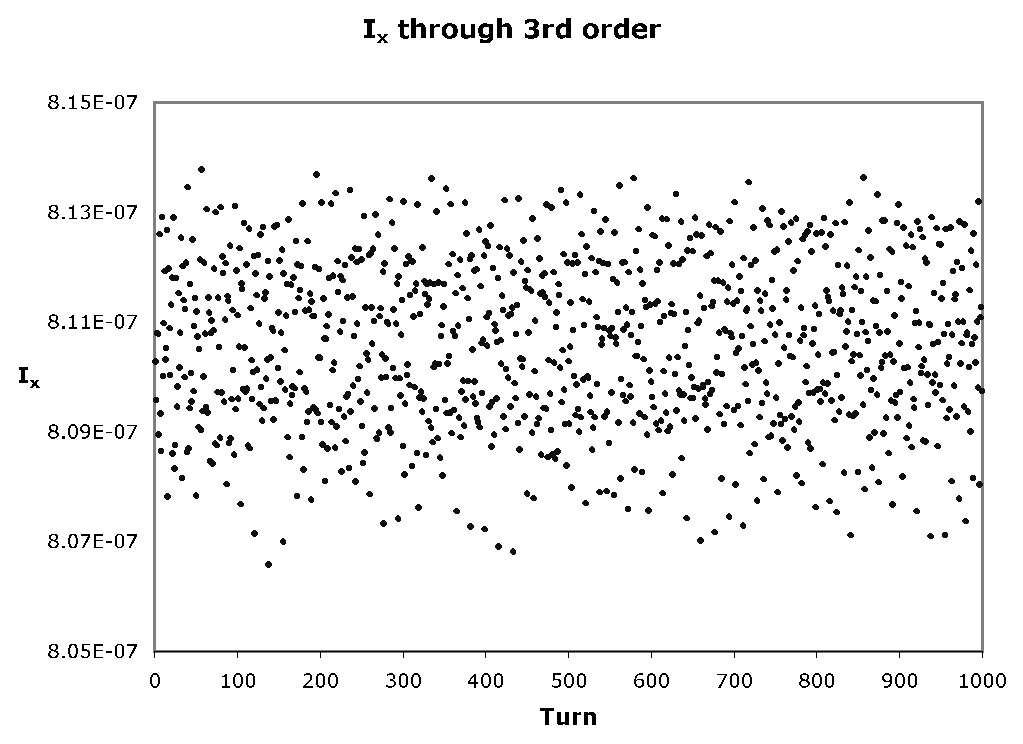
\includegraphics[height=2.85in]{fig8112}
  \caption{Contents of file 16, turn by turn values of $I_x$ through third order.}
\end{figure}

\begin{figure}[htp]
  \centering
  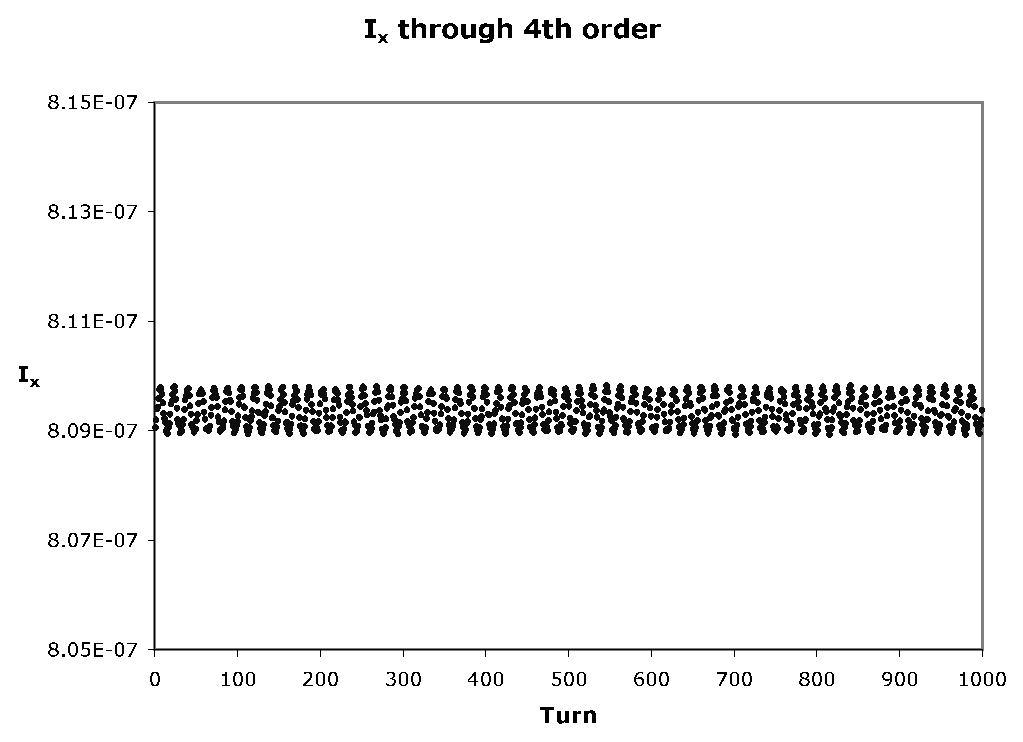
\includegraphics[height=2.85in]{fig8113}
  \caption{Contents of file 16, turn by turn values of $I_x$ through fourth order.}
\end{figure}

\newpage
\section{Compute Power of Static Normal Form}
\begin{quotation}
\noindent     Type Code:  psnf \index{power of static normal form}
\vspace{5mm}

\noindent Required Parameters:
\begin{enumerate}
      \item  JINOPT (controls meaning of the second parameter, POW)

             = 1 if POW is to be interpreted as a power.

             = 2 if POW is to be interpreted as a file number or the number
               of a param- \hspace*{1em}eter set array.

      \item  POW

             = power when JINOPT = 1.

             = NPOWFILE [Number of file from which power(s) is (are) to be
               read when \hspace*{1em}JINOPT = 2].

             Note:  When NPOWFILE = $-$J (with J an integer from 1 to 9),
             powers are taken from the parameter set array associated with
             the type code {\em psj}.  In this case, zero parameter values are
             ignored.


      \item  MAPIN

             = 0 to use current transfer map.

             = NMAP (with NMAP an integer from 1 to 9) to use map in
               storage location \hspace*{1em}NMAP.

      \item  JOUTOPT

             = 0 to place resulting map in a location specified by the
               parameter \linebreak \hspace*{1em}MAPOUT.  If several maps are computed,
               only the last is placed and \hspace*{1em}the rest are lost.

             = NOUTFILE to write resulting map(s) on file NOUTFILE.  In
               this case \hspace*{1em}the parameter MAPOUT is ignored.

      \item  MAPOUT

             = KMAP (with KMAP an integer from 1 to 9) to place resulting
               map in \hspace*{1em}storage location KMAP.

             = 0 to make the resulting map the current transfer map.

             = $-$KBUF (with KBUF an integer from 1 to 6) to place resulting
               map in \hspace*{1em}buffer number KBUF.
\end{enumerate}

\vspace{5mm}
\noindent     Example:
\begin{verbatim}
         powrs    psnf
           1 , 2.5 , 0, 16 , 0
\end{verbatim}
\end{quotation}
This specifies a command with the user given name {\em powrs}.  When invoked it assumes that the current transfer map is in static normal form and raises it to a power (which can be any real number) that in this case is 2.5.

\vspace{5mm}
     Description:
\vspace{2mm}

Suppose ${\cal N}$ is a map that is known to be in static normal form.  This command makes it possible to compute ${\cal N}^s$ where $s$ is any real number.  This command can be useful for producing a filamented phase-space distribution since the normal form can have anharmonic terms.  See also section 8.29.

\vspace{5mm}
%\pagebreak
NOTE WELL:
\vspace{2mm}

     The file NOUTFILE is brought to its end before writing, so that
transfer maps (if any) already on file NOUTFILE are not overwritten.

\newpage
\section{Compute Power of Dynamic Normal Form}
\begin{quotation}
\noindent     Type Code:  pdnf \index{power of dynamic normal form}
\vspace{5mm}

\noindent     Required Parameters:
\begin{enumerate}
      \item  JINOPT (controls meaning of the second parameter, POW)

             = 1 if POW is to be interpreted as a power.

             = 2 if POW is to be interpreted as a file number or the number
               of a param- \hspace*{1em}eter set array.

      \item  POW
             = NPOWFILE [Number of file from which power(s) is (are) to be
               read when JINOPT = 2].

             Note:  If NPOWFILE = $-$J (with J an integer from 1 to 9),
             powers are taken from the parameter set array associated with
             the type code {\em psj}.  In this case, zero parameter values are
             ignored.


      \item  MAPIN

             = 0 to use current transfer map.

             = NMAP (with NMAP an integer from 1 to 9) to use map in
               storage location \hspace*{1em}NMAP.

      \item  JOUTOPT

             = 0 to place resulting map in a location specified by the
           parameter \linebreak \hspace*{1em}MAPOUT\@.  If several maps are computed, only
           the last is placed and \hspace*{1em}the rest are lost.

             = NOUTFILE to write resulting map(s) on file NOUTFILE.  In
               this case \hspace*{1em}the parameter MAPOUT is ignored.

      \item  MAPOUT

             = KMAP (with KMAP an integer from 1 to 9) to place resulting
               map in \hspace*{1em}storage location KMAP.

             = 0 to make the resulting map the current transfer map.

             = $-$KBUF (with KBUF an integer from 1 to 6) to place resulting
               map in \hspace*{1em}buffer number KBUF.
\end{enumerate}

\vspace{5mm}
\noindent Example:
\begin{verbatim}
         powrd    pdnf
           1, 2.5 , 0 , 16 , 0
\end{verbatim}
\end{quotation}
This specifies a command with the user given name {\em powrd}.  When invoked it assumes that the current transfer map is in dynamic normal form and raises it to a power (which can be any real number) that in this case is 2.5.

\vspace{5mm}
     Description:
\vspace{2mm}

Suppose ${\cal N}$ is a map that is known to be in dynamic normal form.  This command makes it possible to compute ${\cal N}^s$ where $s$ is any real number.  This command can be useful for producing a filamented phase-space distribution since the normal form can have anharmonic terms.  See also section 8.29.

\vspace{5mm}
%\pagebreak
NOTE WELL:
\vspace{2mm}

     The file NOUTFILE is brought to its end before writing, so that
transfer maps (if any) already on file NOUTFILE are not overwritten.

\newpage
\section{Get Buffer Contents}\index{get buffer contents} \index{buffers}
\begin{quotation}
\noindent     Type Code:  gbuf
\vspace{5mm}

\noindent Required Parameters:
\begin{enumerate}
      \item  IOPT

             = 1 to concatenate existing map with the map in NBUF.

             = 2 to replace the existing map with the map in NBUF.

      \item  NBUF (an integer from 1 to 6).
\end{enumerate}

\vspace{5mm}
\noindent     Example:
\begin{verbatim}
         getbuf2    gbuf
         1, 2
\end{verbatim}
\end{quotation}
This specifies a command with the user given name {\em getbuf2}.  When invoked it concatenates the current map with the map in buffer 2 and makes the result the current map.

\vspace{5mm}
     Description:
\vspace{2mm}

     Several analysis commands fill various buffers with various maps.  These maps are then available for further use by employing a command with type code {\em gbuf}.

\newpage
\section{Fourier Analyze Static Map}\index{Fourier analyze}
\begin{quotation}
\noindent Type Code:  fasm
\end{quotation}

Not yet available.

\newpage
\section{Fourier Analyze Dynamic Map} \index{Fourier analyze}
\begin{quotation}
\noindent Type Code:  fadm
\end{quotation}

Not yet available.

\newpage
\section{Apply Map to a Function or Moments}\index{apply map} \index{function} \index{moment}
\begin{quotation}
\noindent     Type Code:  amap
\vspace{5mm}

\noindent Required Parameters:
\begin{enumerate}
      \item  JOB

             = 0 to act on a function.

             = 1 to act on initial moments through order 4 and to compute
               transformed \hspace*{1em}moments through $2^{\mbox{\scriptsize nd}}$ moments.

             = 2 to act on initial moments through order 4 and to compute
               transformed \hspace*{1em}moments through $4^{\mbox{\scriptsize th}}$ moments.  (This requires more execution time.)

      \item  ISEND

             = 0 to do nothing.

             = 1 to write transformed function or moments at the terminal.

             = 2 to write transformed function or moments on file 12.

             = 3 to write transformed function or moments at the terminal
			 and on file \hspace*{1em}12.

      \item  NINFILE

             = $-$NMAP to get function or moments from storage location NMAP
			   (see \hspace*{1em}section 7.17).

             = INFILE (file number from which function or moments are to be
               read).

      \item  NREWIND

             = 0 to read (from file INFILE) in its current position.

             = 1 to first rewind file unit INFILE, then read.

      \item  NSKIP

             Number of data sets (functions or moment sets) to be skipped
             in file INFILE (starting from the current position) before a
             read actually occurs.

      \item  NOUTFILE

             = 0 to not write out transformed function or transformed
               moments.

             = NOUTFILE to write transformed function or transformed moment
               set on \hspace*{1em}file NOUTFILE.
\end{enumerate}

\vspace{5mm}
\noindent Example 1:
\begin{verbatim}
         amapf    amap
         0 , 1 , -3 , 0 , 0 , 0
\end{verbatim}
%\end{quotation}
This specifies a command with the user given name {\em amapf}.  When it is invoked the current transfer map ${\cal M}$ acts on the function in storage location 3 and writes the transformed function at the terminal.

\vspace{5mm}
\noindent Example 2:
\begin{verbatim}
         amapm    amap
         2 , 1 , -3 , 0 , 0 , 0
\end{verbatim}
\end{quotation}
This specifies a command with the user given name {\em amapm}.  When it is invoked the current transfer map ${\cal M}$ acts on the set of moments in storage location 3 and writes the transformed moments at the terminal.

Note: \ When {\em amap} takes in moments from a ``map'', it uses the array part of the map and ignores its matrix part.  Note that the zeroth entry $P(0)$ must have the value 1.  See section 4.4.3.

\vspace{5mm}
     Description:
%\begin{quotation}
\vspace{2mm}

Suppose JOB = 0.  Let $f(z)$ be a polynomial function gotten from a storage location or read in from an  external file, and let ${\cal M}$ be the current transfer map.  Then this command computes the transformed function $g(z)$ given by
\begin{equation}
g = {\cal M} f.
\end{equation}

The case of a map acting on moments (JOB = 1 or 2) requires more explanation.  Consider the following gedanken exercise: \ Suppose one is given a collection of particles distributed in phase space.  Their coordinates could be stored, for instance, in the initial conditions buffer.  For this distribution one could find the moments $\langle 1\rangle$, $\langle z_a\rangle$, $\langle z_az_b\rangle$, $\langle z_az_bz_c\rangle$, $\langle z_az_bz_cz_d\rangle$.  This could be done, for example, by use of a {\em bgen} command with JOB = 0.  See section 8.34.  Next, supose ${\cal M}$ is the transfer map describing the system under study.  This map could be applied to all the particles in the phase-space distribution, and this transformed distribution could be used to compute transformed moments.  In this way a set of original moments is sent, under the action of ${\cal M}$, to a set of transformed moments.

With this background in mind, one may wonder if there is a way to compute the action of ${\cal M}$ on moments without tracking (computing the effect of ${\cal M}$ on) thousands or millions of particles, which can be computationally intensive.  The answer is yes.  Let $P_{\alpha}(z)$ with $\alpha = 0,1,2,\cdots 209$ denote a basis monomial as in section 14.1.  Given a phase-space distribution function $f(z)$, one can define associated moments $m_{\alpha}$ by the rule
\begin{equation}
m_{\alpha} = \int d^6z P_{\alpha}(z) f(z).
\end{equation}
For example, we have the definitions
\begin{equation}
m_1 = \int d^6z P_1(z) f(z) = \int d^6z (z_1) f(z) = \langle z_1\rangle ,
\end{equation}
\begin{equation}
m_8 = \int d^6z P_8(z) f(z) = \int d^6z (z_1z_2) f(z) = \langle z_1z_2\rangle , \ {\rm etc}.
\end{equation}
Also, for convenience, the phase-space distribution is normalized to have an integral of one,
\begin{equation}
m_0 = \int d^6z P_0(z) f(z) dz =  \int d^6z(1) f(z) = \langle 1\rangle = 1.
\end{equation}
Under the action of ${\cal M}$ the phase-space distribution function is sent to the {\em transformed} distribution $f^{\rm tr}$ with
\begin{equation}
f^{\rm tr}(z) = f({\cal M}^{-1} z).
\end{equation}
This result is just Liouville's theorem.  Correspondingly, the moments $m_{\alpha}$ are sent to trasformed moments $m^{\rm tr}_{\alpha}$ with
\begin{equation}
m^{\rm tr}_{\alpha} = \int d^6z P_{\alpha}(z) f^{\rm tr}(z).
\end{equation}
Combining (17.6) and (17.7) gives the result
\begin{equation}
m^{\rm tr}_{\alpha} = \int d^6z P_{\alpha}(z) f({\cal M}^{-1} z) = \int d^6z^{\prime} P_{\alpha}({\cal M} z^{\prime}) f(z^{\prime}).
\end{equation}
Here we have made the change of variables
\begin{equation}
z^{\prime} = {\cal M}^{-1} z,
\end{equation}
which has unit Jacobian because ${\cal M}$ is a symplectic map.  Also, since the basis monomials form a complete set, there are relations of the form
\begin{equation}
P_{\alpha} ({\cal M} z^{\prime}) = \sum_{\alpha^{\prime}} {\cal D}_{\alpha \alpha^{\prime}} ({\cal M}) P_{\alpha^{\prime}}(z^{\prime}).
\end{equation}
Finally, insert (17.10) into (17.8) to obtain the result
\begin{equation}
m^{\rm tr}_{\alpha} = \int d^6 z^{\prime}  \sum_{\alpha^{\prime}} {\cal D}_{\alpha \alpha^{\prime}} ({\cal M}) P_{\alpha^{\prime}}(z^{\prime}) f(z^{\prime})
\end{equation}
or
\begin{equation}
m^{\rm tr}_{\alpha} = \sum_{\alpha^{\prime}} {\cal D}_{\alpha \alpha^{\prime}} ({\cal M}) m_{\alpha^{\prime}}.
\end{equation}
We see that moments transform like the components of a vector, and their transformation can be found without tracking provided one  knows the matrix ${\cal D}$.  This is what is done in \Mary when a map ${\cal M}$ is made to act on moments by invoking an {\em amap} command with JOB = 1 or 2.

Since \Mary 3.0 is a third order code, its internal computational machinery has been restricted to work with polynomials of degree 4 and lower.  Correspondingly, there is some truncation in the entries of ${\cal D}$ as listed below.

\begin{center}
                             JOB = 1 or 2

Required Initial Moments:  $\displaystyle \langle 1\rangle , \langle z_a\rangle , \langle z_a z_b\rangle , \langle z_a z_b z_c\rangle , \langle z_a z_b z_c z_d\rangle .$
\end{center}
\[ \begin{array}{lll}
\mbox{\underline{Final Moment}}   & &   \mbox{\underline{Map Employed}}\\
\langle z_a\rangle          & &  \displaystyle    e^{:f_2:}[1+\Lieop(f_3)
+ (\frac{\Lieop(f_3)^2}{2!} + \Lieop(f_4)) + (\frac{\Lieop(f_3)^3}{3!} +
\Lieop(f_3)\Lieop(f_4))]\vspace{1mm}\\
\langle z_a z_b\rangle      & (1)  & \displaystyle e^{:f_2:}[1+\Lieop(f_3) + (\frac{\Lieop(f_3)^2}{2!} + \Lieop(f_4))]\\
\langle z_a z_b z_c\rangle  &  (2)   & e^{:f_2:} [1 + \Lieop(f_3)]\\
\langle z_a z_b z_c z_d\rangle  & (3) &   e^{:f_2:}
\end{array} \]
Remarks:

(1)  Effects of $\Lieop(f_3)^3$ and $\Lieop(f_3) \Lieop(f_4)$ are lost

(2)  Effects of $\Lieop(f_3)^2$ and $\Lieop(f_4)$ are lost.

(3)  All effects of $\Lieop(f_3)$ and $\Lieop(f_4)$ are lost. \\

When {\em amap} is invoked, the contents of buffers 1 through 6 are as follows: \ Buffers 3 through 6 are all empty.  If JOB = 0, buffer 1 contains the identity as its matrix part, and the
transformed function as its array part.  Buffer 2 is empty.  If JOB $>$ 0, buffer 1
contains the transformed second moments as its matrix part, and all the transformed moments
as its array part.  The content of NOUTFILE, if written, is the same as buffer 1.  Buffer 2 contains in its matrix part a matrix whose diagonal
entries are the transformed rms moments $\sqrt{\langle z_az_a\rangle}$ and whose
off-diagonal entries are zero.  The array part of buffer 2 is empty.


The Exhibit below illustrates the use of {\em amap} to cause the current transfer map ${\cal M}$ to act on a function.  For examples of the use of {\em amap} to cause ${\cal M}$ to act on moments, see sections 8.37 and 10.12.

\vspace{5mm}
\begin{footnotesize}
\begin{verbatim}
#comment
 Exhibit 8.17.
 This MaryLie run illustrates the use of the type code
 amap for the small static storage ring of Exhibit 2.5.1.
 It uses sia to compute I_x, and then uses amap to verify
 the relation
   script M I_x = I_x.
#beam
  4.86914813175970
 0.849425847892200
  1.00000000000000
  1.00000000000000
#menu
 drvs     drft
  0.300000000000000
 drs      drft
  0.450000000000000
 drml     drft
   1.48646000000000
 drl      drft
   2.28646000000000
 bend     pbnd
   36.0000000000000      0.000000000000000E+00  0.500000000000000
   1.20000000000000
 hfq      quad
  0.500000000000000       2.72000000000000       1.00000000000000
   1.00000000000000
 hdq      quad
  0.500000000000000      -1.92000000000000       1.00000000000000
   1.00000000000000
 hcs      sext
  0.500000000000000      -1.62000000000000
 vcs      sext
  0.500000000000000       3.34000000000000
 fileout  pmif
   1.00000000000000       12.0000000000000       3.00000000000000
 mapout   ptm
   3.00000000000000       3.00000000000000      0.000000000000000E+00
  0.000000000000000E+00   1.00000000000000
 raysin   rt
   13.0000000000000       14.0000000000000      -1.00000000000000
  0.000000000000000E+00  0.000000000000000E+00  0.000000000000000E+00
 track    rt
   13.0000000000000       14.0000000000000       5.00000000000000
   500.000000000000       1.00000000000000      0.000000000000000E+00
 chrom    tasm
   2.00000000000000      1.000000000000000E-03   1.00000000000000
  0.000000000000000E+00   3.00000000000000      0.000000000000000E+00
 snor     snor
  0.000000000000000E+00   3.00000000000000       3.00000000000000
   1.00000000000000      0.000000000000000E+00
 sia      sia
  0.000000000000000E+00   1.00000000000000      0.000000000000000E+00
   3.00000000000000      0.000000000000000E+00
 amap     amap
  0.000000000000000E+00   1.00000000000000      -3.00000000000000
  0.000000000000000E+00  0.000000000000000E+00  0.000000000000000E+00
 gbuf3    gbuf
   2.00000000000000       3.00000000000000
 stm1     stm
   1.00000000000000
 gtm1     gtm
   2.00000000000000       1.00000000000000
 stm3     stm
   3.00000000000000
 iden     iden
 zer      zer
  0.000000000000000E+00  5.000000000000000E-10  5.000000000000000E-10
  0.000000000000000E+00
 fin      end
#lines
 nsex
     1*drl         1*hdq         1*drs         1*bend        1*drs      &
     1*hfq         1*drl
 tsex
     1*drl         1*hdq         1*drs         1*bend        1*drs      &
     1*hfq         1*drvs        1*hcs         1*drml
 lsex
     1*drml        1*vcs         1*drvs        1*hdq         1*drs      &
     1*bend        1*drs         1*hfq         1*drl
 half
     1*nsex        1*tsex        1*lsex        1*nsex        1*nsex
 ring
     2*half
#lumps
#loops
#labor
    1*fileout
    1*zer
    1*ring
    1*stm1
    1*sia
    1*gbuf3
    1*stm3
    1*gtm1
    1*amap
    1*fin
map stored in location   1

static invariant analysis

x invariant polynomial

nonzero elements in generating polynomial are :

 f(  7)=f( 20 00 00 )= 0.28283741725472
 f(  8)=f( 11 00 00 )=  1.8119521227272
 f( 12)=f( 10 00 01 )=  1.4555083997013
 f( 13)=f( 02 00 00 )=  6.4375945779623
 f( 17)=f( 01 00 01 )=  1.7697319603908
 f( 27)=f( 00 00 02 )=  2.4641432149979
 f( 28)=f( 30 00 00 )= 8.14862086573107E-02
 f( 29)=f( 21 00 00 )=  1.7909382522170
 f( 33)=f( 20 00 01 )= -1.9439421600706
 f( 34)=f( 12 00 00 )=-0.69316455416935
 f( 38)=f( 11 00 01 )=  15.321043502166
 f( 39)=f( 10 20 00 )=  1.1234824876277
 f( 40)=f( 10 11 00 )= -11.278066755118
 f( 43)=f( 10 02 00 )=  28.683783323401
 f( 48)=f( 10 00 02 )= -24.790310322533
 f( 49)=f( 03 00 00 )= -39.498206914693
 f( 53)=f( 02 00 01 )=  97.662016671074
 f( 54)=f( 01 20 00 )=  2.2361389163827
 f( 55)=f( 01 11 00 )= -34.437321940070
 f( 58)=f( 01 02 00 )=  45.847633132341
 f( 63)=f( 01 00 02 )= -70.504642686509
 f( 67)=f( 00 20 01 )=  3.4481379195691
 f( 70)=f( 00 11 01 )= -29.709584450401
 f( 76)=f( 00 02 01 )=  92.634094832153
 f( 83)=f( 00 00 03 )= -34.140122269086
 f( 84)=f( 40 00 00 )= 0.26625964929444
 f( 85)=f( 31 00 00 )= 0.47460012884628
 f( 89)=f( 30 00 01 )= 0.45302042859664
 f( 90)=f( 22 00 00 )= -5.8313785812592
 f( 94)=f( 21 00 01 )= -22.489395096546
 f( 95)=f( 20 20 00 )= -133.94768609570
 f( 96)=f( 20 11 00 )=  716.49307547164
 f( 99)=f( 20 02 00 )=  774.63973894177
 f(104)=f( 20 00 02 )=  15.411106871683
 f(105)=f( 13 00 00 )=  24.170787005918
 f(109)=f( 12 00 01 )= -110.98043731593
 f(110)=f( 11 20 00 )= -729.49630673371
 f(111)=f( 11 11 00 )= -3093.2302592337
 f(114)=f( 11 02 00 )=  26125.403574480
 f(119)=f( 11 00 02 )= -166.56546917394
 f(123)=f( 10 20 01 )= -765.01365459675
 f(126)=f( 10 11 01 )=  7138.4652828102
 f(132)=f( 10 02 01 )= -5514.3389878372
 f(139)=f( 10 00 03 )=  198.38331770005
 f(140)=f( 04 00 00 )=  265.28967521583
 f(144)=f( 03 00 01 )= -598.26336904547
 f(145)=f( 02 20 00 )=  756.61139263247
 f(146)=f( 02 11 00 )= -26007.556806726
 f(149)=f( 02 02 00 )=  64393.054340637
 f(154)=f( 02 00 02 )=  336.51063798049
 f(158)=f( 01 20 01 )= -3530.0340246697
 f(161)=f( 01 11 01 )=  9875.9553103357
 f(167)=f( 01 02 01 )=  49139.325361611
 f(174)=f( 01 00 03 )= -542.28702501823
 f(175)=f( 00 40 00 )=  1.2469479054074
 f(176)=f( 00 31 00 )= -22.724591921870
 f(179)=f( 00 22 00 )=  178.46754108576
 f(184)=f( 00 20 02 )= -798.84747137678
 f(185)=f( 00 13 00 )= -582.86899632005
 f(190)=f( 00 11 02 )=  12419.528107262
 f(195)=f( 00 04 00 )=  877.06223497910
 f(200)=f( 00 02 02 )= -22602.667052125
 f(209)=f( 00 00 04 )=  601.98597677505

y invariant polynomial

nonzero elements in generating polynomial are :

 f( 18)=f( 00 20 00 )= 0.28222227408050
 f( 19)=f( 00 11 00 )= -1.7421650477668
 f( 22)=f( 00 02 00 )=  6.2319133709247
 f( 39)=f( 10 20 00 )= 0.53664356643599
 f( 40)=f( 10 11 00 )=  2.5453610401654
 f( 43)=f( 10 02 00 )= -19.706225365361
 f( 54)=f( 01 20 00 )= -2.6143765122715
 f( 55)=f( 01 11 00 )=  15.887396574912
 f( 58)=f( 01 02 00 )=  8.6929156992971
 f( 67)=f( 00 20 01 )=  6.1183153892148
 f( 70)=f( 00 11 01 )=  4.5958685600997
 f( 76)=f( 00 02 01 )= -149.28726800044
 f( 95)=f( 20 20 00 )=  137.21682431703
 f( 96)=f( 20 11 00 )= -728.58802024760
 f( 99)=f( 20 02 00 )= -737.95782611400
 f(110)=f( 11 20 00 )=  740.24779668774
 f(111)=f( 11 11 00 )=  3047.6089348420
 f(114)=f( 11 02 00 )= -25879.757217720
 f(123)=f( 10 20 01 )=  780.09330458197
 f(126)=f( 10 11 01 )= -7283.0744155013
 f(132)=f( 10 02 01 )=  5985.4133761219
 f(145)=f( 02 20 00 )= -681.33686819601
 f(146)=f( 02 11 00 )=  25448.466733518
 f(149)=f( 02 02 00 )= -63197.894117966
 f(158)=f( 01 20 01 )=  3510.3583312332
 f(161)=f( 01 11 01 )= -9585.0333015133
 f(167)=f( 01 02 01 )= -49371.953367217
 f(175)=f( 00 40 00 )= 0.92791989651083
 f(176)=f( 00 31 00 )=  3.8316189898871
 f(179)=f( 00 22 00 )= -106.96761937402
 f(184)=f( 00 20 02 )=  817.97580713121
 f(185)=f( 00 13 00 )=  412.43621376403
 f(190)=f( 00 11 02 )= -13167.703659685
 f(195)=f( 00 04 00 )= -632.44363424370
 f(200)=f( 00 02 02 )=  25835.201289497
map stored in location   3
map gotten from location   1
map gotten from location   3

 transformed function

nonzero elements in generating polynomial are :

 f(  7)=f( 20 00 00 )= 0.28283741725472
 f(  8)=f( 11 00 00 )=  1.8119521227272
 f( 12)=f( 10 00 01 )=  1.4555083997013
 f( 13)=f( 02 00 00 )=  6.4375945779624
 f( 17)=f( 01 00 01 )=  1.7697319603908
 f( 27)=f( 00 00 02 )=  2.4641432149979
 f( 28)=f( 30 00 00 )= 8.14862086573105E-02
 f( 29)=f( 21 00 00 )=  1.7909382522170
 f( 33)=f( 20 00 01 )= -1.9439421600706
 f( 34)=f( 12 00 00 )=-0.69316455416941
 f( 38)=f( 11 00 01 )=  15.321043502166
 f( 39)=f( 10 20 00 )=  1.1234824876277
 f( 40)=f( 10 11 00 )= -11.278066755118
 f( 43)=f( 10 02 00 )=  28.683783323402
 f( 48)=f( 10 00 02 )= -24.790310322533
 f( 49)=f( 03 00 00 )= -39.498206914693
 f( 53)=f( 02 00 01 )=  97.662016671074
 f( 54)=f( 01 20 00 )=  2.2361389163827
 f( 55)=f( 01 11 00 )= -34.437321940070
 f( 58)=f( 01 02 00 )=  45.847633132341
 f( 63)=f( 01 00 02 )= -70.504642686509
 f( 67)=f( 00 20 01 )=  3.4481379195691
 f( 70)=f( 00 11 01 )= -29.709584450401
 f( 76)=f( 00 02 01 )=  92.634094832153
 f( 83)=f( 00 00 03 )= -34.140122269086
 f( 84)=f( 40 00 00 )= 0.26625964929447
 f( 85)=f( 31 00 00 )= 0.47460012884679
 f( 89)=f( 30 00 01 )= 0.45302042859695
 f( 90)=f( 22 00 00 )= -5.8313785812583
 f( 94)=f( 21 00 01 )= -22.489395096541
 f( 95)=f( 20 20 00 )= -133.94768609570
 f( 96)=f( 20 11 00 )=  716.49307547149
 f( 99)=f( 20 02 00 )=  774.63973894216
 f(104)=f( 20 00 02 )=  15.411106871684
 f(105)=f( 13 00 00 )=  24.170787005911
 f(109)=f( 12 00 01 )= -110.98043731592
 f(110)=f( 11 20 00 )= -729.49630673357
 f(111)=f( 11 11 00 )= -3093.2302592353
 f(114)=f( 11 02 00 )=  26125.403574482
 f(119)=f( 11 00 02 )= -166.56546917392
 f(123)=f( 10 20 01 )= -765.01365459680
 f(126)=f( 10 11 01 )=  7138.4652828097
 f(132)=f( 10 02 01 )= -5514.3389878349
 f(139)=f( 10 00 03 )=  198.38331770005
 f(140)=f( 04 00 00 )=  265.28967521582
 f(144)=f( 03 00 01 )= -598.26336904547
 f(145)=f( 02 20 00 )=  756.61139263289
 f(146)=f( 02 11 00 )= -26007.556806728
 f(149)=f( 02 02 00 )=  64393.054340634
 f(154)=f( 02 00 02 )=  336.51063798053
 f(158)=f( 01 20 01 )= -3530.0340246695
 f(161)=f( 01 11 01 )=  9875.9553103310
 f(167)=f( 01 02 01 )=  49139.325361620
 f(174)=f( 01 00 03 )= -542.28702501822
 f(175)=f( 00 40 00 )=  1.2469479054074
 f(176)=f( 00 31 00 )= -22.724591921871
 f(179)=f( 00 22 00 )=  178.46754108576
 f(184)=f( 00 20 02 )= -798.84747137692
 f(185)=f( 00 13 00 )= -582.86899632005
 f(190)=f( 00 11 02 )=  12419.528107262
 f(195)=f( 00 04 00 )=  877.06223497910
 f(200)=f( 00 02 02 )= -22602.667052123
 f(209)=f( 00 00 04 )=  601.98597677505

end of MARYLIE run
\end{verbatim}
\end{footnotesize}

\newpage
\section{Multiply a Polynomial by a Scalar} \index{scalar multiplication} \index{polynomial}
\begin{quotation}
\noindent     Type Code:  smul
\vspace{5mm}

\noindent Required Parameters:
\begin{enumerate}
      \item  SCALAR

      \item  MAPIN

             = 0 to use current transfer map.

             = NMAP (with NMAP an integer from 1 to 9) to use polynomial in
               storage \hspace*{1em} location NMAP.

      \item  MAPOUT

             = KMAP (with KMAP an integer from 1 to 9) to place resulting
               polynomial \hspace*{1em}in storage location KMAP.

             = 0 to make the resulting polynomial the polynomial  for the current transfer \hspace*{1em}map.

             = $-$KBUF (with KBUF an integer from 1 to 6) to place resulting
               polynomial \hspace*{1em} in buffer number KBUF.

\end{enumerate}

\vspace{5mm}
\noindent Example:
\begin{verbatim}
         stimesp    smul
           3.2 , 1 , 2
\end{verbatim}
\end{quotation}
This specifies a command with the user given name {\em stimesp}.  When invoked, it multiplies the polynomial associated with the map in storage location 1 by the number (3.2), and puts the result in storage location 2.

\vspace{5mm}
     Description:
\vspace{2mm}

This command makes it possible to multiply a polynomial $f$ by a scalar $\lambda$.

\newpage
\section{Add Two Polynomials}\index{add} \index{polynomial}
\begin{quotation}
\noindent     Type Code:  padd
\vspace{5mm}

\noindent Required Parameters:
\begin{enumerate}
      \item  SCAL1

	  \item  SCAL2

      \item  MAP1IN

             = 0 to use current transfer map.

             = NMAP1 (with NMAP1 an integer from 1 to 9) to use polynomial in
               \hspace*{1em}storage location NMAP1.

      \item  MAP2IN

             = 0 to use current transfer map.

             = NMAP2 (with NMAP2 an integer from 1 to 9) to use polynomial in
               \hspace*{1em} storage location NMAP2.

      \item  MAPOUT

             = KMAP (with KMAP an integer from 1 to 9) to place resulting
               polynomial \hspace*{1em}in storage location KMAP.

             = 0 to make the resulting polynomial the polynomial for the current transfer \hspace*{1em}map.

             = $-$KBUF (with KBUF an integer from 1 to 6) to place resulting
               polynomial \hspace*{1em}in buffer number KBUF.
\end{enumerate}

\vspace{5mm}
\noindent Example:
\begin{verbatim}
         p1+p2    padd
        1 , 1 , 1 , 2 , 0
\end{verbatim}
\end{quotation}
This specifies a command with the user given name {\em p1+p2}.  When invoked, it takes the polynomials stored in location 1 and 2, adds them, and makes the result the polynomial entry in the current map.

\vspace{5mm}
     Description:
\vspace{2mm}

Given two scalars $\lambda$, $\mu$ and two polymonials $f,g$ this command makes it possible to compute and store the polynomial $(\lambda f + \mu g)$.

\newpage
\section{Multiply Two Polynomials}\index{polynomial} \index{multiply}
\begin{quotation}
\noindent     Type Code:  pmul
\vspace{5mm}

\noindent     Required Parameters:
\begin{enumerate}
      \item  MAP1IN

             = 0 to use current transfer map.

             = NMAP1 (with NMAP1 an integer from 1 to 9) to use polynomial in
               \hspace*{1em} storage location NMAP1.

      \item  MAP2IN

             = 0 to use current transfer map.

             = NMAP2 (with NMAP2 an integer from 1 to 9) to use polynomial in
               \hspace*{1em} storage location NMAP2.

      \item  MAPOUT

             = KMAP (with KMAP an integer from 1 to 9) to place resulting
               polynomial \hspace*{1em}in storage location KMAP.

             = 0 to make the resulting polynomial the polynomial for the current transfer \hspace*{1em}map.

             = $-$KBUF (with KBUF an integer from 1 to 6) to place resulting
               polynomial \hspace*{1em}in buffer number KBUF.
\end{enumerate}

\vspace{5mm}
\noindent Example:
\begin{verbatim}
         p1xp2     pmul
            1 ,  2 ,  0
\end{verbatim}
\end{quotation}
This specifies a command with user given name {\em p1xp2}.  When invoked, it takes the polynomials stored in locations 1 and 2, multiplies them, and makes the result the polynomial entry in the current map.

\vspace{5mm}
     Description:
\vspace{2mm}

Given two polynomials $f,g$ this command makes it possible to compute and store the polynomial $fg$.

\newpage
\section{Poisson Bracket Two Polynomials}\index{Poisson bracket} \index{polynomial}
\begin{quotation}
\noindent     Type Code:  pb
\vspace{5mm}

\noindent Required Parameters:
\begin{enumerate}
      \item  MAP1IN

             = 0 to use current transfer map.

             = NMAP1 (with NMAP1 an integer from 1 to 9) to use polynomial in
               \hspace*{1em} storage location NMAP1.

      \item  MAP2IN

             = 0 to use current transfer map.

             = NMAP2 (with NMAP2 an integer from 1 to 9) to use polynomial in
               \hspace*{1em} storage location NMAP2.

      \item  MAPOUT

             = KMAP (with KMAP an integer from 1 to 9) to place resulting
               polynomial \hspace*{1em}in storage location KMAP.

             = 0 to make the resulting polynomial the polynomial for the current transfer \hspace*{1em}map.

             = $-$KBUF (with KBUF an integer from 1 to 6) to place resulting
               polynomial \hspace*{1em}in buffer number KBUF.
\end{enumerate}

\vspace{5mm}
\noindent Example:
\begin{verbatim}
         [p1p2]     pb
            1 ,  2 ,  0
\end{verbatim}
\end{quotation}
This specifies a command with user given name {\em [p1p2]}.  When invoked it takes the polynomials stored in locations 1 and 2, forms their Poisson bracket, and makes the result the polynomial in the current map.

\vspace{5mm}
     Description:
\vspace{2mm}

Given two polynomials $f,g$ this command makes it possible to compute and store the polynomial $[f,g]$.

\newpage
\section{Polar Decomposition of a Map}\index{polar decomposition}
\begin{quotation}
\noindent     Type Code:  pold
\vspace{5mm}

\noindent Required Parameters:
\begin{enumerate}
      \item  MAPIN

             = 0 to use current transfer map.

             = NMAP (with NMAP an integer from 1 to 9) to use map in
               storage location \hspace*{1em}NMAP.

      \item  ISEND

             = 0 to do nothing.

             = 1 to write results at the terminal.

             = 2 to write results on file 12.

             = 3 to write results at the terminal and on file 12.

      \item  IDATA

             = 0 to not put out analysis data.

             = 1 to put out eigenvalues of ${\cal P}$ as a matrix.

             = 2 to put out eigenvectors of ${\cal P}$ as a matrix.

             = 3 to put out eigenvalues and eigenvectors of ${\cal P}$.

      \item  IPMAPS

             = 0 to not put out maps.

             = 1 to put out ${\cal O}$.

             = 2 to put out ${\cal P}$.

             = 3 to put out ${\cal O}$ and ${\cal P}$.

      \item  IWMAPS

             = 0 to not write out maps.

             = IFILE to write maps on file IFILE.
\end{enumerate}

\vspace{5mm}
\noindent Example:
\begin{verbatim}
         polar     pold
          1 , 3 , 1 , 2 , 0
\end{verbatim}
\end{quotation}
This specifies a command with the user given name {\em polar}.  When invoked it takes the map from storage location 1, polar decomposes it, writes the results at the terminal and on file 12, and puts out the map ${\cal P}$.

\vspace{5mm}
     Description:
\vspace{2mm}

     The incoming map, call it ${\cal M}$, is decomposed by a command with the
type code {\em pold } into the product ${\cal M} = e^{:f_2^c:} \ e^{:f_2^a:}
\ e^{:f_3:} \ e^{:f_4:} $.  When this is done,
the following maps are put in the following buffers:
\begin{enumerate}
          \item  Buffer 1 contains ${\cal O} = e^{:f_2^c:}$, the ``orthogonal''
                 part of the map.  Specifically, it contains the matrix
associated with ${\cal O}$ in its matrix part, and $f_2^c$ in its array part.

          \item  Buffer 2 contains ${\cal P} = e^{:f_2^a:}$, the positive definite
symmetric part of the map.  Specifically, it contains the matrix
associated with ${\cal P}$ in its matrix part, and $f_2^a$ in its array part.

          \item  Buffer 3 contains ${\cal C} = e^{:f_3:} \ e^{:f_4:}$, the nonlinear part of the map.

          \item  Buffer 4 contains ${\cal D}$, the eigenvalues of ${\cal P}$ written as a
                 map.  That is, the matrix part of ${\cal D}$ is a diagonal matrix
                 of eigenvalues, and the polynomial array part of ${\cal D}$ is
                 empty.

          \item  Buffer 5 contains ${\cal E}$, the eigenvectors of ${\cal P}$ written as a
                 map.  That is, the matrix part of ${\cal E}$ is the matrix of
                 eigenvectors of the matrix part of ${\cal P}$, the polynomial array
                 part of ${\cal E}$ is empty.

		  \item  Buffer 6 is empty.
\end{enumerate}

Theory: \\

Any symplectic matrix $M$ can be written uniquely in the form
\begin{equation}
M = PO
\end{equation}
where $P$ is symplectic and positive-definite symmetric, and $O$ is symplectic and orthogonal.  This is called orthogonal polar decomposition.  The matrices $P$ and $O$, in turn, can be written in form
\begin{equation}
P = \exp (JS^a),
\end{equation}
\begin{equation}
O = \exp (JS^c).
\end{equation}
Here $S^a$ is a symmetric matrix that {\em anticommutes} with $J$,
\begin{equation}
JS^a + S^aJ = 0,
\end{equation}
and $S^c$ is a symmetric matrix that {\em commutes} with $J$,
\begin{equation}
JS^c - S^cJ = 0.
\end{equation}
Finally, the polynomial $f^a_2$ and $f^c_2$ are defined by the relations
\begin{equation}
f^a_2 = -(1/2) \sum_{de} S^a_{de} z_d z_e,
\end{equation}
\begin{equation}
f^c_2 = -(1/2) \sum_{de} S^c_{de} z_d z_e.
\end{equation}

\newpage
\section{Evaluate a Polynomial}\index{evaluate a polynomial} \index{polynomial}
\begin{quotation}
\noindent Type Code:  pval
\vspace{5mm}

\noindent Required Parameters:
\begin{enumerate}
      \item  MAPIN

             = 0 to use current transfer map.

             = NMAP (with NMAP an integer from 1 through 9) to use map in
               storage \hspace*{1em}location NMAP.

             = $-$NMAP (with NMAP an integer from 1 through 6) to use the map in
               \hspace*{1em}buffer number NMAP.


      \item  IDATAIN

             = 0 to use data in the initial conditions buffer.

             = ICFILE $\geq 1$ to read phase space coordinates from an external
               file with \hspace*{1em}number ICFILE.

             = $-$K (with K an integer from 1 to 9) to read phase space
               coordinates from \hspace*{1em}the parameter set array associated with the
               type code {\em psk}.

        \item  IANS

                     = -1 to not write results.

             = 0 to write results into array part of current map.

             = NBUF (an integer from 1 through 6) to write results into array part of \hspace*{1em}buffer number NBUF.

      \item  IWNUM

             = 0 to not write out numerical data.

             = JFILE to write numerical data on file JFILE.
\end{enumerate}

\vspace{5mm}
\noindent Example:
\begin{verbatim}
         valofp     pval
          0 , 0 , 1 , 20
\end{verbatim}
\end{quotation}
This specifies a command with the user given name {\em valofp}.  When invoked it finds the value(s) of the polynomial associated with the current transfer map for the phase-space point(s) in the initial conditions buffer.  The values are written into buffer 1 and on file 20.

\vspace{5mm}
     Description:
\vspace{2mm}

A command with type code {\em pval} can be used to evaluate a polynomial function of the phase-space variables at any point in phase space.  Such a command can be used, for example, to evaluate invariants.  (See sections 8.10 and 8.11.)  For convenience in plotting, the lines in file JFILE are numbered.  Thus, if the initial conditions buffer contains turn-by-turn phase-space data, the file JFILE will contain the turn number in its first column and the values val(0) through val(4) in the remaining 5 columns.  Here val(0) is the value of the constant term in the polynomial, val(1) is the value of the linear part of the polynomial plus that of the constant part, etc.  Thus val(4) is the cumulative value of all terms through fourth order.

The quantities val(0) through val(4) are also available to be used by fitting and optimization routines.  See sections 9.7 through 9.9.  In this case it is assumed there is only one phase-space point (the last) at which the polynomial is being evaluated.  The quantities val(0) through val(4) are put in array locations 0 through 4 of the current transfer map or of buffer number NBUF.

\vspace{5mm}
NOTE WELL:
\vspace{2mm}

     The initial conditions buffer cannot be empty if a command with the
type code {\em pval } and IDATAIN = 0 is to be executed.  Attempting to do so
results in \Mary program termination accompanied by appropriate messages
at the terminal and file 12.

     If desired, the contents of an external file (file 13 for example) can
be placed in the initial conditions buffer for use by a {\em pval } type command
by executing a command of the kind shown below:
\begin{quotation}
\begin{verbatim}
         putinbuf     rt
         13 , 14 , -1 , 0 , 0 , 0
\end{verbatim}
\end{quotation}
See section 7.2.  This command should precede the command with the type
code {\em pval}.

\newpage
\section{Compute Chromatic Expansion} \index{chromatic expansion}
\begin{quotation}
\noindent Type Code:  cxp
\vspace{5mm}

\noindent Required Parameters:
\begin{enumerate}
        \item  IOPT (controls meaning of the second parameter, EPSILON)

             = 1 if EPSILON = $P_\tau$.

             = 2 if EPSILON = $\delta$.  See section 4.1.2.

      \item  EPSILON (value of expansion parameter).

      \item  MAPIN

           = 0 to use current transfer map.

           = NMAP (with NMAP a positive integer in the range 1 through 9) to use the map in storage location NMAP.

           = $-$NMAP (with NMAP a positive integer in the range 1 through 6) to use the map in buffer number NMAP.
 \end{enumerate}

\vspace{5mm}
\noindent     Example:
\begin{verbatim}
         cxppt    cxp
          1  .001  -3
\end{verbatim}
\end{quotation}
This specifies a command with the user given name {\em cxppt}.  When invoked it makes a chromatic expansion of the map in buffer 3 for the option EPSILON  $= P_{\tau}$ with EPSILON having the value .001.

\vspace{5mm}
     Description:
\vspace{2mm}

Consider a map ${\cal M}$ of the form
\begin{equation}
{\cal M}= e^{:f_2:} e^{:f_3:} e^{:f_4:}
\end{equation}
where $f_2$ contains only terms that are quadratic in the ``geometric'' coordinates or terms that are quadratic in $P_\tau$; $f_3$  contains only terms that are linear in $P_\tau$  (and quadratic in the geometric coordinates) or terms that are cubic in $P_\tau$; $f_4$  contains only terms that are quadratic in $P_\tau$  (and quadratic in the geometric coordinates) or terms that are quartic in $P_\tau$.  The maps ${\cal B}$ and ${\cal A}_b$ produced by {\em cod} and {\em tasm} are of this form.  See sections 8.1 and 8.2.  Such maps, when acting only on transverse variables, are described by a matrix that has a power series expansion in $\epsilon$ (where $ \epsilon = P_{\tau}$ or $\epsilon = \delta)$.  See (8.1.30) and (8.2.26).  A command with type code {\em cxp} produces these expansions.  When executed, the following maps are put in the following buffers:
\begin{enumerate}
\item Buffer 1 contains the $\epsilon$ independent matrix in its matrix part, and zeroes in its polynomial part.
\item Buffer 2 contains the matrix that multiples $\epsilon$ in its matrix part, and zeroes in its polynomial part.
\item Buffer 3 contains the matrix that multiples $\epsilon^2$ in its matrix part, and zeroes in its polynomial part.
\item Buffer 4 contains in its matrix part the sum of the terms described above multiplied by their appropriate powers of $\epsilon$ and evaluated for the specified value of $\epsilon$.  Its polynomial part contains zeroes.
\item Buffer 5 is left unchanged.
\item Buffer 6 is left unchanged.
\end{enumerate}

As described in sections 8.1 and 8.2, such expansions are produced by {\em cod} and {\em tasm} for visual inspection, but they are not then available for fitting or optimizing or scanning, etc.  Since {\em cxp} computes and puts these expansions in buffers, they then become so available.  The Exhibit below illustrates, for example, how a {\em tasm} command followed by a {\em cxp} command produces the desired expansions in buffers.

\vspace{5mm}
\begin{footnotesize}
\begin{verbatim}
#comment
 Exhibit 8.24.
 This is a test of the type code cxp.  A command with type
 code tasm is applied to the one-turn map for the small static
 storage ring of Exhibit 2.5.1 to compute an eigenvector expansion.
 Next, the chromatic expansion for script A_b, the normalizing map for
 the betatron factor, is found using a cxp command, and the result
 is seen to agree with the eigenvector expansion.  Both options
 of tasm and cxp are illustrated.
#beam
  4.86914813175970
 0.849425847892200
  1.00000000000000
  1.00000000000000
#menu
 cxppt    cxp
   1.00000000000000      1.000000000000000E-03  -3.00000000000000
 cxpd     cxp
   2.00000000000000     -1.188970448993188E-03  -3.00000000000000
 drvs     drft
  0.300000000000000
 drs      drft
  0.450000000000000
 drml     drft
   1.48646000000000
 drl      drft
   2.28646000000000
 bend     pbnd
   36.0000000000000      0.000000000000000E+00  0.500000000000000
   1.20000000000000
 hfq      quad
  0.500000000000000       2.72000000000000      0.000000000000000E+00
  0.000000000000000E+00
 hdq      quad
  0.500000000000000      -1.92000000000000      0.000000000000000E+00
  0.000000000000000E+00
 hcs      sext
  0.500000000000000      0.000000000000000E+00
 vcs      sext
  0.500000000000000      0.000000000000000E+00
 fileout  pmif
   1.00000000000000       12.0000000000000       3.00000000000000
 mapout   ptm
   3.00000000000000       3.00000000000000      0.000000000000000E+00
  0.000000000000000E+00   1.00000000000000
 tasmpt   tasm
   1.00000000000000       1.00000000000000       3.00000000000000
  0.000000000000000E+00   3.00000000000000      0.000000000000000E+00
 tasmd    tasm
   2.00000000000000       1.00000000000000       3.00000000000000
  0.000000000000000E+00   3.00000000000000      0.000000000000000E+00
 ptdata   ps1
  1.000000000000000E-02  0.000000000000000E+00  1.000000000000000E-02
  0.000000000000000E+00  0.000000000000000E+00  1.000000000000000E-03
 ddata    ps1
  1.000000000000000E-02  0.000000000000000E+00  1.000000000000000E-02
  0.000000000000000E+00  0.000000000000000E+00 -1.188970448993188E-03
 clear    iden
 zer      zer
  0.000000000000000E+00  1.000000000000000E-10  1.000000000000000E-10
  0.000000000000000E+00
 gbuf1    gbuf
   2.00000000000000       1.00000000000000
 gbuf2    gbuf
   2.00000000000000       2.00000000000000
 gbuf3    gbuf
   2.00000000000000       3.00000000000000
 gbuf4    gbuf
   2.00000000000000       4.00000000000000
 fin      end
#lines
 nsex
     1*drl         1*hdq         1*drs         1*bend        1*drs      &
     1*hfq         1*drl
 tsex
     1*drl         1*hdq         1*drs         1*bend        1*drs      &
     1*hfq         1*drvs        1*hcs         1*drml
 lsex
     1*drml        1*vcs         1*drvs        1*hdq         1*drs      &
     1*bend        1*drs         1*hfq         1*drl
 half
     1*nsex        1*tsex        1*lsex        1*nsex        1*nsex
 ring
     2*half
 pttest
     1*ring        1*ptdata      1*tasmpt      1*cxppt       1*writeout
 dtest
     1*ring        1*ddata       1*tasmd       1*cxpd        1*writeout
 writeout
     1*gbuf1       1*mapout      1*gbuf2       1*mapout      1*gbuf3    &
     1*mapout      1*gbuf4       1*mapout
#lumps
#loops
#labor
    1*fileout
    1*pttest
    1*clear
    1*dtest
    1*fin

twiss analysis of static map
 P sub tau =   1.000000000000000E-003
 delta =  -1.188970448993188E-003


eigenvector expansion for epsilon defined in terms of P sub tau:

on energy matrix of eigenvectors

matrix for map is :

 2.53724E+00  6.93889E-18  0.00000E+00  0.00000E+00  0.00000E+00  0.00000E+00
-3.57071E-01  3.94129E-01  0.00000E+00  0.00000E+00  0.00000E+00  0.00000E+00
 0.00000E+00  0.00000E+00  2.49638E+00  0.00000E+00  0.00000E+00  0.00000E+00
 0.00000E+00  0.00000E+00  3.48938E-01  4.00580E-01  0.00000E+00  0.00000E+00
 0.00000E+00  0.00000E+00  0.00000E+00  0.00000E+00  1.00000E+00  0.00000E+00
 0.00000E+00  0.00000E+00  0.00000E+00  0.00000E+00  0.00000E+00  1.00000E+00


epsilon correction

matrix for map is :

 4.73207E-01  4.56623E-01  0.00000E+00  0.00000E+00  0.00000E+00  0.00000E+00
 4.33537E-03 -1.37768E-01  0.00000E+00  0.00000E+00  0.00000E+00  0.00000E+00
 0.00000E+00  0.00000E+00 -3.51450E-01  9.07617E-02  0.00000E+00  0.00000E+00
 0.00000E+00  0.00000E+00 -3.45609E-02  6.90817E-02  0.00000E+00  0.00000E+00
 0.00000E+00  0.00000E+00  0.00000E+00  0.00000E+00  0.00000E+00  0.00000E+00
 0.00000E+00  0.00000E+00  0.00000E+00  0.00000E+00  0.00000E+00  0.00000E+00


epsilon**2 correction

matrix for map is :

 8.13029E-01  5.87798E-02  0.00000E+00  0.00000E+00  0.00000E+00  0.00000E+00
-1.05289E-01 -1.08092E-01  0.00000E+00  0.00000E+00  0.00000E+00  0.00000E+00
 0.00000E+00  0.00000E+00 -5.00009E-01  9.47381E-01  0.00000E+00  0.00000E+00
 0.00000E+00  0.00000E+00  8.21307E-02  2.21126E-01  0.00000E+00  0.00000E+00
 0.00000E+00  0.00000E+00  0.00000E+00  0.00000E+00  0.00000E+00  0.00000E+00
 0.00000E+00  0.00000E+00  0.00000E+00  0.00000E+00  0.00000E+00  0.00000E+00


matrix of eigenvectors when epsilon=  0.10000000D-02

matrix for map is :

 2.53772E+00  4.56682E-04  0.00000E+00  0.00000E+00  0.00000E+00  0.00000E+00
-3.57067E-01  3.93991E-01  0.00000E+00  0.00000E+00  0.00000E+00  0.00000E+00
 0.00000E+00  0.00000E+00  2.49603E+00  9.17091E-05  0.00000E+00  0.00000E+00
 0.00000E+00  0.00000E+00  3.48904E-01  4.00649E-01  0.00000E+00  0.00000E+00
 0.00000E+00  0.00000E+00  0.00000E+00  0.00000E+00  1.00000E+00  0.00000E+00
 0.00000E+00  0.00000E+00  0.00000E+00  0.00000E+00  0.00000E+00  1.00000E+00

matrix for map is :

 2.53724E+00  6.93889E-18  0.00000E+00  0.00000E+00  0.00000E+00  0.00000E+00
-3.57071E-01  3.94129E-01  0.00000E+00  0.00000E+00  0.00000E+00  0.00000E+00
 0.00000E+00  0.00000E+00  2.49638E+00  0.00000E+00  0.00000E+00  0.00000E+00
 0.00000E+00  0.00000E+00  3.48938E-01  4.00580E-01  0.00000E+00  0.00000E+00
 0.00000E+00  0.00000E+00  0.00000E+00  0.00000E+00  1.00000E+00  0.00000E+00
 0.00000E+00  0.00000E+00  0.00000E+00  0.00000E+00  0.00000E+00  1.00000E+00

nonzero elements in generating polynomial are :


matrix for map is :

 4.73207E-01  4.56623E-01  0.00000E+00  0.00000E+00  0.00000E+00  0.00000E+00
 4.33537E-03 -1.37768E-01  0.00000E+00  0.00000E+00  0.00000E+00  0.00000E+00
 0.00000E+00  0.00000E+00 -3.51450E-01  9.07617E-02  0.00000E+00  0.00000E+00
 0.00000E+00  0.00000E+00 -3.45609E-02  6.90817E-02  0.00000E+00  0.00000E+00
 0.00000E+00  0.00000E+00  0.00000E+00  0.00000E+00  0.00000E+00  0.00000E+00
 0.00000E+00  0.00000E+00  0.00000E+00  0.00000E+00  0.00000E+00  0.00000E+00

nonzero elements in generating polynomial are :


matrix for map is :

 8.13029E-01  5.87798E-02  0.00000E+00  0.00000E+00  0.00000E+00  0.00000E+00
-1.05289E-01 -1.08092E-01  0.00000E+00  0.00000E+00  0.00000E+00  0.00000E+00
 0.00000E+00  0.00000E+00 -5.00009E-01  9.47381E-01  0.00000E+00  0.00000E+00
 0.00000E+00  0.00000E+00  8.21307E-02  2.21126E-01  0.00000E+00  0.00000E+00
 0.00000E+00  0.00000E+00  0.00000E+00  0.00000E+00  0.00000E+00  0.00000E+00
 0.00000E+00  0.00000E+00  0.00000E+00  0.00000E+00  0.00000E+00  0.00000E+00

nonzero elements in generating polynomial are :


matrix for map is :

 2.53772E+00  4.56682E-04  0.00000E+00  0.00000E+00  0.00000E+00  0.00000E+00
-3.57067E-01  3.93991E-01  0.00000E+00  0.00000E+00  0.00000E+00  0.00000E+00
 0.00000E+00  0.00000E+00  2.49603E+00  9.17091E-05  0.00000E+00  0.00000E+00
 0.00000E+00  0.00000E+00  3.48904E-01  4.00649E-01  0.00000E+00  0.00000E+00
 0.00000E+00  0.00000E+00  0.00000E+00  0.00000E+00  1.00000E+00  0.00000E+00
 0.00000E+00  0.00000E+00  0.00000E+00  0.00000E+00  0.00000E+00  1.00000E+00

nonzero elements in generating polynomial are :


twiss analysis of static map
 P sub tau =   1.000000000000000E-003
 delta =  -1.188970448993188E-003


eigenvector expansion for epsilon defined in terms of momentum deviation:

on momentum matrix of eigenvectors

matrix for map is :

 2.53724E+00  6.93889E-18  0.00000E+00  0.00000E+00  0.00000E+00  0.00000E+00
-3.57071E-01  3.94129E-01  0.00000E+00  0.00000E+00  0.00000E+00  0.00000E+00
 0.00000E+00  0.00000E+00  2.49638E+00  0.00000E+00  0.00000E+00  0.00000E+00
 0.00000E+00  0.00000E+00  3.48938E-01  4.00580E-01  0.00000E+00  0.00000E+00
 0.00000E+00  0.00000E+00  0.00000E+00  0.00000E+00  1.00000E+00  0.00000E+00
 0.00000E+00  0.00000E+00  0.00000E+00  0.00000E+00  0.00000E+00  1.00000E+00


epsilon correction

matrix for map is :

-3.98066E-01 -3.84116E-01  0.00000E+00  0.00000E+00  0.00000E+00  0.00000E+00
-3.64696E-03  1.15892E-01  0.00000E+00  0.00000E+00  0.00000E+00  0.00000E+00
 0.00000E+00  0.00000E+00  2.95644E-01 -7.63497E-02  0.00000E+00  0.00000E+00
 0.00000E+00  0.00000E+00  2.90730E-02 -5.81122E-02  0.00000E+00  0.00000E+00
 0.00000E+00  0.00000E+00  0.00000E+00  0.00000E+00  0.00000E+00  0.00000E+00
 0.00000E+00  0.00000E+00  0.00000E+00  0.00000E+00  0.00000E+00  0.00000E+00


epsilon**2 correction

matrix for map is :

 5.17137E-01 -1.45565E-02  0.00000E+00  0.00000E+00  0.00000E+00  0.00000E+00
-7.50390E-02 -5.95479E-02  0.00000E+00  0.00000E+00  0.00000E+00  0.00000E+00
 0.00000E+00  0.00000E+00 -3.10606E-01  6.59239E-01  0.00000E+00  0.00000E+00
 0.00000E+00  0.00000E+00  6.23685E-02  1.47981E-01  0.00000E+00  0.00000E+00
 0.00000E+00  0.00000E+00  0.00000E+00  0.00000E+00  0.00000E+00  0.00000E+00
 0.00000E+00  0.00000E+00  0.00000E+00  0.00000E+00  0.00000E+00  0.00000E+00


matrix of eigenvectors when epsilon= -0.11889704D-02

matrix for map is :

 2.53772E+00  4.56682E-04  0.00000E+00  0.00000E+00  0.00000E+00  0.00000E+00
-3.57067E-01  3.93991E-01  0.00000E+00  0.00000E+00  0.00000E+00  0.00000E+00
 0.00000E+00  0.00000E+00  2.49603E+00  9.17094E-05  0.00000E+00  0.00000E+00
 0.00000E+00  0.00000E+00  3.48904E-01  4.00649E-01  0.00000E+00  0.00000E+00
 0.00000E+00  0.00000E+00  0.00000E+00  0.00000E+00  1.00000E+00  0.00000E+00
 0.00000E+00  0.00000E+00  0.00000E+00  0.00000E+00  0.00000E+00  1.00000E+00

matrix for map is :

 2.53724E+00  6.93889E-18  0.00000E+00  0.00000E+00  0.00000E+00  0.00000E+00
-3.57071E-01  3.94129E-01  0.00000E+00  0.00000E+00  0.00000E+00  0.00000E+00
 0.00000E+00  0.00000E+00  2.49638E+00  0.00000E+00  0.00000E+00  0.00000E+00
 0.00000E+00  0.00000E+00  3.48938E-01  4.00580E-01  0.00000E+00  0.00000E+00
 0.00000E+00  0.00000E+00  0.00000E+00  0.00000E+00  1.00000E+00  0.00000E+00
 0.00000E+00  0.00000E+00  0.00000E+00  0.00000E+00  0.00000E+00  1.00000E+00

nonzero elements in generating polynomial are :


matrix for map is :

-3.98066E-01 -3.84116E-01  0.00000E+00  0.00000E+00  0.00000E+00  0.00000E+00
-3.64696E-03  1.15892E-01  0.00000E+00  0.00000E+00  0.00000E+00  0.00000E+00
 0.00000E+00  0.00000E+00  2.95644E-01 -7.63497E-02  0.00000E+00  0.00000E+00
 0.00000E+00  0.00000E+00  2.90730E-02 -5.81122E-02  0.00000E+00  0.00000E+00
 0.00000E+00  0.00000E+00  0.00000E+00  0.00000E+00  0.00000E+00  0.00000E+00
 0.00000E+00  0.00000E+00  0.00000E+00  0.00000E+00  0.00000E+00  0.00000E+00

nonzero elements in generating polynomial are :


matrix for map is :

 5.17137E-01 -1.45565E-02  0.00000E+00  0.00000E+00  0.00000E+00  0.00000E+00
-7.50390E-02 -5.95479E-02  0.00000E+00  0.00000E+00  0.00000E+00  0.00000E+00
 0.00000E+00  0.00000E+00 -3.10606E-01  6.59239E-01  0.00000E+00  0.00000E+00
 0.00000E+00  0.00000E+00  6.23685E-02  1.47981E-01  0.00000E+00  0.00000E+00
 0.00000E+00  0.00000E+00  0.00000E+00  0.00000E+00  0.00000E+00  0.00000E+00
 0.00000E+00  0.00000E+00  0.00000E+00  0.00000E+00  0.00000E+00  0.00000E+00

nonzero elements in generating polynomial are :


matrix for map is :

 2.53772E+00  4.56682E-04  0.00000E+00  0.00000E+00  0.00000E+00  0.00000E+00
-3.57067E-01  3.93991E-01  0.00000E+00  0.00000E+00  0.00000E+00  0.00000E+00
 0.00000E+00  0.00000E+00  2.49603E+00  9.17094E-05  0.00000E+00  0.00000E+00
 0.00000E+00  0.00000E+00  3.48904E-01  4.00649E-01  0.00000E+00  0.00000E+00
 0.00000E+00  0.00000E+00  0.00000E+00  0.00000E+00  1.00000E+00  0.00000E+00
 0.00000E+00  0.00000E+00  0.00000E+00  0.00000E+00  0.00000E+00  1.00000E+00

nonzero elements in generating polynomial are :


end of MARYLIE run
\end{verbatim}
\end{footnotesize}

\newpage
\section{Transfer Quadratic Moments} \index{transfer quadratic moments} \index{quadratic moments} \index{moment}
\begin{quotation}
\noindent Type Code:  tqm
\vspace{5mm}

\noindent Required Parameters:
\begin{enumerate}
       \item  JOB

              = 1 to use array part of map as source of 2nd moments, and to set matrix \hspace*{1em}part accordingly.

              = 2 to use matrix part of map as source of 2nd moments, and to set array \hspace*{1em}part accordingly.
       \item  IMAP

              = 0 to carry out this ``transfer'' on the current map.

              = NBUF (an integer from 1 through 6) to carry out this ``transfer'' on the \hspace*{1em}map in buffer number NBUF.

\end{enumerate}

\vspace{5mm}
\noindent Example:
\begin{verbatim}
          setmat     tqm
            1         2
\end{verbatim}
\end{quotation}
This specifies a command with the user name {\em setmat}.  When invoked it uses the array part of buffer 2, locations 7 through 27 (see section 14.1), as a source of 2nd moments and sets the matrix part accordingly so that
\[
r1(i,j) = \langle z_iz_j\rangle
\]
where r1 is the matrix part of buffer 1.

\vspace{5mm}
     Description:
\vspace{2mm}

When beam moments are stored in map format, it is usually the case that the array part of the map contains all moments from zero through fourth order, and the matrix part contains 2nd order moments.  However, it may happen that the matrix part contains something else, and it is desired that it contain 2nd moments.  This can be achieved by executing a command with type code {\em tqm} and JOB = 1.  See the example above and section 8.37.  One could also imagine a circumstance in which 2nd moments are specified in matrix form, and it would be desirable to have them in the array part of a map so they could be acted on by {\em amap} or analyzed by {\em moma}.  See sections 8.17 and 8.37.  This can be achieved by executing a {\em tqm} command with JOB = 2.


\newpage
\section{Select Quantities} \index{select quantities} \index{quantities}
\begin{quotation}
\noindent     Type Code:  sq
\vspace{5mm}

\noindent Required Parameters:
\begin{enumerate}
       \item  INFILE (File number from which selections are to be read).

              = 0 or 5 to read interactively from the terminal.

              = IFILE (any positive integer) to read from that file,
after rewinding that \hspace*{1em}file.

              = $-$IFILE (any negative integer) to read from file IFILE at
its current \hspace*{1em}position without rewinding.

       \item  LOGFILE (File number to which selections are to be written.  Ignored unless INFILE = 0 or 5, but still required.)

              = 0 to not write out selections.

              = JFILE (any positive integer) to write selections to that file.


       \item  ISTORE

	          = 1 to put selections in storage associated with inner
			  procedure.

	          = 2 to put selections in storage associated with outer
			  procedure.

	          = 3 to put selections in auxiliary storage.



       \item  ISEND (Ignored, but still required, when INFILE = 0 or 5).

              = 0 to write out nothing.

              = 1 to write out selections at the terminal.

              = 2 to write out selections on file 12.

              = 3 to write out selections at the terminal and on file 12.
\end{enumerate}

\vspace{5mm}
\noindent Example:
\begin{verbatim}
          choices     sq
             25, 0, 3, 1
\end{verbatim}
\end{quotation}
This specifies a command with the user name {\em choices}.  When invoked it reads selections from file 25, puts them in auxiliary storage, and writes them at the terminal.

\vspace{5mm}
     Description:
\vspace{2mm}

This command is used in conjunction with the {\em wsq} command.  See section 8.27.  It is used to select various parameters used by \Mary and various quantities computed by \Mary.  See, for example, section 10.9.  If desired, it may be employed interactively by setting INFILE = 5.  The results of an interactive use may be written on LOGFILE for subsequent noninteractive use.  The Exhibit below shows part of the response to {\em sq} when invoked interactively and help is requested.  The remainder of the response is similar to that of {\em aim}.  See section 9.5.

\vspace{5mm}
\begin{footnotesize}
\begin{verbatim}
#comment
  Exhibit 8.26.
  This is a fragmentary MaryLie run to illustrate the initial response
  to a command with type code sq when invoked interactively and help
  is requested.
#beam
  0.000000000000000E+000
  0.000000000000000E+000
  0.000000000000000E+000
  0.000000000000000E+000
#menu
  sq       sq
   0.000000000000000E+00  0.000000000000000E+00   3.00000000000000
    1.00000000000000
  fileout  pmif
    1.00000000000000       12.0000000000000       3.00000000000000
  end      end
#labor
     1*fileout
     1*sq
     1*end

  In subroutine sq

  Select quantities by entering their symbols
  (Enter a # sign when finished, or type help to review the defined
symbols)
help

  Symbols are defined for the following categories:
   1. Path length and related quantities, the current map,
      various stored maps, and work buffers in map format.
   2. Standard quantities derived from the current map, including tunes,
      chromaticities, anharmonicities, twiss parameters,
      dispersions and phase slip factors.
   3. Beam parameters.
   4. User calculated quantities and merit functions.
   -----Select help catagory-----
\end{verbatim}
\end{footnotesize}

\newpage
\section{Write Selected Quantities} \index{write selected quantities} \index{quantities} \index{select quantities}
\begin{quotation}
\noindent     Type Code:   wsq
\vspace{5mm}

\noindent Required Parameters:
\begin{enumerate}
       \item  JOB

	          = 1 to write selected quantities.

	          = 2 to write selected variables (parameters).

	          = 3 to write selected quantities and variables.

			  = 4

       \item  ISTORE

	          = 1 to use selections in storage associated with inner
			  procedure.

	          = 2 to use selections in storage associated with outer
			  procedure.

	          = 3 to use selections in auxiliary storage.

       \item  IFILE (File number into which selected quantities are to be written).

              = 0 to not write selected quantities on a file.

              = NFILE to write selected quantities on file NFILE.

			  = $-$K to write selected quantities into the array {\em ucalc}.  See
			  note below.

       \item  LFORM (Disk file format selection).

	          = 0 to write a line of names only for use as a column headers
			  in table format \hspace*{1em}(up to 10 columns).

	          = 1 to write the values in 6 digit table format (up to 10
			  items/line).

	          = 2 to write 3 items/line in the form \lq name=value' to 8
			  digits.

	          = 3 to write 1 item/line in the form \lq name=value' to 16 digits.

			  = 4 for 1-D scan table format: I, X(I) = the first loop variable,
			  followed by \hspace*{1em}loop aims, including any selected  RMS errors.


			  = 5 for 2-D scan table format: I, J, X(I), Y(J) = the first two
			  loop vari-\hspace*{1em}ables, which would be scanned if a 2D scan
			  were defined, followed by loop \hspace*{1em}aims, including any selected  RMS errors.

       \item  JFORM

	          Format flag for terminal output and/or file 12 output as
			  specified by ISEND.  Parameter values have the same meaning as for LFORM above.

       \item  ISEND

              = 0 to do nothing.

              = 1 to write at the terminal.

              = 2 to write on file 12.

              = 3 to write at the terminal and on file 12.
\end{enumerate}

\noindent NOTE: \ When JOB=1 and IFILE=$-$K, {\em wsq} writes the values of the
selected quantities into successive locations of the array {\em ucalc}
starting at location K.  See, for example, section 10.5.  When JOB=2 and
IFILE=$-$K, {\em wsq} writes the values of the selected variables into
successive locations of the array {\em ucalc} starting at location K.
See, for example, section 10.3.2.  To view the contents of {\em ucalc} at
any time, say to check that it indeed contains what the user has in mind,
the command {\em wuca} may be used.  See section 7.41.

\vspace{5mm}
\noindent Example:
\begin{verbatim}
          results     wsq
           1 , 1 , 30 , 1 , 2 , 0
\end{verbatim}
\end{quotation}

This specifies a command with the user name {\em results}.  When invoked it writes the selected quantities (from the selection list in storage associated with an inner procedure) to file 30 using the format specified by LFORM = 1.  If it were to write at the terminal and/or file file 12 (it doesn't because ISEND = 0), it would use the format specified by JFORM = 2.

\vspace{5mm}
     Description:
\vspace{2mm}

Commands with type code {\em wsq} are used in conjunction with {\em sq} commands (see section 8.26) or {\em aim} and {\em vary} commands (see sections 9.5 and 9.6) to write various output files that can be used for subsequent plotting and/or other purposes.  See, for example, section 10.9.  They may also be used to put various quantities in the {\em ucalc} array for further use.  See note above and sections 10.3.2 and 10.5.\index{aim} \index{vary} \index{ucalc}

\newpage
\section{Change Tune Range}\index{tune} \index{tune range} \index{temporal tune} \index{change tune range}
\begin{quotation}
\noindent Type Code:  ctr
\vspace{5mm}

\noindent Required Parameters:
\begin{enumerate}
       \item  JOB

              = 0 to change tune ranges.

              = 1 to write tune ranges at the terminal.

              = 2 to write tune ranges on file 12.

              = 3 to write tune ranges at the terminal and on file 12.

       \item  ITX

              = 0 to place horizontal tune jump at 0.

              = 1 to place horizontal tune jump at 1/2.

       \item  ITY

              = 0 to place vertical tune jump at 0.

              = 1 to place vertical tune jump at 1/2.

       \item  ITT

              = 0 to place temporal tune jump at 0.

              = 1 to place temporal tune jump at 1/2.
\end{enumerate}

\vspace{5mm}
\noindent Example:
\begin{verbatim}
          mytr     ctr
           0, 0, 0, 0
\end{verbatim}
This specifies a command with the user given name {\em mytr}.  When invoked it places all tune jumps at zero.
\end{quotation}

\vspace{5mm}
     Description:
\vspace{2mm}

A command with type code {\em tasm} usually reports tunes in the range (0,1), and a command with type code {\em tadm} reports transverse tunes in the range (0,1) and the temporal tune in the range (-1/2,1/2).  See sections 8.2 and 8.3.  Thus, transverse tunes usually (have a discontinuity) jump at 0, and the temporal tune jumps at 1/2.  The locations of these jumps can be changed using a command with type code {\em ctr}.

\newpage
\section{Apply Script $N$ Inverse} \index{apply script N}
\begin{quotation}
\noindent     Type Code:  asni
\vspace{5mm}

\noindent Required Parameters:
\begin{enumerate}
       \item  IOPT

              = 1 for a static script $N$.

              = 2 for a dynamic script $N$.

       \item  IMAP

              = J (with J an integer from 1 to 9) to use map in storage
                location J.

       \item  NFCFILE

       \item  ISTART

       \item  IGROUP

       \item  NWRITE
\end{enumerate}

\vspace{5mm}
\noindent Example:
\begin{verbatim}
          filament     asni
           1, 1, 16, 1, 10, 2
\end{verbatim}
This specifies a command with user given name {\em filament}. When evoked it applies the inverse of the map (assumed to be in static normal form) stored in map location 1.  It acts on the phase-space data in the initial conditions buffer, and writes results to file 16.  It presumes that the initial conditions buffer contains groups of data as described below.
\end{quotation}

\vspace{5mm}
     Description:
\vspace{2mm}

Commands with type code {\em asni} are primarily meant to act on files produced by a {\em rt} (ray trace, see section 7.2) or a {\em circ} (see section 7.3) command.  (However there is sufficient flexibility to handle the general case.)

Let ${\cal M}$ be the current transfer map.  Suppose a {\em rt} or {\em circ} command is applied to a set of initial conditions and the results are written on some external final conditions file for some value of NTRACE (or NTIMES) and some value of NWRITE. At the end of this operation the external final conditions file will contain groups of rays and (assuming no rays are lost) the number of rays in each group will be the same, namely the number of initial conditions.  The first group of rays will be the result of ${\cal M}$ acting on the initial conditions 1*NWRITE times, the second group will be the result of ${\cal M}$ acting on the initial conditions 2*NWRITE times, the third group will be the result of ${\cal M}$ acting on the initial conditions 3*NWRITE times, etc.  Alternatively, if the initial conditions are first copied onto the final conditions file before starting the operation, the first group of rays will be the result of ${\cal M}$ acting on the initial conditions 0*NWRITE times, the second group will be the result of ${\cal M}$ acting on the initial conditions 1*NWRITE times, the third group will be the result of ${\cal M}$ acting on the initial conditions 2*NWRITE times, etc.

Next suppose a file having this structure is read into the initial conditions buffer.  Set IGROUP to equal the number of initial conditions and let ${\cal N}$ be the map stored in storage location IMAP.  Then, after a command with type code {\em asni} is executed, the file NFCFILE will contain as many groups of rays as were in the initial conditions buffer.  The first group will be the result of applying the map ${\cal N}^{-1}$ ISTART times to the first group in the initial conditions buffer, the second group will be the result of applying the map ${\cal N}^{-1}$ (ISTART + 1*NWRITE) times to the second group in the initial conditions buffer, the third group will be the result of applying the map ${\cal N}^{-1}$ (ISTART + 2*NWRITE) times to the third group in the initial conditions buffer, etc.  It should be noted that the application of ${\cal N}^{-1}$ is done analytically.  Thus, unlike the case of an ordinary map application routine, no truncations or approximations occur.  This is possible because of the simple structure of a map in normal form.

\newpage
\section{Compute Power of Nonlinear Part} \index{power of nonlinear part} \index{nonlinear part}
\begin{quotation}
\noindent     Type Code:  pnlp
\vspace{5mm}

\noindent Required Parameters:
\begin{enumerate}
       \item  IOPT

              = 0 to replace matrix portion of the map by the identity matrix.

              = 1 to leave the matrix portion unaffected.

       \item  POWER

       \item  MAPIN

              = 0 to use current transfer map.

              = NMAP (with NMAP an integer from 1 to 9) to use map in
                storage location NMAP.

       \item  MAPOUT

              = KMAP (with KMAP an integer from 1 to 9) to place resulting
                map in \hspace*{1em}storage location KMAP.

              = 0 to make the resulting map the current transfer map.

              = $-$KBUF (with KBUF an integer from 1 to 6) to place resulting
                map in buffer number KBUF.
\end{enumerate}

\vspace{5mm}
\noindent     Example:
\begin{verbatim}
          sqroot     pnlp
          0 , .5 , 0 , 0
\end{verbatim}
\end{quotation}
This specifies a command with the user given name {\em sqroot}.  When invoked, it sets the matrix portion of the map to the identity matrix, and computes the square root of the remainder of the map.

\vspace{5mm}
     Description:
\vspace{2mm}

Given a map in the form ${\cal M} = {\cal RN}$ where in this context ${\cal N}$ is the {\em nonlinear} part of the map,
\[
{\cal N} = \exp :f_3: \exp :f_4:,
\]
a command with the type code {\em pnlp} computes the map ${\cal N}^s$ where $s$ is any real number.  Such maps are sometimes of interest for ray tracing.  For example, symplectic tracking ${\cal RN}^{1/2}{\cal N}^{1/2}$ through a loop using {\em circ} may have better Newton convergence properties than simple symplectic tracking using ${\cal M}$.

\newpage
\section{Check Symplectic Condition} \index{check symplectic condition} \index{symplectic condition}
\begin{quotation}
\noindent Type Code:  csym
\vspace{5mm}

\noindent Required Parameters:
\begin{enumerate}
\item  ISEND

=0 to do nothing.

=1 to write results at the terminal.

=2 to write results on file 12.

=3 to write results at the terminal and on file 12.
\end{enumerate}

\vspace{5mm}
\noindent Example:
\begin{verbatim}
          check     csym
            1
\end{verbatim}
\end{quotation}
This specifies a command with the user given name {\em check}.  When invoked it computes the ``symplectic violation'' of the matrix part of the current transfer map and writes the result at the terminal.  This result is also placed in location 4 of the array EX where it is available for fitting or optimization, etc.  See section 7.44.

\vspace{5mm}
   Description:
\vspace{2mm}

It is sometimes useful to ascertain how nearly symplectic a matrix is.  Let $R$ be the matrix under scrutiny.  A command with the type code {\em csym} computes the quantity
\[
\parallel RJR^TJ^T-I\parallel .
\]
This quantity vanishes for a symplectic matrix.  Here the matrix norm employed is the maximum column sum norm.  See section 8.33.

\newpage
\section{Polynomial Scalar Product} \index{polynomial scalar product} \index{scalar product}
\begin{quotation}
\noindent Type Code:  psp
\vspace{5mm}

\noindent Required Parameters:
\begin{enumerate}
\item  JOB

       =1 to use $USp(6)$ invariant scalar product.

	   =2 to use integration over $S^5$ invariant scalar product.

\item  MAP1IN

       =0 to use current transfer map.

       =NMAP1 (with NMAP1 an integer from 1 to 9) to use polynomial in storage \hspace*{1em}location NMAP1.

\item  MAP2IN

       =0 to use current transfer map.

       =NMAP2 (with NMAP2 an integer from 1 to 9) to use polynomial in storage \hspace*{1em}location NMAP2.

\item ISEND

      =0 to do nothing.

      =1 to write results at the terminal.

      =2 to write results on file 12.

      =3 to write results at the terminal and on file 12.
\end{enumerate}

\vspace{5mm}
\noindent Example:
\begin{verbatim}
          fdotg     psp
           1 , 1 , 2 , 1
\end{verbatim}
\end{quotation}
This specifies a command with the user given name {\em fdotg}.  When invoked it takes the polynomial $f$ from storage location 1 and the polynomial $g$ from storage location 2.  It computes the scalar product $(f,g)$ using the $USp(6)$ invariant scalar product and writes the result at the terminal.  Its value is also placed in location 3 of the array EX where it is available for fitting or optimization, etc.   See section 7.44.

\vspace{5mm}
Description:
\vspace{2mm}

For some purposes it is useful to introduce a scalar product in the vector space of polynomials.  This can be done in several ways.  Two are available in \Mary.

The first scalar product is invariant under the group $USp(6)$.  For monomials introduce the notation
\[
z^j = z_1^{j_1} z_2^{j_2} \cdots z_{2n}^{j_{2n}},
\]
\[
j! = j_1! j_2! \cdots j_{2n}!,
\]
\[
|j| = j_1+ j_2 \cdots + j_{2n}.
\]

The $USp(6)$ invariant scalar product is defined by the rule
\[
(z^j,z^{j^{\prime}}) = \delta_{jj^{\prime}} j!.
\]
Note that for this definition different monomials are orthogonal.

The second scalar product, probably less natural, is invariant under the group $U(3)$.  It is defined by the rule
\[
(z^j,z^{j^{\prime}}) = \delta_{|j||j^{\prime}|} \int_{S^5} d\Omega z^jz^{j^{\prime}}.
\]

\newpage
\section{Compute Matrix Norm} \index{norm} \index{matrix norm}
\begin{quotation}
\noindent Type Code:  mn
\vspace{5mm}

\noindent Required Parameters:
\begin{enumerate}
\item  IOPT

       = 0 to work directly with matrix.

       = 1 to first subtract the identity from the matrix.

       = 2 to first subtract $J$ from the matrix.

\item  ISEND

       = 0 to do nothing.

       = 1 to write results at the terminal.

       = 2 to write results on file 12.

       = 3 to write results at the terminal and on file 12.
\end{enumerate}

\vspace{5mm}
\noindent Example:
\begin{verbatim}
          norm     mn
             0 , 1
\end{verbatim}
\end{quotation}
This specifies a command with the user given name {\em norm}.  When invoked, it computes the norm of the matrix part of the current transfer map and writes the result at the terminal.  The result is also placed in location 5 of the array EX where it is available for fitting or optmization.  See section 7.44

\vspace{5mm}
Description:
\vspace{2mm}

Let $R$ be a matrix.  Its norm $\parallel R\parallel$ is defined to be the maximum column sum norm:
\[
\parallel R\parallel = \max_k (\sum_j |R_{jk}|).
\]
If desired, the identity matrix or the $J$ matrix can be subtracted off before the norm is computed.  That is, the quantities $\parallel R-I\parallel$ and $\parallel R-J\parallel$ can also be computed.

\newpage
\section{Generate Beam}\index{beam} \index{generate beam} \index{distribution} \index{phase-space distribution}
\begin{quotation}
\noindent Type Code:  bgen
\vspace{5mm}

\noindent Required Parameters:
\begin{enumerate}
\item  JOB

       = 0 to compute moments of particle distribution stored in the
initial con- \hspace*{1em}ditions buffer.

       = 1 to generate a random 2-variable distribution corresponding to
	   a uni-\hspace*{1em}formly filled 2D  ellipse.

       = 2 to generate a random 4-variable distribution corresponding to
	   a uni-\hspace*{1em}formly filled 4D  ellipsoid.

       = 3 to generate a random 6-variable distribution corresponding to
	   a uni-\hspace*{1em}formly filled 6D  ellipsoid.

	   = 4 to generate a random 2-variable gaussian distribution.

	   = 5 to generate a random 4-variable gaussian distribution.

	   = 6 to generate a random 6-variable gaussian distribution.

       = 7 to generate a 2-variable systematic uniform distribution on a
1-torus in \hspace*{1em}2D.

       = 8 to generate a 4-variable systematic uniform distribution on a
2-torus in \hspace*{1em}4D.

       = 9 to generate a 6-variable systematic uniform distribution on a
3-torus in \hspace*{1em}6D.

       = 10 to generate a 2-variable random uniform distribution on a
1-torus in \hspace*{1em}2D.

       = 11 to generate a 4-variable random uniform distribution on a
2-torus in \hspace*{1em}4D.

       = 12 to generate a 6-variable random uniform distribution on a
3-torus in \hspace*{1em}6D.

       = 13 to generate a 4-variable random uniform distribution on the 3D
surface \hspace*{1em}of an  ellipsoid in 4D ( a KV distribution).

\item   IOPT (Used when JOB $\neq 0$.)

       = 1 to generate particle distribution only.

       = 2 to compute analytic moments only.

       = 12 to generate particle distribution and compute analytic moments.

       = 13 to generate particle distribution and compute corresponding
moments \hspace*{1em}numerically.

       = 123 to generate particle distribution and compute corresponding
moments \hspace*{1em}both analytically and numerically.

\item   NRAY (Number of rays to be generated.)

\item  ISEED (Initial seed for random number generator.)

       = any {\em nonzero} integer.  See description below.

\item  ISEND

      = 0 to do nothing.

      = 1 to write at the terminal numerical and analytic values (if computed) \hspace*{1em}of
        principal second-order moments.

      = 2 to write results on file 12.

      = 3 to write results at the terminal and on file 12.

\item  IPSET (Zero or an integer from 1 to 9.)

       This command also requires additional parameters whose values are
specified by the parameter set IPSET.  (Setting IPSET = 0 is equivalent to using a parameter set all of whose parameters are zero.)  The contents of parameter set IPSET
are used as follows:

\begin{enumerate}

\item  P1 = $\langle X^2\rangle$ eigenmoment.

\item  P2 = $\langle Y^2\rangle$ eigenmoment.

\item  P3 = $\langle \tau^2\rangle$ eigenmoment.

\item  P4 = SIGMAX (Used for gaussian distribution.)

\item  P5 = NOUTFILE1 (File for numerical moments.)

		  = 0 to not write out numerical moments.

		  = NOUTFILE1 to write out numerically computed moments on the file
		\hspace*{1em}NOUTFILE1.

\item  P6 = NOUTFILE2 (File for analytic moments.)

		  = 0 to not write out analytic moments.

		  = NOUTFILE2 to write out analytically computed moments on the file
		\hspace*{1em}NOUTFILE2. \\

		Note:  When P1 $<$ 0, the values of P2 and P3 are ignored and the eigen-
		moments are taken from the ``f'' array of the ``current'' map according
		to the prescription
		\[
		\langle X^2\rangle \ {\rm eigenmoment} \ = f(7),
		\]
		\[
		\langle Y^2\rangle \ {\rm eigenmoment} \ = f(18),
		\]
		\[
		\langle \tau^2\rangle \ {\rm eigenmoment} \ = f(25).
		\]
		This feature is convenient when using {\em bgen} in tandem with {\em
		moma}.  See sections 8.37, 10.7, and 14.1.

\end{enumerate}
\end{enumerate}

\vspace{5mm}
\noindent Example:
\begin{verbatim}
          makeic     bgen
             8 , 123 , 2304 , 123 , 1 , 1
\end{verbatim}
\end{quotation}

This specifies a command with the user given name {\em makeic}.  When invoked it generates a 4-variable systematic uniform distribution on a 2-torus in 4-dimensional transverse phase space.  The moments of this distribution are also calculated both numerically and analytically.  The distribution has 2304 particles.  The principal second-order moments (both numerical and analytic) are written at the terminal.  Further instructions are taken from parameter set 1.  See, for examples of {\em bgen} use, sections 8.37, 10.7.1, 10.8.1, and 10.12.

\vspace{5mm}
Description:
\vspace{2mm}

When requested, the type code {\em bgen} generates a particle distribution and places it in the initial conditions buffer.  Some distributions require the use of a random number generator.  Two different generators are available:  ran1
and ran2.  They are described in the {\em Numerical Recipes} book by Press et
al.  See section 11.12.  When ISEED $\geq +1$, ran1 is used.
When ISEED $\leq -1$, ran2 is used.  (Setting ISEED = 0 is not allowed,
and produces an error message.)  Both are better than most computer
system-supplied random number generators.  The generator ran1 is believed
to be satisfactory for the production of up to $10^8$ pseudo random numbers.  The generator ran2
is believed to be among the best available for the production of as many
as $ 10^{16}$ pseudo random numbers.  However it is somewhat slower than
ran1.  If the user is concerned that
his/her calculation may be sensitive to the choice of random number
generator, the results of both should be compared for several different
seeds. \index{random number}

\vspace{5mm}

Contents of buffers:
\vspace{2mm}

Buffer 1 contains numerically computed second moments in its matrix part,
and all numerically computed moments in its array part.  Buffer 2 contains analytically
computed second moments in its matrix part, and all analytically computed moments in its array part.
Buffer 3 contains in its matrix part the zero matrix and in its array part the (second order) eigen moments used
by {\em bgen}.  See section 8.17 for the definition of moments.  Buffers 4 through 6 are empty.

\newpage
\section{Translate Initial Conditions} \index{initial conditions} \index{translate initial conditions}
\begin{quotation}
\noindent Type Code:  tic
\vspace{5mm}

\noindent Required Parameters:
\begin{enumerate}

\item  DX
\item  DPx
\item  DY
\item  DPy
\item  D$\tau$
\item  DP$\tau$

\end{enumerate}

\vspace{5mm}
\noindent Example:
\begin{verbatim}
          shiftx     tic
          .001 , 0 , 0 , 0 , 0 , 0
\end{verbatim}
This specifies a command with the user given name {\em shiftx}. When invoked, it augments the $x$ coordinates of particles in the initial conditions buffer by .001, and leaves all other coordinates unchanged.
\end{quotation}

\vspace{5mm}
Description:
\vspace{2mm}

This routine translates all the ``initial conditions'' in the particle phase-space array {\em
zblock} (that have not been marked as `lost') by the parameter values
listed above.  That is, the X coordinate for each (nonlost) particle is
replaced by X+DX, etc.  Commands of this type are useful for simulating element misplacements and the action of kickers.  They are also useful for generating beams.  See section 10.7.

\newpage
\section{Principal Planes Analysis} \index{principal planes}
\begin{quotation}
\noindent Type Code:  ppa
\vspace{5mm}

\noindent Required Parameters:
%\begin{enumerate}


%\end{enumerate}

\vspace{5mm}
\noindent Example:
\end{quotation}

\vspace{5mm}
Description:
\vspace{2mm}

Available but not yet documented.

\newpage
\section{Moment Analysis} \index{moment analysis}
\begin{quotation}
\noindent Type Code:  moma
\vspace{5mm}

\noindent Required Parameters:
\begin{enumerate}
\item  JOB

      = 0 to simply compute moments about the centroid.

     = 11 to analyze moments of a 2-dimensional phase-space distribution
	   given \hspace*{1em}through order 4.  Analysis is made with respect to
	   the origin.

	    = 12 to analyze moments of a 2-dimensional phase-space distribution
	   given \hspace*{1em}through order 4.  Analysis is made with respect to
	   the distribution cen-\hspace*{1em}troid.

       = 21 to analyze moments of a 4-dimensional phase-space distribution
	   given \hspace*{1em}through order 4.  Analysis is made with respect to
	   the origin.

	   = 22 to analyze moments of a 4-dimensional phase-space distribution
	   given \hspace*{1em}through order 4.  Analysis is made with respect to
	   the distribution cen-\hspace*{1em}troid.

       = 31 to analyze moments of a 6-dimensional phase-space distribution
	   given \hspace*{1em}through order 4.  Analysis is made with respect to
	   the origin.

	    = 32 to analyze moments of a 6-dimensional phase-space distribution
	   given \hspace*{1em}through order 4.  Analysis is made with respect to
	   the distribution cen-\hspace*{1em}troid.

\item   ISEND

       = 0 to do nothing.

       = 1 to write results at the terminal.

       = 2 to write results on file 12.

       = 3 to write results at the terminal and on file 12.

\item NINFILE

       = 0 to use current transfer map as moment source.

             = $-$NMAP to get moments from storage location NMAP
			   (see section 7.17).

             = INFILE (file number from which moments are to be
               read).

      \item  NREWIND

             = 0 to read (from file INFILE) in its current position.

             = 1 to first rewind file unit INFILE, then read.

      \item  NSKIP

             Number of data sets (moment sets) to be skipped
             in file INFILE (starting from the current position) before a
             read actually occurs.

      \item  NOUTFILE

             = 0 to not write out transformed moments.

             = NOUTFILE to write transformed moment set on file NOUTFILE.
\end{enumerate}

\vspace{5mm}
\noindent Example:
\begin{verbatim}
          analmom     moma
          31 , 1 , -2 , 0 , 0 , 20
\end{verbatim}
\end{quotation}
This specifies a command with the user given name {\em analmom}.  When invoked it analyzes the moments in storage location 2, with respect to the origin, on the assumption that the moments are those for a 6-dimensional phase-space distribution.  Transformed moments are written on file 20.

Note: \ When {\em moma} takes in moments from a ``map'', it uses only the array part of the map and ignores its matrix part.  Note that the zeroth entry $P(0)$ must have the value 1.  See section 4.4.3.  It should also be observed that after execution of a command with type code
{\em moma} buffers 2 and 3 contain moments in their array parts, but not in
their matrix parts.  (See the description below.)  However, if
desired,  the corresponding quadratic moments can be placed in the
matrix parts by subsequent invocation of a command with type code {\em tqm}.
See section 8.25.

\vspace{5mm}
Description:
\vspace{2mm}

Consider first the case of two-dimensional phase space, which we take to have coordinates $X$, $P_x$.  In this case the emittance $\epsilon_x$ is defined by the relations
\begin{equation}
\epsilon^2_x = \langle X^2\rangle \langle P^2_x\rangle - \langle XP_x\rangle^2,
\end{equation}
\begin{equation}
\epsilon_x = +\sqrt{\epsilon^2_x}.
\end{equation}
It can be shown from the Schwarz inequality and the positivity of the phase-space distribution function that the right side of (37.1) is positive, and therefore (37.2) makes sense.  Next define ``beam'' betatron functions $\alpha$, $\beta$, $\gamma$ by the rules \index{beam betatron functions}
\begin{equation}
\alpha = - \langle XP_x\rangle /\epsilon_x,
\end{equation}
\begin{equation}
\beta = \langle X^2\rangle /\epsilon_x,
\end{equation}
\begin{equation}
\gamma = \langle P^2_x\rangle /\epsilon_x.
\end{equation}
Then, from (37.4) and (37.5), there are the inequalities $\beta \geq 0$ and $\gamma \geq 0$.  And from (37.1) through (37.5) there is the relation
\begin{equation}
1 = \beta \gamma - \alpha^2.
\end{equation}
Next, define a matrix $A$ by the rule
\begin{equation}
A = \left( \begin{array}{cc} 1/\sqrt{\beta} & 0 \\
\alpha /\sqrt{\beta} & \sqrt{\beta}\end{array}\right).
\end{equation}
Since $A$ is $2 \times 2$ and has unit determinant, it is symplectic.  Finally, define a moment matrix $Z_{ab}$ by the rule\index{moment matrix}
\begin{equation}
Z_{ab} = \langle z_az_b\rangle .
\end{equation}
In the two-dimensional case this matrix has the entries
\begin{equation}
Z =  \left( \begin{array}{cc} \langle X^2\rangle & \langle XP_x\rangle \\
\langle XP_x\rangle & \langle P_x^2\rangle \end{array}\right).
\end{equation}
From these various definitions it is easily verified that there is the matrix relation
\begin{equation}
AZA^T = \epsilon_x I_x,
\end{equation}
where $I_x$ is the matrix
\begin{equation}
I_x = \left( \begin{array}{cc} 1 & 0 \\
0 & 1\end{array}\right).
\end{equation}
The relation (37.10) can also be written in the form
\begin{equation}
Z = (A)^{-1} I_x (A^{-1})^T \epsilon_x = E_x \epsilon_x
\end{equation}
where $E_x$ is the ``$X$'' {\em envelope matrix}
\begin{equation}
E_x = (A)^{-1} I_x (A^{-1})^T.
\end{equation}
With the aid of the symplectic condition (3.5.3) the ``$X$'' envelope matrix can also be written in the form
\begin{equation}
E_x = J^TA^TJI_x J^TAJ = J^TA^TI_xAJ.
\end{equation}
Evaluation of (37.14) gives the result
\begin{equation}
E_x = \left( \begin{array}{cc} \beta & -\alpha \\
-\alpha & \gamma \end{array} \right) ,
\end{equation}
which is consistent with (37.3) through (37.5) and (37.9).\index{envelope matrix}

Consider next four-dimensional transverse phase space, which we take to have coordinates $X$, $P_x$, $Y$, $P_y$.  In this case we again define a second-order moment matrix $Z$ using (37.8) with $a,b$ ranging from 1 to 4.  See section 14.1.  Evidently $Z$ is symmetric.  It can be shown from the positivity of the phase-space distribution function that $Z$ is positive definite.  It follows that there is a symplectic matrix $A$ with the property
\begin{equation}
AZA^T = \epsilon_x I_x + \epsilon_y I_y
\end{equation}
where $I_x$ and $I_y$ are the matrices
\begin{equation}
I_x = \left( \begin{array}{cccc} 1 & 0 & 0 & 0 \\
0 & 1 & 0 & 0 \\
0 & 0 & 0 & 0 \\
0 & 0 & 0 & 0\end{array} \right) ,
\end{equation}
\begin{equation}
I_y = \left( \begin{array}{cccc} 0 & 0 & 0 & 0 \\
0 & 0 & 0 & 0 \\
0 & 0 & 1 & 0 \\
0 & 0 & 0 & 1\end{array} \right) .
\end{equation}

Evidently the right side of (37.16) is a diagonal matrix with eigenvalues $\epsilon_x$,$\epsilon_y$.  These eigenvalues will be positive because $Z$ is positive definite.  We will refer to the quantities $\epsilon_x$,$\epsilon_y$ as {\em eigen emittances}.  The operation on the left side of (37.16) is called a {\em congruency} transformation, and we say that $Z$ is {\em symplectically congruent} (congruent under a symplectic matrix) to a diagonal matrix.  For a proof of these results, see the appropriate reference in section 11.5. \index{eigen emittances} \index{emittance} \index{symplectically congruent}

Suppose the particles in a phase-space distribution are acted upon by a linear symplectic map ${\cal M}_2$.  Then, employing a notation similar to (17.5), we will have a result of the form
\begin{equation}
Z^{\rm tr}_{ab} = \int d^4z ({\cal M}_2 z_a)({\cal M}_2 z_b) f(z) .
\end{equation}
But since ${\cal M}_2$ is linear, there are the relations
\begin{equation}
{\cal M}_2 z_a = \sum_c R_{ac} z_c,
\end{equation}
\begin{equation}
{\cal M}_2 z_b = \sum_d R_{bd} z_d,
\end{equation}
where $R$ is a symplectic matrix.  It follows that (37.19) can be rewritten in the form
\begin{equation}
Z^{\rm tr}_{ab} = \sum_{cd} R_{ac} R_{bd} Z_{cd},
\end{equation}
or, in matrix notation,
\begin{equation}
Z^{\rm tr} = RZR^T.
\end{equation}
This result is the second-moment version of (17.12).

Next, observe that the relations (37.16) and (37.23) are of the same general form.  Thus, if we view the right side of (37.16) as a set of second-order {\em eigen moments}, we may say that any given set of second-order moments $Z$ is transformed to the corresponding set of eigen moments (whose off-diagonal entries are all zero and diagonal entries are $\epsilon_x$, $\epsilon_y$) by the action of a linear symplectic map ${\cal M}_2$ with $R=A$.\index{eigen moments}

Now combine (37.16) and (37.23) to find the relation
\begin{equation}
AR^{-1}Z^{\rm tr}(R^T)^{-1}A^T = AZA^T = \epsilon_x I_x + \epsilon_y I_y.
\end{equation}
Evidently this relation can be rewritten in the form
\begin{equation}
AR^{-1} Z^{\rm tr} (AR^{-1})^T = \epsilon_xI_x + \epsilon_yI_y.
\end{equation}
It is easily verified that the combination $(AR^{-1})$ is a symplectic matrix if $R$ and $A$ are symplectic.  It follows that both $Z^{\rm tr}$ and $Z$ are symplectically congruent to the same diagonal form, and therefore the eigen emittances are {\em invariant} under linear transport.  Put another way, two sets of quadratic moments are related by linear (and symplectic) transport if and only if they have the same eigen emittances.\index{invariants}

Finally, observe that (37.16) can be rewritten in the form
\begin{equation}
Z = A^{-1} I_x (A^T)^{-1}  \epsilon_x + A^{-1} I_y (A^T)^{-1}  \epsilon_y = E_x\epsilon_x + E_y\epsilon_y .
\end{equation}
Here $E_x$ and $E_y$ are the ``$X$'' and ``$Y$'' envelope matrices given by the relations
\begin{equation}
E_x = A^{-1}  I_x (A^{-1})^T  = J^TA^TI_xAJ,
\end{equation}
\begin{equation}
E_y = A^{-1} I_y (A^{-1})^T = J^TA^TI_y AJ.
\end{equation}
Also, we will refer to the matrix $E_x\epsilon_x$ as the second-order moments {\em excited} by the ``$X$'' eigen emittance $\epsilon_x$, etc.

At this point it should be obvious that the full six-dimensional phase-space case is completely analogous.  In this case we define a second-order moment matrix $Z$ using (37.9) with $a,b$ ranging from 1 to 6.  Now there is a symplectic martrix $A$ with the congruency property
\begin{equation}
AZA^T = \epsilon_x I_x + \epsilon_yI_y + \epsilon_{\tau} I_{\tau}
\end{equation}
where $I_x$, $I_y$, and $I_{\tau}$ are the matrices
\begin{equation}
I_x = \left( \begin{array}{cccccc} 1 & 0 & 0 & 0 &0 & 0 \\
0 & 1 & 0 & 0 & 0 &0 \\
0 & 0 & 0 & 0 & 0 &0 \\
0 & 0 & 0 & 0 & 0 &0 \\
0 & 0 & 0 & 0 & 0 &0 \\
0 & 0 & 0 & 0 & 0 &0 \end{array}\right) ,
\end{equation}
\begin{equation}
I_y = \left( \begin{array}{cccccc} 0 & 0 & 0 & 0 &0 & 0 \\
0 & 0 & 0 & 0 & 0 &0 \\
0 & 0 & 1 & 0 & 0 &0 \\
0 & 0 & 0 & 1 & 0 &0 \\
0 & 0 & 0 & 0 & 0 &0 \\
0 & 0 & 0 & 0 & 0 &0 \end{array}\right) ,
\end{equation}
\begin{equation}
I_{\tau} = \left( \begin{array}{cccccc} 0 & 0 & 0 & 0 &0 & 0 \\
0 & 0 & 0 & 0 & 0 &0 \\
0 & 0 & 0 & 0 & 0 &0 \\
0 & 0 & 0 & 0 & 0 &0 \\
0 & 0 & 0 & 0 & 1 &0 \\
0 & 0 & 0 & 0 & 0 &1 \end{array}\right) ,
\end{equation}
and there are three eigen emittances, namely $\epsilon_x$, $\epsilon_y$, and $\epsilon_{\tau}$.

Also, (37.29) can be rewritten in the form
\begin{equation}
Z = A^{-1} I_x (A^T)^{-1} \epsilon_x + A^{-1} I_y (A^T)^{-1}  \epsilon_y + A^{-1} I_{\tau}  (A^T)^{-1} \epsilon_{\tau} = E_x\epsilon_x + E_y\epsilon_y + E_{\tau}\epsilon_{\tau}.
\end{equation}
Here $E_x$, $E_y$, and $E_{\tau}$ are the ``$X$'', ``$Y$'', and ``$\tau$'' envelope matrices given by the relations
\begin{equation}
E_x = A^{-1} I_x (A^{-1})^T = J^TA^TI_x AJ,
\end{equation}
\begin{equation}
E_y = A^{-1} I_y (A^{-1})^T = J^TA^TI_y AJ,
\end{equation}
\begin{equation}
E_{\tau} = A^{-1}I_{\tau} (A^{-1})^T  = J^TA^TI_{\tau} AJ.
\end{equation}

\noindent Contents of buffers:
\begin{enumerate}
\item The matrix part of buffer 1 contains second-order moments about the centroid.  The array part contains zeroth through fourth-order moments about the centroid.

\item Buffer 2 contains in its array part the ``diagonalized'' (transformed) moments through fourth order.  In particular, the quadratic moments are zero except for the ``eigenmoments''
\begin{equation}
\langle X^2\rangle = \langle P^2_x\rangle = \epsilon_x,
\end{equation}
\begin{equation}
\langle Y^2\rangle = \langle P^2_y\rangle = \epsilon_y,
\end{equation}
\begin{equation}
\langle \tau^2\rangle = \langle P^2_{\tau}\rangle = \epsilon_{\tau}.
\end{equation}
In its matrix part buffer 2 contains a map (matrix)
that sends the diagonalized moments back to the original moments.  In the notation just employed, this is the matrix $A^{-1}$.  Thus, buffer 2
contains the information needed to recreate the original moments.

\item Buffer 3 contains in its matrix part the matrix $A$.  It specifies the ``diagonalizing''
map ${\cal A}$.  This map sends the ``original'' moments to the diagonalized
moments.  Buffer 3 contains in its array part the original moments through fourth order
with respect to the origin or (if JOB = 12, 22, or 32) the original
moments through fourth order with respect to the distribution centroid.

\item Buffer 4 contains the \lq\lq X'' envelope matrix in its
matrix part, and the second order moments \lq\lq excited'' by the \lq\lq X''
eigen-emittance in its array part.

\item Buffer 5 contains the \lq\lq Y'' envelope matrix in its
matrix part, and the second order moments \lq\lq excited'' by the \lq\lq Y''
eigen-emittance in its array part.

\item Buffer 6 contains the \lq\lq $\tau$'' envelope matrix in its
matrix part, and the second order moments \lq\lq excited'' by the \lq\lq $\tau$''
eigen-emittance in its array part.
\end{enumerate}

The Exhibit below illustrates the use of {\em moma} to find eigen emittances.

\vspace{5mm}
\begin{footnotesize}
\begin{verbatim}
#comment
Exhibit 8.37.
This MaryLie run illustrates the use of the type code
moma.  It does the folowing:
1. A set of initial conditions is read in.  For the sake of whimsy
    they are the initial conditions for the word MARYLIE.  See section
    2.3.
2. To mix them up, these initial conditions are acted upon (transformed)
    by two twsm maps.
3. A bgen command is used to find the moments of this transformed
    particle distribution.
4. These moments are analyzed by moma.
5. To add more whimsy, the linear part of the one-turn map for the PSR
    (see section 2.5) supplemented by an arot element to couple the
    transverse planes is made to act on these moments using an amap

    command.
6. The resulting moments are again analyzed by moma.  Note that the
    eigen moments are unchanged, as expected.
7. The same linear part of the PSR one-turn map is made to act on the
    transformed particle distribution.
8. The bgen command is used to find the moments of the resulting particle
    distribution.  Note that these moments agree with those found using

    amap in step 5 above, as expected.
#beam
   4.86914813175970
  0.849425847892200
   1.00000000000000
   1.00000000000000
#menu
  drvs     drft
   0.300000000000000
  drs      drft
   0.450000000000000
  drml     drft
    1.48646000000000
  drl      drft
    2.28646000000000
  bend     pbnd
    36.0000000000000      0.000000000000000E+00  0.500000000000000
    1.20000000000000
  hfq      quad
   0.500000000000000       2.72000000000000      0.000000000000000E+00
   0.000000000000000E+00
  hdq      quad
   0.500000000000000      -1.92000000000000      0.000000000000000E+00
   0.000000000000000E+00
  hcs      sext
   0.500000000000000      0.000000000000000E+00
  vcs      sext
   0.500000000000000      0.000000000000000E+00
  fileout  pmif
    1.00000000000000       12.0000000000000       3.00000000000000
  mapout   ptm
    3.00000000000000       3.00000000000000      0.000000000000000E+00
   0.000000000000000E+00   1.00000000000000
  matout   ptm
    1.00000000000000      0.000000000000000E+00  0.000000000000000E+00
   0.000000000000000E+00   1.00000000000000
  iden     iden
  twsx     twsm
    1.00000000000000       30.0000000000000       1.00000000000000
    2.00000000000000
  twsy     twsm
    2.00000000000000       40.0000000000000       3.00000000000000
    4.00000000000000
  arot     arot
    45.0000000000000
  raysin   rt
    13.0000000000000       14.0000000000000      -1.00000000000000
    1.00000000000000       1.00000000000000      0.000000000000000E+00
  xform    rt
   0.000000000000000E+00   14.0000000000000       4.00000000000000
    1.00000000000000       10.0000000000000      0.000000000000000E+00
  bgen     bgen
   0.000000000000000E+00  0.000000000000000E+00  0.000000000000000E+00
   0.000000000000000E+00   1.00000000000000       1.00000000000000
  gbuf1    gbuf
    2.00000000000000       1.00000000000000
  stm1     stm
    1.00000000000000
  amap     amap
    2.00000000000000       1.00000000000000      -1.00000000000000
   0.000000000000000E+00  0.000000000000000E+00  0.000000000000000E+00
  moma     moma
    31.0000000000000       1.00000000000000      0.000000000000000E+00
   0.000000000000000E+00  0.000000000000000E+00  0.000000000000000E+00
  mask     mask
    1.00000000000000       1.00000000000000       1.00000000000000
    1.00000000000000      0.000000000000000E+00  0.000000000000000E+00
  fin      end
#lines
  nsex
      1*drl         1*hdq         1*drs         1*bend        1*drs      &
      1*hfq         1*drl
  tsex
      1*drl         1*hdq         1*drs         1*bend        1*drs      &
      1*hfq         1*drvs        1*hcs         1*drml
  lsex
      1*drml        1*vcs         1*drvs        1*hdq         1*drs      &
      1*bend        1*drs         1*hfq         1*drl
  half
      1*nsex        1*tsex        1*lsex        1*nsex        1*nsex
  ring
      2*half
  makeic
      1*raysin      1*iden        1*twsx        1*twsy        1*xform    &
      1*iden
  funnymap
      1*iden        1*ring        1*arot        1*mask
#lumps
#loops
#labor
     1*fileout
     1*makeic
     1*bgen
     1*gbuf1
     1*stm1
     1*moma
     1*funnymap
     1*amap
     1*gbuf1
     1*moma
     1*funnymap
     1*xform
     1*bgen
     1*gbuf1
     1*mapout
     1*fin

  2754 ray(s) read in from file  13

************************************************
response from bgen for initial distribution:   *
************************************************

  numerically computed values of selected moments
  values of <x*x>, <x*px>, <px*px>:
  0.911426796223987      -0.333603408972363       0.122108037004153
  values of <y*y>, <y*py>, <py*py>:
   2.22066693394091       -1.32442342937190       0.789897039102947
  values of <t*t>, <t*pt>, <pt*pt>:
  0.000000000000000E+000  0.000000000000000E+000  0.000000000000000E+000

map stored in location   1

***********************************************
response from moma for initial distribution   *
***********************************************
moment analysis

eigen emittances
ex=  1.150208302759803E-003
ey=  8.917327300879897E-004
et=  0.000000000000000E+000

map gotten from location   1

*************************
response from amap      *
*************************
  transformed moments

matrix for map is :

  2.56442E+01  4.02828E+00 -2.27002E+01 -4.14438E+00  8.95406E-01  0.00000E+00
  4.02828E+00  6.72238E-01 -3.94437E+00 -6.75547E-01  2.55200E-02  0.00000E+00
 -2.27002E+01 -3.94437E+00  2.37255E+01  3.90393E+00  3.11838E-01  0.00000E+00
 -4.14438E+00 -6.75547E-01  3.90393E+00  6.85030E-01 -7.31326E-02  0.00000E+00
  8.95406E-01  2.55200E-02  3.11838E-01 -7.31326E-02  3.67180E-01  0.00000E+00
  0.00000E+00  0.00000E+00  0.00000E+00  0.00000E+00  0.00000E+00  0.00000E+00

nonzero elements in generating polynomial are :

  f(  1)=f( 10 00 00 )=  1.6427969606320
  f(  2)=f( 01 00 00 )= 0.25337979304929
  f(  3)=f( 00 10 00 )= -1.4093360626378
  f(  4)=f( 00 01 00 )=-0.26258622059057
  f(  5)=f( 00 00 10 )= 7.10042331749078E-02
  f(  7)=f( 20 00 00 )=  25.644222528780
  f(  8)=f( 11 00 00 )=  4.0282833804564
  f(  9)=f( 10 10 00 )= -22.700172399453
  f( 10)=f( 10 01 00 )= -4.1443849789773
  f( 11)=f( 10 00 10 )= 0.89540566852674
  f( 13)=f( 02 00 00 )= 0.67223818330547
  f( 14)=f( 01 10 00 )= -3.9443679266310
  f( 15)=f( 01 01 00 )=-0.67554652714702
  f( 16)=f( 01 00 10 )= 2.55200353794006E-02
  f( 18)=f( 00 20 00 )=  23.725460452435
  f( 19)=f( 00 11 00 )=  3.9039318642944
  f( 20)=f( 00 10 10 )= 0.31183800881827
  f( 22)=f( 00 02 00 )= 0.68502951473739
  f( 23)=f( 00 01 10 )=-7.31326369560792E-02
  f( 25)=f( 00 00 20 )= 0.36718018081847
  f( 28)=f( 30 00 00 )=  57.763775979984
  f( 29)=f( 21 00 00 )=  7.8672760816525
  f( 30)=f( 20 10 00 )= -39.558751646963
  f( 31)=f( 20 01 00 )= -8.5851972495982
  f( 32)=f( 20 00 10 )=  5.5368629088634
  f( 34)=f( 12 00 00 )=  1.1619663150996
  f( 35)=f( 11 10 00 )= -6.2556059328187
  f( 36)=f( 11 01 00 )= -1.2255215456628
  f( 37)=f( 11 00 10 )= 0.49016886958874
  f( 39)=f( 10 20 00 )=  35.416088982804
  f( 40)=f( 10 11 00 )=  6.4189690085460
  f( 41)=f( 10 10 10 )= -1.2599372191073
  f( 43)=f( 10 02 00 )=  1.3109482802407
  f( 44)=f( 10 01 10 )=-0.65883685360157
  f( 46)=f( 10 00 20 )=  1.3007942318064
  f( 49)=f( 03 00 00 )= 0.18974694248181
  f( 50)=f( 02 10 00 )= -1.0978383283479
  f( 51)=f( 02 01 00 )=-0.19227538324372
  f( 52)=f( 02 00 10 )= 1.95028147046973E-02
  f( 54)=f( 01 20 00 )=  6.6424002684596
  f( 55)=f( 01 11 00 )=  1.0825830170125
  f( 56)=f( 01 10 10 )= 0.11764361858597
  f( 58)=f( 01 02 00 )= 0.19791209348012
  f( 59)=f( 01 01 10 )=-4.34729619365373E-02
  f( 61)=f( 01 00 20 )= 0.18486153487156
  f( 64)=f( 00 30 00 )= -41.702065675090
  f( 65)=f( 00 21 00 )= -6.3945034856785
  f( 66)=f( 00 20 10 )= -1.9118281919574
  f( 68)=f( 00 12 00 )= -1.0835478429965
  f( 69)=f( 00 11 10 )= 7.44097018050738E-03
  f( 71)=f( 00 10 20 )=-0.96466932108752
  f( 74)=f( 00 03 00 )=-0.20687996272775
  f( 75)=f( 00 02 10 )= 6.91619687513366E-02
  f( 77)=f( 00 01 20 )=-0.19811725062738
  f( 80)=f( 00 00 30 )= 0.10222992293838
  f( 84)=f( 40 00 00 )=  987.42305940068
  f( 85)=f( 31 00 00 )=  149.17441518208
  f( 86)=f( 30 10 00 )= -817.14443250242
  f( 87)=f( 30 01 00 )= -155.88960701602
  f( 88)=f( 30 00 10 )=  51.788851508784
  f( 90)=f( 22 00 00 )=  23.446959955017
  f( 91)=f( 21 10 00 )= -132.18403407589
  f( 92)=f( 21 01 00 )= -24.116981465482
  f( 93)=f( 21 00 10 )=  5.1674426378288
  f( 95)=f( 20 20 00 )=  760.01771966059
  f( 96)=f( 20 11 00 )=  134.43688536022
  f( 97)=f( 20 10 10 )= -17.374565641116
  f( 99)=f( 20 02 00 )=  24.963016717637
  f(100)=f( 20 01 10 )= -6.5247030079177
  f(102)=f( 20 00 20 )=  10.467002421343
  f(105)=f( 13 00 00 )=  3.8368178570398
  f(106)=f( 12 10 00 )= -22.229443822602
  f(107)=f( 12 01 00 )= -3.8848262988042
  f(108)=f( 12 00 10 )= 0.37028415274474
  f(110)=f( 11 20 00 )=  131.06725911171
  f(111)=f( 11 11 00 )=  22.273464262369
  f(112)=f( 11 10 10 )=-0.33961141134684
  f(114)=f( 11 02 00 )=  3.9575273822759
  f(115)=f( 11 01 10 )=-0.56068899177234
  f(117)=f( 11 00 20 )=  1.4683719073413
  f(120)=f( 10 30 00 )= -784.81961275476
  f(121)=f( 10 21 00 )= -130.08911462416
  f(122)=f( 10 20 10 )= -7.5433910969757
  f(124)=f( 10 12 00 )= -22.444934383721
  f(125)=f( 10 11 10 )=  1.3223592663866
  f(127)=f( 10 10 20 )= -7.5787483682171
  f(130)=f( 10 03 00 )= -4.0568366193274
  f(131)=f( 10 02 10 )= 0.76586488412865
  f(133)=f( 10 01 20 )= -1.5822803164613
  f(136)=f( 10 00 30 )= 0.87845155172029
  f(140)=f( 04 00 00 )= 0.65476439654589
  f(141)=f( 03 10 00 )= -3.8957712163317
  f(142)=f( 03 01 00 )=-0.65243793289841
  f(143)=f( 03 00 10 )=-1.79335782042371E-02
  f(145)=f( 02 20 00 )=  23.551891656653
  f(146)=f( 02 11 00 )=  3.8436116832359
  f(147)=f( 02 10 10 )= 0.40222665433808
  f(149)=f( 02 02 00 )= 0.65406265298300
  f(150)=f( 02 01 10 )=-1.25336862486389E-02
  f(152)=f( 02 00 20 )= 0.23495754879529
  f(155)=f( 01 30 00 )= -144.44763007066
  f(156)=f( 01 21 00 )= -23.024189289137
  f(157)=f( 01 20 10 )= -4.0695905593703
  f(159)=f( 01 12 00 )= -3.8140043148182
  f(160)=f( 01 11 10 )=-0.22832995764225
  f(162)=f( 01 10 20 )= -1.3410517136462
  f(165)=f( 01 03 00 )=-0.65972297139373
  f(166)=f( 01 02 10 )= 4.36519629781583E-02
  f(168)=f( 01 01 20 )=-0.23997834123786
  f(171)=f( 01 00 30 )= 3.87228050188257E-02
  f(175)=f( 00 40 00 )=  897.75692378667
  f(176)=f( 00 31 00 )=  139.99369237471
  f(177)=f( 00 30 10 )=  34.349148324348
  f(179)=f( 00 22 00 )=  22.633592790097
  f(180)=f( 00 21 10 )=  3.0123846700303
  f(182)=f( 00 20 20 )=  8.1529289276729
  f(185)=f( 00 13 00 )=  3.8065681637423
  f(186)=f( 00 12 10 )= 5.73704205846520E-02
  f(188)=f( 00 11 20 )=  1.3184041675673
  f(191)=f( 00 10 30 )= 0.17464081928501
  f(195)=f( 00 04 00 )= 0.66959389314255
  f(196)=f( 00 03 10 )=-7.61197585044729E-02
  f(198)=f( 00 02 20 )= 0.25038528518346
  f(201)=f( 00 01 30 )=-8.02570740372245E-02
  f(205)=f( 00 00 40 )= 0.32029819392481

****************************************************************
response from moma for transformed moments produced by amap:   *
note that the eigen emittances are unchanged.                  *
****************************************************************

moment analysis

eigen emittances
ex=  1.150207882933154E-003
ey=  8.917312194344432E-004
et=  4.857225732735060E-017

****************************************************************
response from bgen for transfomed particle distribution:       *
note that the moments are the same as those produced by amap.  *
****************************************************************

  numerically computed values of selected moments
  values of <x*x>, <x*px>, <px*px>:
   25.6442225287797        4.02828338045640       0.672238183305473
  values of <y*y>, <y*py>, <py*py>:
   23.7254604524353        3.90393186429444       0.685029514737397
  values of <t*t>, <t*pt>, <pt*pt>:
  0.367180180818534       0.000000000000000E+000  0.000000000000000E+000

matrix for map is :

  2.56442E+01  4.02828E+00 -2.27002E+01 -4.14438E+00  8.95406E-01  0.00000E+00
  4.02828E+00  6.72238E-01 -3.94437E+00 -6.75547E-01  2.55200E-02  0.00000E+00
 -2.27002E+01 -3.94437E+00  2.37255E+01  3.90393E+00  3.11838E-01  0.00000E+00
 -4.14438E+00 -6.75547E-01  3.90393E+00  6.85030E-01 -7.31326E-02  0.00000E+00
  8.95406E-01  2.55200E-02  3.11838E-01 -7.31326E-02  3.67180E-01  0.00000E+00
  0.00000E+00  0.00000E+00  0.00000E+00  0.00000E+00  0.00000E+00  0.00000E+00

nonzero elements in generating polynomial are :

  f(  1)=f( 10 00 00 )=  1.6427969606320
  f(  2)=f( 01 00 00 )= 0.25337979304929
  f(  3)=f( 00 10 00 )= -1.4093360626378
  f(  4)=f( 00 01 00 )=-0.26258622059057
  f(  5)=f( 00 00 10 )= 7.10042331749088E-02
  f(  7)=f( 20 00 00 )=  25.644222528780
  f(  8)=f( 11 00 00 )=  4.0282833804564
  f(  9)=f( 10 10 00 )= -22.700172399453
  f( 10)=f( 10 01 00 )= -4.1443849789773
  f( 11)=f( 10 00 10 )= 0.89540566852679
  f( 13)=f( 02 00 00 )= 0.67223818330547
  f( 14)=f( 01 10 00 )= -3.9443679266310
  f( 15)=f( 01 01 00 )=-0.67554652714701
  f( 16)=f( 01 00 10 )= 2.55200353793911E-02
  f( 18)=f( 00 20 00 )=  23.725460452435
  f( 19)=f( 00 11 00 )=  3.9039318642944
  f( 20)=f( 00 10 10 )= 0.31183800881830
  f( 22)=f( 00 02 00 )= 0.68502951473740
  f( 23)=f( 00 01 10 )=-7.31326369560904E-02
  f( 25)=f( 00 00 20 )= 0.36718018081853
  f( 28)=f( 30 00 00 )=  57.763775979984
  f( 29)=f( 21 00 00 )=  7.8672760816525
  f( 30)=f( 20 10 00 )= -39.558751646963
  f( 31)=f( 20 01 00 )= -8.5851972495982
  f( 32)=f( 20 00 10 )=  5.5368629088634
  f( 34)=f( 12 00 00 )=  1.1619663150996
  f( 35)=f( 11 10 00 )= -6.2556059328187
  f( 36)=f( 11 01 00 )= -1.2255215456628
  f( 37)=f( 11 00 10 )= 0.49016886958874
  f( 39)=f( 10 20 00 )=  35.416088982804
  f( 40)=f( 10 11 00 )=  6.4189690085460
  f( 41)=f( 10 10 10 )= -1.2599372191073
  f( 43)=f( 10 02 00 )=  1.3109482802407
  f( 44)=f( 10 01 10 )=-0.65883685360157
  f( 46)=f( 10 00 20 )=  1.3007942318064
  f( 49)=f( 03 00 00 )= 0.18974694248181
  f( 50)=f( 02 10 00 )= -1.0978383283479
  f( 51)=f( 02 01 00 )=-0.19227538324372
  f( 52)=f( 02 00 10 )= 1.95028147046971E-02
  f( 54)=f( 01 20 00 )=  6.6424002684595
  f( 55)=f( 01 11 00 )=  1.0825830170125
  f( 56)=f( 01 10 10 )= 0.11764361858597
  f( 58)=f( 01 02 00 )= 0.19791209348012
  f( 59)=f( 01 01 10 )=-4.34729619365357E-02
  f( 61)=f( 01 00 20 )= 0.18486153487155
  f( 64)=f( 00 30 00 )= -41.702065675090
  f( 65)=f( 00 21 00 )= -6.3945034856785
  f( 66)=f( 00 20 10 )= -1.9118281919573
  f( 68)=f( 00 12 00 )= -1.0835478429965
  f( 69)=f( 00 11 10 )= 7.44097018049525E-03
  f( 71)=f( 00 10 20 )=-0.96466932108747
  f( 74)=f( 00 03 00 )=-0.20687996272775
  f( 75)=f( 00 02 10 )= 6.91619687513365E-02
  f( 77)=f( 00 01 20 )=-0.19811725062739
  f( 80)=f( 00 00 30 )= 0.10222992293842
  f( 84)=f( 40 00 00 )=  987.42305940068
  f( 85)=f( 31 00 00 )=  149.17441518208
  f( 86)=f( 30 10 00 )= -817.14443250242
  f( 87)=f( 30 01 00 )= -155.88960701602
  f( 88)=f( 30 00 10 )=  51.788851508784
  f( 90)=f( 22 00 00 )=  23.446959955018
  f( 91)=f( 21 10 00 )= -132.18403407589
  f( 92)=f( 21 01 00 )= -24.116981465482
  f( 93)=f( 21 00 10 )=  5.1674426378288
  f( 95)=f( 20 20 00 )=  760.01771966059
  f( 96)=f( 20 11 00 )=  134.43688536022
  f( 97)=f( 20 10 10 )= -17.374565641115
  f( 99)=f( 20 02 00 )=  24.963016717637
  f(100)=f( 20 01 10 )= -6.5247030079176
  f(102)=f( 20 00 20 )=  10.467002421343
  f(105)=f( 13 00 00 )=  3.8368178570398
  f(106)=f( 12 10 00 )= -22.229443822602
  f(107)=f( 12 01 00 )= -3.8848262988042
  f(108)=f( 12 00 10 )= 0.37028415274476
  f(110)=f( 11 20 00 )=  131.06725911171
  f(111)=f( 11 11 00 )=  22.273464262369
  f(112)=f( 11 10 10 )=-0.33961141134695
  f(114)=f( 11 02 00 )=  3.9575273822759
  f(115)=f( 11 01 10 )=-0.56068899177232
  f(117)=f( 11 00 20 )=  1.4683719073412
  f(120)=f( 10 30 00 )= -784.81961275476
  f(121)=f( 10 21 00 )= -130.08911462416
  f(122)=f( 10 20 10 )= -7.5433910969752
  f(124)=f( 10 12 00 )= -22.444934383721
  f(125)=f( 10 11 10 )=  1.3223592663865
  f(127)=f( 10 10 20 )= -7.5787483682165
  f(130)=f( 10 03 00 )= -4.0568366193274
  f(131)=f( 10 02 10 )= 0.76586488412864
  f(133)=f( 10 01 20 )= -1.5822803164614
  f(136)=f( 10 00 30 )= 0.87845155172073
  f(140)=f( 04 00 00 )= 0.65476439654589
  f(141)=f( 03 10 00 )= -3.8957712163317
  f(142)=f( 03 01 00 )=-0.65243793289841
  f(143)=f( 03 00 10 )=-1.79335782042358E-02
  f(145)=f( 02 20 00 )=  23.551891656654
  f(146)=f( 02 11 00 )=  3.8436116832359
  f(147)=f( 02 10 10 )= 0.40222665433807
  f(149)=f( 02 02 00 )= 0.65406265298301
  f(150)=f( 02 01 10 )=-1.25336862486411E-02
  f(152)=f( 02 00 20 )= 0.23495754879530
  f(155)=f( 01 30 00 )= -144.44763007066
  f(156)=f( 01 21 00 )= -23.024189289137
  f(157)=f( 01 20 10 )= -4.0695905593703
  f(159)=f( 01 12 00 )= -3.8140043148183
  f(160)=f( 01 11 10 )=-0.22832995764224
  f(162)=f( 01 10 20 )= -1.3410517136462
  f(165)=f( 01 03 00 )=-0.65972297139373
  f(166)=f( 01 02 10 )= 4.36519629781559E-02
  f(168)=f( 01 01 20 )=-0.23997834123784
  f(171)=f( 01 00 30 )= 3.87228050187542E-02
  f(175)=f( 00 40 00 )=  897.75692378668
  f(176)=f( 00 31 00 )=  139.99369237471
  f(177)=f( 00 30 10 )=  34.349148324348
  f(179)=f( 00 22 00 )=  22.633592790097
  f(180)=f( 00 21 10 )=  3.0123846700303
  f(182)=f( 00 20 20 )=  8.1529289276730
  f(185)=f( 00 13 00 )=  3.8065681637423
  f(186)=f( 00 12 10 )= 5.73704205846661E-02
  f(188)=f( 00 11 20 )=  1.3184041675672
  f(191)=f( 00 10 30 )= 0.17464081928542
  f(195)=f( 00 04 00 )= 0.66959389314255
  f(196)=f( 00 03 10 )=-7.61197585044712E-02
  f(198)=f( 00 02 20 )= 0.25038528518347
  f(201)=f( 00 01 30 )=-8.02570740372923E-02
  f(205)=f( 00 00 40 )= 0.32029819392531

end of MARYLIE run
\end{verbatim}
\end{footnotesize}

\newpage
\section{Compute Geometry of a Loop}\index{loops} \index{geometry of a loop} \index{Euler angles} \index{data point}
\begin{quotation}
\noindent Type Code:  geom
\vspace{5mm}

\noindent Required Parameters:
\begin{enumerate}
\item IOPT

       = 1 to compute responses to Data Point elements.

       = 2 to compute local geometry.

       = 3 to do both.

	   = 11 or 13 to do the same as for IOPT = 1 or 3,
	   respectively, except that \hspace*{1em}responses to Data Point elements are also
	   put into the array {\em ucalc} for \hspace*{1em}fitting purposes.

\item SI, initial path length in meters.
\item TI, initial time in seconds.
\item IPSET1
\item IPSET2
\item ISEND

       = 0 to not write out results.

       = 1 to write out results at the terminal.

       = 2 to write out results on file 12.

       = 3 to write out results at the terminal and on file 12.

\end{enumerate}

\vspace{2mm}
This command also requires additional parameters whose values are
specified by the parameter sets IPSET1 and IPSET2.  Their contents are
listed below.

\vspace{2mm}
Contents of IPSET1:
\begin{enumerate}
\item XI, initial x coordinate in meters.
\item YI, initial y coordinate in meters.
\item ZI, initial z coordinate in meters.
\item PHI, first Euler angle in degrees.
\item THETA, second Euler angle in degrees.
\item PSI, third Euler angle in degrees.
\end{enumerate}

\vspace{2mm}
Contents of IPSET 2:
\begin{enumerate}
\item IFILE

       = file number (a positive integer) on which data is to be written in response \hspace*{1em}to
	   Data Point elements.

\item IMUCH

       = 0 to not write on file IFILE.

	   = 1 to write on file IFILE path-length and coordinate data in
	   response to \hspace*{1em}Data Point elements.

	   = 2 to write on file IFILE path-length and coordinate and orientation
	   (local \hspace*{1em}unit vectors) data in
	   response to Data Point elements.

\item JFILE

       = file number (positive integer) on which local geometry
	   information is to \hspace*{1em}be written.

\item JMUCH

       = 0 to not write on file JFILE.

	   = 1 to write on file JFILE simple element description and path-length data.

	   = 2 to write on file JFILE simple element description and path-length
	   and \hspace*{1em}coordinate information.

	   = 3 to write on file JFILE all local geometry information.

\item ISTART

       = positive integer to start writing responses to the Data Point
	   elements \hspace*{1em}(when IOPT = 11 or 13) at location ISTART in the array {\em
	   ucalc}.  (Note:  \hspace*{1em}ISTART must be $\geq 1$.  If not, \Mary will set
	   ISTART $= 1$.)  Since 14 \hspace*{1em}items ($ss$, $x$, $y$, $z$, $tt$, and the three unit
	   vectors $ex\ell$, $ey\ell$, $ez\ell$) are written\\ \hspace*{1em}to {\em
	   ucalc} in response to each $dp$ element, successive write locations
	   are \hspace*{1em}offset by 14.

\item NPIECES
\end{enumerate}

\vspace{5mm}
Example:
\begin{verbatim}
          layout     geom
          2 , 0 , 0 , 1 , 2 , 0
\end{verbatim}
\end{quotation}

This specifies a command with the user given name {\em layout}.  When invoked it computes the local geometry of the most recently invoked loop, takes additional data from parameter set 1, and writes data into a file and in a manner specified by the data in parameter set 2.  For examples of the use of the {\em geom} command, see sections 10.12 and 10.13.

\vspace{5mm}
Description:
\vspace{2mm}

When invoked in {\em \#labor}, a command with type code {\em geom}
examines the {\em curent loop}.  (The current loop is the most recently
invoked loop in {\em \#labor}.  See section 5.10.)  This command writes
on two files, IFILE and JFILE.  These files are not designed for human
consumption, but rather are to be used by auxiliary programs such as
Poster.  (See section 1.4.2.)  Their content is described below.  Information for human use can be written
to the terminal and file 12.

As it scans the entries in the current loop, it writes to IFILE whenever
it encounters an element with type code {\em dp}.  (See section 6.26.)
The data it writes consists of geometrical information that can be
merged with other quantities also computed by \Mary to make lattice
function and related plots.  For examples, see section 10.9 and sections
10.11 through 10.13.

As it scans the entries in the current loop it writes to file JFILE at
the beginning and end of every element and relevant command.  (It also
writes data within elements if NPIECES is greater than one.  For
example, if NPIECES = 2, it writes at the beginning, middle, and end of
each element.)  The data it writes consists of element and geometrical information
that is used to make composite lattice function and related plots with
geometry, or layout drawings.  For examples, see sections 10.13 and 10.14.

When writing to file IFILE, the amount of information written depends on
the value of IMUCH.  Shown below are quantities written when IMUCH = 1
or 2.  In this example, the current loop has the contents

\begin{footnotesize}
\begin{verbatim}
 short
     1*dimoff      1*dp          1*bend        1*dp          1*drs      &
     1*dimon       1*hfq
\end{verbatim}
\end{footnotesize}

\noindent See Exhibit 8.38. \\

IMUCH = 1

\begin{footnotesize}
\begin{verbatim}
 0.00000E+00  1.40000E+01  0.00000E+00  0.00000E+00  0.00000E+00  0.00000E+00
 2.54948E+00  1.32251E+01  0.00000E+00  2.38501E+00  1.01094E-08  0.00000E+00
\end{verbatim}
\end{footnotesize}

\noindent A single line is written each time an element with type code {\em dp} is
encountered.  The first five entries in each line contain path length;
$x,y$, and $z$ coordinates; and accumulated time of flight values.  The
last entry contains the value zero. \\

IMUCH = 2

\begin{footnotesize}
\begin{verbatim}
 0.00000E+00  1.40000E+01  0.00000E+00  0.00000E+00  0.00000E+00  0.00000E+00
  1.00000000000000       0.000000000000000E+000  0.000000000000000E+000
 0.000000000000000E+000   1.00000000000000       0.000000000000000E+000
 0.000000000000000E+000  0.000000000000000E+000   1.00000000000000
 2.54948E+00  1.32251E+01  0.00000E+00  2.38501E+00  1.01094E-08  0.00000E+00
 0.809016994374947       0.000000000000000E+000  0.587785252292473
 0.000000000000000E+000   1.00000000000000       0.000000000000000E+000
-0.587785252292473       0.000000000000000E+000  0.809016994374947
\end{verbatim}
\end{footnotesize}

\noindent Four lines are written each time an element with type code {\em dp} is
encountered.  The first five entries in the first line contain path
length; $x,y$, and $z$ coordinates; and accumulated time of flight
values.  The last entry contains the value zero.  The second line
contains the components of the local $\mbox{\boldmath $e$}_x$ unit vector.  The third line
contains the components of the local $\mbox{\boldmath $e$}_y$ unit vector.  The fourth line
contains the components of the local $\mbox{\boldmath $e$}_z$ unit vector.

When writing to file JFILE, the amount of information written depends on
the value of JMUCH.  Show below are quantities written when JMUCH = 1, 2,
or 3. \\

JMUCH = 1

\begin{footnotesize}
\begin{verbatim}
dp       dp           0     1    23
dp          0.0000    0.0000
      0.0000      0.0000      0.0000      0.0000      0.0000      0.0000
dp        1 23  0.00000E+00
bend     pbnd         4     1     3
   36.0000000000000      0.000000000000000E+00  0.500000000000000
   1.20000000000000
bend        2.5495    0.0000
      0.0000      0.0000      0.0000      0.0000      0.0000      0.0000
bend      1  3  0.00000E+00
bend      1  3  8.49827E-01
bend      1  3  1.69965E+00
bend      1  3  2.54948E+00
dp       dp           0     1    23
dp          0.0000    0.0000
      0.0000      0.0000      0.0000      0.0000      0.0000      0.0000
dp        1 23  2.54948E+00
drs      drft         1     1     1
  0.450000000000000
drs         0.4500    0.0000
      0.0000      0.0000      0.0000      0.0000      0.0000      0.0000
drs       1  1  2.54948E+00
drs       1  1  2.69948E+00
drs       1  1  2.84948E+00
drs       1  1  2.99948E+00
hfq      quad         4     1     9
  0.500000000000000       2.72000000000000      0.000000000000000E+00
  0.000000000000000E+00
hfq         0.5000    2.7200
      1.0000      2.0000      3.0000      4.0000      5.0000      6.0000
hfq       1  9  2.99948E+00
hfq       1  9  3.16615E+00
hfq       1  9  3.33281E+00
hfq       1  9  3.49948E+00
\end{verbatim}
\end{footnotesize}

\noindent Each geometrically relevant element produces a set of printed
``header'' lines describing it.  The first such line gives the name, type
code, number of parameters, and two internal \Mary integers associated
with the type code.  Subsequent lines provide the parameter values if the
number of parameters is nonzero.  Next there is a line that repeats the
element command name and gives its length and gradient.  Finally there is
a line that specifies the ``dimensions'' that are to be associated with
this element.  (These dimensions are set by previously
invoking a command with type code {\em dims}.  See section 7.40.)

The descriptive header lines are followed by lines giving geometrical
information.  For the case JMUCH = 1, this line repeats the
element name and the two internal \Mary integers, and then gives
the accumulated path length.  If the entity is an element that can be
subdivided (has a length), the information described above is provided at
the beginning and end of each element, and at intermediate points if
NPIECES $>$ 1.  In this example NPIECES = 3.\\

JMUCH = 2

\begin{footnotesize}
\begin{verbatim}
dp       dp           0     1    23
dp          0.0000    0.0000
      0.0000      0.0000      0.0000      0.0000      0.0000      0.0000
dp        1 23  0.00000E+00  1.40000E+01  0.00000E+00  0.00000E+00  0.00000E+00
bend     pbnd         4     1     3
   36.0000000000000      0.000000000000000E+00  0.500000000000000
   1.20000000000000
bend        2.5495    0.0000
      0.0000      0.0000      0.0000      0.0000      0.0000      0.0000
bend      1  3  0.00000E+00  1.40000E+01  0.00000E+00  0.00000E+00  0.00000E+00
bend      1  3  8.49827E-01  1.39113E+01  0.00000E+00  8.43627E-01  3.36981E-09
bend      1  3  1.69965E+00  1.36492E+01  0.00000E+00  1.65038E+00  6.73962E-09
bend      1  3  2.54948E+00  1.32251E+01  0.00000E+00  2.38501E+00  1.01094E-08
dp       dp           0     1    23
dp          0.0000    0.0000
      0.0000      0.0000      0.0000      0.0000      0.0000      0.0000
dp        1 23  2.54948E+00  1.32251E+01  0.00000E+00  2.38501E+00  1.01094E-08
drs      drft         1     1     1
  0.450000000000000
drs         0.4500    0.0000
      0.0000      0.0000      0.0000      0.0000      0.0000      0.0000
drs       1  1  2.54948E+00  1.32251E+01  0.00000E+00  2.38501E+00  1.01094E-08
drs       1  1  2.69948E+00  1.31369E+01  0.00000E+00  2.50636E+00  1.07042E-08
drs       1  1  2.84948E+00  1.30487E+01  0.00000E+00  2.62772E+00  1.12990E-08
drs       1  1  2.99948E+00  1.29606E+01  0.00000E+00  2.74907E+00  1.18938E-08
hfq      quad         4     1     9
  0.500000000000000       2.72000000000000      0.000000000000000E+00
  0.000000000000000E+00
hfq         0.5000    2.7200
      1.0000      2.0000      3.0000      4.0000      5.0000      6.0000
hfq       1  9  2.99948E+00  1.29606E+01  0.00000E+00  2.74907E+00  1.18938E-08
hfq       1  9  3.16615E+00  1.28626E+01  0.00000E+00  2.88391E+00  1.25547E-08
hfq       1  9  3.33281E+00  1.27646E+01  0.00000E+00  3.01874E+00  1.32156E-08
hfq       1  9  3.49948E+00  1.26667E+01  0.00000E+00  3.15358E+00  1.38764E-08
\end{verbatim}
\end{footnotesize}

\noindent The descriptive header lines are as before for JMUCH = 1.  However, the
geometrical information lines now contain, in addtion to accumulated path
length, the $x,y$, and $z$ coordinates and the accumulated time of
flight. \\

JMUCH = 3

\begin{footnotesize}
\begin{verbatim}
dp       dp           0     1    23
dp          0.0000    0.0000
      0.0000      0.0000      0.0000      0.0000      0.0000      0.0000
dp        1 23  0.00000E+00  1.40000E+01  0.00000E+00  0.00000E+00  0.00000E+00
  1.00000000000000       0.000000000000000E+000  0.000000000000000E+000
 0.000000000000000E+000   1.00000000000000       0.000000000000000E+000
 0.000000000000000E+000  0.000000000000000E+000   1.00000000000000
bend     pbnd         4     1     3
   36.0000000000000      0.000000000000000E+00  0.500000000000000
   1.20000000000000
bend        2.5495    0.0000
      0.0000      0.0000      0.0000      0.0000      0.0000      0.0000
bend      1  3  0.00000E+00  1.40000E+01  0.00000E+00  0.00000E+00  0.00000E+00
  1.00000000000000       0.000000000000000E+000  0.000000000000000E+000
 0.000000000000000E+000   1.00000000000000       0.000000000000000E+000
 0.000000000000000E+000  0.000000000000000E+000   1.00000000000000
bend      1  3  8.49827E-01  1.39113E+01  0.00000E+00  8.43627E-01  3.36981E-09
 0.978147600733806       0.000000000000000E+000  0.207911690817759
 0.000000000000000E+000   1.00000000000000       0.000000000000000E+000
-0.207911690817759       0.000000000000000E+000  0.978147600733806
bend      1  3  1.69965E+00  1.36492E+01  0.00000E+00  1.65038E+00  6.73962E-09
 0.913545457642601       0.000000000000000E+000  0.406736643075800
 0.000000000000000E+000   1.00000000000000       0.000000000000000E+000
-0.406736643075800       0.000000000000000E+000  0.913545457642601
bend      1  3  2.54948E+00  1.32251E+01  0.00000E+00  2.38501E+00  1.01094E-08
 0.809016994374947       0.000000000000000E+000  0.587785252292473
 0.000000000000000E+000   1.00000000000000       0.000000000000000E+000
-0.587785252292473       0.000000000000000E+000  0.809016994374947
dp       dp           0     1    23
dp          0.0000    0.0000
      0.0000      0.0000      0.0000      0.0000      0.0000      0.0000
dp        1 23  2.54948E+00  1.32251E+01  0.00000E+00  2.38501E+00  1.01094E-08
 0.809016994374947       0.000000000000000E+000  0.587785252292473
 0.000000000000000E+000   1.00000000000000       0.000000000000000E+000
-0.587785252292473       0.000000000000000E+000  0.809016994374947
drs      drft         1     1     1
  0.450000000000000
drs         0.4500    0.0000
      0.0000      0.0000      0.0000      0.0000      0.0000      0.0000
drs       1  1  2.54948E+00  1.32251E+01  0.00000E+00  2.38501E+00  1.01094E-08
 0.809016994374947       0.000000000000000E+000  0.587785252292473
 0.000000000000000E+000   1.00000000000000       0.000000000000000E+000
-0.587785252292473       0.000000000000000E+000  0.809016994374947
drs       1  1  2.69948E+00  1.31369E+01  0.00000E+00  2.50636E+00  1.07042E-08
 0.809016994374947       0.000000000000000E+000  0.587785252292473
 0.000000000000000E+000   1.00000000000000       0.000000000000000E+000
-0.587785252292473       0.000000000000000E+000  0.809016994374947
drs       1  1  2.84948E+00  1.30487E+01  0.00000E+00  2.62772E+00  1.12990E-08
 0.809016994374947       0.000000000000000E+000  0.587785252292473
 0.000000000000000E+000   1.00000000000000       0.000000000000000E+000
-0.587785252292473       0.000000000000000E+000  0.809016994374947
drs       1  1  2.99948E+00  1.29606E+01  0.00000E+00  2.74907E+00  1.18938E-08
 0.809016994374947       0.000000000000000E+000  0.587785252292473
 0.000000000000000E+000   1.00000000000000       0.000000000000000E+000
-0.587785252292473       0.000000000000000E+000  0.809016994374947
hfq      quad         4     1     9
  0.500000000000000       2.72000000000000      0.000000000000000E+00
  0.000000000000000E+00
hfq         0.5000    2.7200
      1.0000      2.0000      3.0000      4.0000      5.0000      6.0000
hfq       1  9  2.99948E+00  1.29606E+01  0.00000E+00  2.74907E+00  1.18938E-08
 0.809016994374947       0.000000000000000E+000  0.587785252292473
 0.000000000000000E+000   1.00000000000000       0.000000000000000E+000
-0.587785252292473       0.000000000000000E+000  0.809016994374947
hfq       1  9  3.16615E+00  1.28626E+01  0.00000E+00  2.88391E+00  1.25547E-08
 0.809016994374947       0.000000000000000E+000  0.587785252292473
 0.000000000000000E+000   1.00000000000000       0.000000000000000E+000
-0.587785252292473       0.000000000000000E+000  0.809016994374947
hfq       1  9  3.33281E+00  1.27646E+01  0.00000E+00  3.01874E+00  1.32156E-08
 0.809016994374947       0.000000000000000E+000  0.587785252292473
 0.000000000000000E+000   1.00000000000000       0.000000000000000E+000
-0.587785252292473       0.000000000000000E+000  0.809016994374947
hfq       1  9  3.49948E+00  1.26667E+01  0.00000E+00  3.15358E+00  1.38764E-08
 0.809016994374947       0.000000000000000E+000  0.587785252292473
 0.000000000000000E+000   1.00000000000000       0.000000000000000E+000
-0.587785252292473       0.000000000000000E+000  0.809016994374947
\end{verbatim}
\end{footnotesize}

\noindent The descriptive header lines are as before for JMUCH = 1 or 2.  There
are also geometrical information lines that are identical to those for
JMUCH = 2.  Finally, following each such line, there are three lines that
contain the components of the local $\mbox{\boldmath $e$}_x$,
$\mbox{\boldmath $e$}_y$, and $\mbox{\boldmath $e$}_z$ unit vectors.

If IOPT = 11 or 13, responses to Data Point elements are also put in the
array {\em ucalc} for fitting purposes.  See Exhibit 8.38.

\begin{footnotesize}
\begin{verbatim}
Exhibit 8.38
***MARYLIE 3.0***
Prerelease Development Version 1/12/00
Copyright 1987 Alex J. Dragt
All rights reserved

Data input complete; going into #labor.
#comment
 Exhibit 8.38
      This is a MaryLie run that tests the geom type code.  It writes
 geometrical information for the loop short to various files and the
 ucalc array.
#beam
  4.86914813175970
 0.849425847892200
  1.00000000000000
  1.00000000000000
#menu
 drvs     drft
  0.300000000000000
 drs      drft
  0.450000000000000
 drml     drft
   1.48646000000000
 drl      drft
   2.28646000000000
 bend     pbnd
   36.0000000000000      0.000000000000000E+00  0.500000000000000
   1.20000000000000
 hfq      quad
  0.500000000000000       2.72000000000000      0.000000000000000E+00
  0.000000000000000E+00
 hdq      quad
  0.500000000000000      -1.92000000000000      0.000000000000000E+00
  0.000000000000000E+00
 hcs      sext
  0.500000000000000      0.000000000000000E+00
 vcs      sext
  0.500000000000000      0.000000000000000E+00
 fileout  pmif
   1.00000000000000       12.0000000000000       3.00000000000000
 mapout   ptm
   3.00000000000000       3.00000000000000      0.000000000000000E+00
  0.000000000000000E+00   1.00000000000000
 dimoff   dims
  0.000000000000000E+00  0.000000000000000E+00  0.000000000000000E+00
  0.000000000000000E+00  0.000000000000000E+00  0.000000000000000E+00
 dimon    dims
   1.00000000000000       2.00000000000000       3.00000000000000
   4.00000000000000       5.00000000000000       6.00000000000000
 dp       dp
 wuca     wuca
   1.00000000000000       30.0000000000000       3.00000000000000
   40.0000000000000
 geom     geom
   13.0000000000000      0.000000000000000E+00  0.000000000000000E+00
   1.00000000000000       2.00000000000000      0.000000000000000E+00
 ps1      ps1
   14.0000000000000      0.000000000000000E+00  0.000000000000000E+00
  0.000000000000000E+00  0.000000000000000E+00  0.000000000000000E+00
 ps2      ps2
   85.0000000000000       2.00000000000000       90.0000000000000
   3.00000000000000       1.00000000000000       3.00000000000000
 fin      end
#lines
 nsex
     1*drl         1*hdq         1*drs         1*bend        1*drs      &
     1*hfq         1*drl
 tsex
     1*drl         1*hdq         1*drs         1*bend        1*drs      &
     1*hfq         1*drvs        1*hcs         1*drml
 lsex
     1*drml        1*vcs         1*drvs        1*hdq         1*drs      &
     1*bend        1*drs         1*hfq         1*drl
 half
     1*nsex        1*tsex        1*lsex        1*nsex        1*nsex
 ring
     2*half
 cgeom
     1*ps1         1*ps2         1*geom
 short
     1*dimoff      1*dp          1*bend        1*dp          1*drs      &
     1*dimon       1*hfq
#lumps
#loops
 lshort
     1*short
#labor
    1*fileout
    1*lshort
    1*cgeom
    1*wuca
    1*fin

****************************
* Response to wuca command.*
****************************

 k and ucalc(k) for nonzero values of array
          2   14.0000000000000
          6   1.00000000000000
         10   1.00000000000000
         14   1.00000000000000
         15   2.54947999999612
         16   13.2250628791358
         18   2.38501121922983
         19  1.010942404416590E-008
         20  0.809016994374947
         22  0.587785252292473
         24   1.00000000000000
         26 -0.587785252292473
         28  0.809016994374947

end of MARYLIE run
\end{verbatim}
\end{footnotesize}

\newpage
\section{Copy File to Working Array} \index{array} \index{copy file to working array} \index{working array} \index{files}
\begin{quotation}
\noindent Type Code:  fwa
\vspace{5mm}

\noindent Required Parameters:
\begin{enumerate}
\item IFILE (file number from which data is to be read).

\item NCOL (number of columns in the file).


\item LINES (number of lines in the file).
\end{enumerate}

\vspace{5mm}
\noindent Example:
\begin{verbatim}
          getdata     fwa
             18 , 6 , 2
\end{verbatim}
\end{quotation}
This specifies a command with the user given name {\em getdata}.  When invoked, the 6 columns of the first 2 lines of file 18 are read in to a dedicated working array.

\vspace{5mm}
Description:
\vspace{2mm}

The {\em usr} routines (see section 6.20 and 6.21) have access to the array {\em wa}.  A command with type code {\em fwa} can be used to place data from an external file into this array.

\newpage
\section{Merge Files} \index{files} \index{merge files}
\begin{quotation}
\noindent Type Code:  merf
\vspace{5mm}

\noindent Required Parameters:
\begin{enumerate}
\item INFILE1 (number of first file).

\item INFILE2 (number of second file).

\item IPSET (number of parameter set describing files 1 and 2).

\item NOUTFILE (number of output file).
\end{enumerate}
This command also requires additional parameters whose values are specified by the parameter set IPSET.  Its contents are listed below.

\noindent Contents of IPSET:
\begin{enumerate}
\item NCOL1 (number of columns in first file).

\item ICOL1 (starting column in first file).

\item JCOL1 (ending column in first file).

\item NCOL2 (number of columns in second file).

\item ICOL2 (starting column in second file).

\item JCOL2 (ending column in second file).
\end{enumerate}

\vspace{5mm}
\noindent Example:
\begin{verbatim}
          merge     merf
             15 , 17 , 1 , 18
\end{verbatim}
\end{quotation}
This specifies a command with the user given name {\em merge}.  When invoked it takes the data in columns ICOL1 through JCOL1 in file INFILE1 and in columns ICOL2 through JCOL2 in INFILE2 and writes them as columns 1 through (JCOL1 $-$ ICOL1 $+$ JCOL2 $-$ ICOL2) in the file NOUTFILE.

\vspace{5mm}
Description:
\vspace{2mm}

Sometimes, say for purposes of graphing, it is useful to merge data from  two different files.  A command with type code {\em merf} can be used for this purpose.  The result is a file whose first (JCOL1 $-$ ICOL1) columns are the contents of columns ICOL1 through JCOL1 in the first file and whose remaining (JCOL2 $-$ ICOL2) columns are the contents of columns ICOL2 through JCOL2 in the second file.

\newpage
\section{Compute Logarithm of Normal Form} \index{normal form} \index{logarithm of normal form}
\begin{quotation}
\noindent Type Code:  lnf
\vspace{5mm}

\noindent Required Parameters:
\begin{enumerate}
     \item  JOB

             = 1 to compute logarithm of static normal form.

             = 2 to compute logarithm of dynamic normal form.

     \item  IOPT

             = 1 to compute only $f_2$ part of Lie generator.

             = 2 to compute full Lie generator.

     \item  Multiplier

             = 1 for unit multiplication.

             = 2 to multiply Lie generator by $(-1/\pi )$.

\end{enumerate}

\vspace{5mm}
\noindent Example:
\vspace{2mm}
\begin{verbatim}
             log     lnf
             1 , 1 , 2
\end{verbatim}
\end{quotation}
This specifies a command with the user given name {\em log}.  When invoked, it computes the logarithm of a static normal form ($f_2$ part only) and multiplies it by $(-1/\pi )$.

\vspace{5mm}
     Description:
\vspace{2mm}

     Let ${\cal N}$ be a map in normal form.  On occasion it is useful to compute the Lie generator $f$ such that ${\cal N} = \exp :f:$.  Such an occasion is that of determining full tunes (including integer parts) of a ring.  See Exhibit 10.2.2.  After a command with type code {\em lnf} is executed, buffer 1 contains in its array part the Lie generator for ${\cal N}$  (multiplied by the multiplier) and the unit matrix is its matrix part.  The remaining buffers are empty.



